\documentclass[12pt,letterpaper]{book}
\usepackage[utf8]{inputenc}
\usepackage[spanish,es-tabla]{babel}
\decimalpoint
\let\cleardoublepage\clearpage
\usepackage{amsmath}
\usepackage{amsfonts}
\usepackage{amssymb}
\usepackage{esint}
\usepackage{color}
\usepackage{graphicx}
\usepackage{subcaption}
\usepackage{anysize}
\usepackage{anyfontsize}
\usepackage{pdfpages}
\usepackage{makeidx}
\makeindex 
\usepackage{epstopdf}
\usepackage[x11names,table]{xcolor}
\usepackage{tikz}
\usepackage{tcolorbox}
\usepackage[hidelinks]{hyperref}
\usepackage[labelfont=bf]{caption}
\captionsetup[table]{labelsep=space}
\captionsetup[figure]{labelsep=space}
\usepackage{listings}
\usepackage{bm}
% Margenes
\usepackage[left=3cm,top=2.5cm,right=2.5cm,bottom=2.5cm]{geometry}

\setlength{\parindent}{0cm}
\tcbset{colback=green!5!white, colframe=gray!10!black, coltitle=green!20!black, 
fonttitle=\bfseries, colbacktitle=white, coltext=gray!30!black}
\addto\captionsspanish{
    \renewcommand{\figurename}{{\bf Figura}}% 
}
\usepackage{epigraph}
\usepackage{xcolor}
\usepackage{textcomp}
\usepackage{gensymb}

% \renewcommand{\familydefault}{\sfdefault}

% Colores
\definecolor{verdep}{rgb}{0.5,0.5,0.9}
\definecolor{ccap}{rgb}{0.2,0.2,0.2}
\definecolor{csec}{rgb}{0.4,0.4,0.4}
\definecolor{csubsec}{rgb}{0.6,0.6,0.6}
\definecolor{cenun}{rgb}{0.2,0.2,0.3}
\definecolor{csol}{rgb}{0.2,0.8,0.1}
\definecolor{backcode}{rgb}{0.99,0.99,1.0}
\definecolor{framecode}{rgb}{0.7,0.7,0.7}
\definecolor{dkgreen}{rgb}{0,0.6,0}
\definecolor{gray}{rgb}{0.5,0.5,0.5}
\definecolor{mauve}{rgb}{0.58,0,0.82}


\newtcbox{\mybox}[1][red]{on line,
arc=7pt,colback=#1!10!white,colframe=#1!50!black,
before upper={\rule[-3pt]{0pt}{10pt}},boxrule=1pt,
boxsep=0pt,left=6pt,right=6pt,top=2pt,bottom=2pt}


% Nuevos comandos

\renewcommand{\vec}[1]{\mathbf{#1}}

\usepackage{titlesec}%--
\newcommand{\hsp}{\hspace{5pt}}

\AtBeginDocument{\def\labelitemi{$\bullet$}}

\setcounter{secnumdepth}{3} 
\setcounter{tocdepth}{5}

% Code

\lstnewenvironment{apdl}{\lstset{frame=single,
    frameround=tttt,
    backgroundcolor=\color{backcode},
    rulecolor = \color{framecode},
    language={},
    aboveskip=3mm,
    belowskip=3mm,
    showstringspaces=false,
    columns=flexible,
    basicstyle={\small\ttfamily},
    numbers=none,
    numberstyle=\tiny\color{gray},
    keywordstyle=\color{blue},
    commentstyle=\color{dkgreen},
    stringstyle=\color{mauve},
    breaklines=true,
    breakatwhitespace=true,
    tabsize=3,
    extendedchars=true,
    inputencoding=utf8,
    literate=%
    {°}{{\,\,$^\circ$\,\,}}1
    {á}{{\'a}}1
    {é}{{\'e}}1
    {í}{{\'i}}1
    {ó}{{\'o}}1
    {ú}{{\'u}}1
    {Á}{{\'A}}1
    {É}{{\'E}}1
    {Í}{{\'I}}1
    {Ó}{{\'O}}1
    {Ú}{{\'U}}1
}}{}

\author{Pedro Jorge De Los Santos Lara}
\title{Simulación por elementos finitos del proceso de formado de un tubo de acero AISI 1018}


% ======================================================================================================
\begin{document}


\maketitle

\frontmatter
\setcounter{page}{1}
% \addcontentsline{toc}{chapter}{AGRADECIMIENTOS}
\chapter*{AGRADECIMIENTOS}

\vspace{-5mm}

A mis padres, \textbf{Jorge} y \textbf{Neli}, que desde siempre han estado convencidos de la importancia de cultivar al hombre, y que 
han depositado en sus hijos la confianza suficiente para empujarlos a salir al mundo a 
defendernos con nuestras propias manos.\\[-2mm]

A mi hermano menor \textbf{Diego}, cuya compañía en mis años de adolescente ha sido elemental, y que ha 
aguantado las bromas pesadas del hermano mayor.\\[-2mm]

A mi hermana \textbf{Carmen} que me ha cobijado durante la mayor parte de mi vida estudiantil, 
abriendo el camino para salir de casa en busca de una formación profesional.\\[-2mm]

A \textbf{Paty} por su paciencia, comprensión, apoyo y cariño, bueno, sobre todo por la paciencia. ¿Qué más 
puedo decirte que no se haya dicho?, no hay palabras lo suficientemente descriptivas que pongan de manifiesto 
la importancia tuya en la vida mía. \\ [-2mm]

A mis compañeros y amigos de la maestría, sobre todo a  \textbf{Luis} y \textbf{Pedro} con los que he compartido buenos (y también los malos) momentos y de los que me quedo con gratos recuerdos. A \textbf{Ale}, \textbf{Oscar}, \textbf{César} y \textbf{Maigua}, que son todos extraordinarias personas. A los \textit{nativos} \textbf{Gil}, \textbf{Edú}, \textbf{Victor} y \textbf{Santi} que me tocado tratarlos menos pero han sido excelentes compañeros. A los muchachos del Laboratorio de Mecánica: \textbf{Genaro}, \textbf{Christian}, \textbf{Sergio}, \textbf{José Luis},\textbf{Fernando}, con los que he compartido tiempo, opiniones, conocimientos y distendidas charlas.\\[-2mm]

Al \textbf{M.I. Raúl Lesso} por sus enseñanzas, su paciencia y su apoyo invaluable durante el desarrollo de este proyecto.\\[-2mm]

Al cuerpo académico de la Maestría, por su dedicación y esfuerzo en formar profesionistas y sobre todo 
seres humanos con ese sentido de responsabilidad para con la sociedad.\\ [-2mm]

Al Consejo Nacional de Ciencia y Tecnología (CONACYT) por el apoyo económico otorgado para la realización de los estudios 
de maestría y, consecuentemente, este proyecto.\\ [-2mm]

Y de manera general, a las personas cuyo apoyo ha sido directa o indirectamente fundamental para 
que el desarrollo de este proyecto llegara a buen puerto.

\tableofcontents

\addcontentsline{toc}{chapter}{\listfigurename}
\listoffigures

\addcontentsline{toc}{chapter}{\listtablename}
\listoftables

\chapter*{NOMENCLATURA}
\addcontentsline{toc}{chapter}{NOMENCLATURA}

% \nomenclature{$c$}{Speed of light in a vacuum inertial frame}
% \nomenclature{$h$}{Planck constant} 

% \printnomenclature

% Simple nomeclature, nomencl package don't work

\begin{table}[h]
\def\arraystretch{1.15}
\begin{tabular}{p{4cm} p{12cm}}

CAE      &                       		      Ingeniería asistida por computadora (\textit{Computer Aided Engineering}) \\
CAD &                                  		  Computer Aided Design \\
CAM & 										  Computer Aided Manufacturing \\
FEA &                                  		  Finite Element Analysis \\
FEM & 							              Finite Element Method \\
AISI &                                        American Iron and Steel Institute \\
SAE &                                         Society of Automotive Engineers \\
ASTM &                                        American Society for Testing Materials \\
$\sigma_1, \sigma_2, \sigma_3$ &              Esfuerzos principales \\
$\sigma_x, \sigma_y, \sigma_z$ &			  Esfuerzo en la dirección X,Y,Z \\
$\sigma_{nom}$ & 							  Esfuerzo nominal \\
$\sigma_{t}$ & 								  Esfuerzo verdadero \\
$\varepsilon_1, \varepsilon_2, \varepsilon_3$ & Deformaciones principales \\
$\varepsilon_x, \varepsilon_y, \varepsilon_z$ & Deformación en la dirección X,Y,Z \\
$\varepsilon_{nom} $ &						  Deformación nominal \\
$\varepsilon_{t}$ &  						  Deformación verdadera \\
$\varepsilon_{pl}$ & 						  Deformación plástica \\
$ S_y $ &                                     Esfuerzo de fluencia \\
$ k_R $ &                                     Factor de springback \\
$ \alpha_i $ & 								  Ángulo de doblado inicial \\
$ \alpha_f $ & 								  Ángulo de doblado final \\
$ r_i $ & 									  Radio inicial interno de doblado \\
$ r_f $ & 									  Radio final interno de doblado \\
$ t $ &                                       Espesor de lámina metálica \\
% $ K $ &                                       Matriz global de rigidez \\
% $ M $ & 									  Matriz de masas \\
% $ \vec{u} $ &                                 Vector de desplazamientos \\
% $ \vec{P} $ &                                 Vector de fuerzas nodales \\
{\tt RBUX, RBUY, RBUZ} &                      Desplazamiento de cuerpo rígido en dirección X,Y,Z \\
{\tt UX, UY, UZ} &                            Desplazamiento en dirección X,Y,Z \\
{\tt ROTX, ROTY, ROTZ} & 					  Rotación en dirección X,Y,Z \\
in &                                          Pulgada \\
lbf &                                         Libra-fuerza \\
psi &                                         Libra-fuerza por pulgada cuadrada (lbf/in$^2$) \\

\end{tabular}
\end{table}
\addcontentsline{toc}{chapter}{Resumen}
\chapter*{Resumen}

% \mybox{Resumen del trabajo de tesis. No mayor a 20 líneas.}

La simulación por elemento finito de procesos de estampado es una herramienta auxiliar en el proceso de diseño y optimización de herramentales. En este artículo se presenta el análisis del proceso de formado de un tubo de acero AISI 1018 mediante un troquel progresivo de dos etapas. Se utilizó ANSYS/LS-DYNA para realizar las simulaciones de tipo dinámico explícito, considerando las diversas no linealidades que implican este tipo de análisis, derivadas de las propiedades del material, las grandes deformaciones y los contactos entre las herramientas y la pieza de trabajo. Los resultados obtenidos son la fuerza máxima requerida para el proceso de formado inicial que fue de 1.27 toneladas y los esfuerzos máximos que se generan en el proceso de doblez que fueron de 76 213 Psi. Se muestra, además, la geometría resultante del proceso de formado comparada de forma cualitativa con la obtenida mediante la simulación.
\chapter*{ABSTRACT}
\addcontentsline{toc}{chapter}{ABSTRACT}

% \mybox{Abstract for thesis. That is, just a translation (ES-EN) from previous section}
The simulation by finite elements of forming processes is an auxiliary tool in the process of design and optimization of tooling. This thesis presents the analysis of the forming process of an AISI 1018 steel tube by means of a punch composed of two stages, namely: an U-bend and a tube closure. An explicit dynamic analysis was performed using the ANSYS/LS-DYNA\CR simulation software, taking into account all nonlinearities inherent to the actual process, such as the material model, geometries, dynamic nature of the phenomenon and interaction between the various components of the tooling and the workpiece. A maximum force of 40.8 tons was obtained, which is required for the last step of the process. The von Mises stresses obtained have a maximum of 84000 psi, which was used as a way of verifying that the analysis was within the plastic range of work. In order to evaluate the behavior of the workpiece during the work process, four models of material were used: multilinear, bilinear isotropic, bilinear kinematic and kinematic plasticity, obtaining very similar results for von Mises stresses and required forming force, with correlations greater than 95\%. A comparative analysis was made for several cases of selective mass scaling, in order to determine their influence on the results obtained. From the above it was estimated that by adding about 110\% of artificial mass it is possible to reduce the computation time by 90\%, with minimum variations of the von Mises stress and force obtained. In order to validate the results obtained in the finite element simulation, an experimental analysis was performed using strain gauges to measure strains in a range up to 25 milistrains and the corresponding force to obtain them, comparing with that obtained by the simulation by finite elements, a similar behavior was observed and a maximum relative error of 9\%.
\chapter*{INTRODUCCIÓN}
\addcontentsline{toc}{chapter}{INTRODUCCIÓN}

% \mybox{Introducción al trabajo de tesis}

El proceso de formado de lámina en frío mediante operaciones de formado es uno de los métodos más 
utilizados para dar forma a los metales con espesor relativamente delgado. Normalmente estas láminas 
tienen la ventaja de poseer altos módulos de elasticidad y valores de esfuerzo de fluencia aceptables 
lo que proporciona una buena rigidez y una excelente relación de resistencia/peso. Dichas cualidades 
han propiciado una creciente necesidad en la industria para el desarrollo, en los últimos años, 
de mejores técnicas y procesos de manufactura en busca de optimizar la calidad de sus productos y al 
mismo tiempo disminuir los costos productivos, basados en estudios de la teoría de la plasticidad y la 
capacidad de formado de los metales.\\

A la par, las técnicas de análisis de los procesos de formado por computadora se han venido 
perfeccionando para alcanzar resultados muy precisos en tiempo más reducidos; día con día las 
empresas del sector han incorporado estas herramientas para los procesos de desarrollo, validación, 
y modificación de troqueles de embutido.\\

En este trabajo de tesis se presenta la simulación por elementos finitos de un proceso de formado 
de un tubo de acero AISI 1018 que se utiliza como parte de un buje para suspensiones automotrices, 
utilizando un análisis de tipo dinámico explícito que permite simular este tipo de procesos 
de una manera bastante aceptable, considerando las diversas complejidades que implican este tipo 
de análisis.\\

Este texto se divide en cuatro capítulos principales a saber: marco de referencia, marco teórico, 
metodología utilizada y el análisis de resultados, además de las conclusiones, referencias y 
los anexos respectivos.\\

En el capítulo 1 correspondiente al marco teórico, se detallan los antecedentes, la descripción 
del problema abordado, los objetivos generales y específicos, las limitaciones, y una 
revisión del estado del arte referente a la simulación de procesos de estampado utilizando 
el método de los elementos finitos.\\

En el capítulo 2 se presenta la información referente al fundamento teórico necesario para el 
desarrollo del proyecto. El contenido está divido en cuatro secciones. La primera referente 
a los procesos de formado, haciendo énfasis en las operaciones de doblado y la 
característica general de los herramentales utilizados. La segunda sección aborda 
los conceptos fundamentales de la mecánica de sólidos, tales como deformaciones, esfuerzos, 
criterios de fluencia. La tercera sección es una introducción al método de los elementos finitos, 
el proceso de discretización, la teoría de contactos, el enfoque implícito y explícito en 
la solución de problemas de elementos finitos, así como algunas consideraciones generales 
sobre la aplicación del método en problemas de ingenería. La sección \ref{sec:extensometria} 
contiene información acerca de la técnica de extensometría aplicada al análisis experimental 
de esfuerzos y deformaciones. \\

En el capítulo 3 se describe la metodología seguida para el desarrollo del proyecto, 
desde la documentación del proyecto, la caracterización del material, el análisis por 
elemento finito, el análisis experimental, y cada una de las etapas necesarias para 
la conclusión y consecución de los objetivos planteados.\\

En el capítulo 4 se presenta el análisis y discusión de los principales resultados 
obtenidos en el desarrollo de este proyecto. Del análisis por elementos finitos 
se presentan los resultados del caso bidimensional y del modelo tridimensional, comparando 
ambos casos, con la finalidad de discutir la viabilidad de utilizar un análisis de tipo 
deformación plana en una simulación de formado como esta. Además los resultados del 
análisis numérico se comparan con lo obtenido mediante el análisis experimental.
Con la finalidad de determinar algunas condiciones o parámetros que faciliten 
el análisis de procesos de formado de este tipo, se presenta una sección destinada 
a evaluar la influencia del escalamiento de masa selectivo cuya utilidad va en 
dirección de disminuir el tiempo de cómputo requerido. Asimismo se expone una sección 
referente al uso de algunos modelos de material como el bilineal isotrópico y cinemático, 
la plasticidad cinemática y curvas multilineales, para determinar si las variaciones 
en el comportamiento del material simulado son significativas.\\




% ==================================================== Contenido ====================================================
\mainmatter
\makeatletter
\def\thickhrulefill{\leavevmode \leaders \hrule height 1ex \hfill \kern \z@}
\def\@makechapterhead#1{%
  \reset@font
  \parindent \z@ 
  \vspace*{15\p@}%
  \hbox{%
    \vbox{\hsize=2cm
      \begin{tabular}{c}
        \scshape \strut \@chapapp{} \\
        \fbox{%
          \vrule depth 10em width 0pt%
          \vrule height 0pt depth 0pt width 2ex%
          {\Huge  \bfseries \strut  \thechapter}%
          \vrule height 0pt depth 0pt width 2ex%
          }
      \end{tabular}%
      }%
    \vbox{%
      \advance\hsize by -2cm
      \hrule\par
      \vskip 6pt%
      \hspace{1em}%
      \Huge \bfseries #1
      }%
    }%
  \vskip 100\p@
}
% \def\@makeschapterhead#1{%
%   \reset@font
%   \parindent \z@ 
%   \vspace*{10\p@}%
%  \hbox{%
%     \vbox{\hsize=3cm
%       \begin{tabular}{c}
%         \scshape \strut \vphantom{\@chapapp{}} \hphantom{\@chapapp{}} \\
%         \fbox{%
%           \vrule depth 5em width 0pt%
%           \vrule height 0pt depth 0pt width 1ex%
%           {\LARGE \bfseries \strut \hphantom{\thechapter}}%
%           \vrule height 10pt depth 0pt width 1ex%
%           }
%       \end{tabular}%
%       }%
%     \vbox{%
%       \advance\hsize by -2cm    
%       \hrule\par
%       \vskip 8pt%
%       \hspace{1em}%
%       \LARGE \bfseries #1
%       }%
%     }%
%   \vskip 100\p@
% }
 % Setting for chapters
\chapter{MARCO DE REFERENCIA}\label{ch:marco_de_referencia}

En este capítulo se detallan los antecedentes del proyecto, la descripción 
del problema abordado, los objetivos generales y específicos, las limitaciones, y se hace una 
revisión del estado del arte referente a la simulación de procesos de estampado utilizando 
el método de los elementos finitos.

\section{Antecedentes}

Los procesos de estampado forman  parte importante de la industria metal-mecánica, muchas 
piezas metálicas se fabrican utilizando estos procesos, debido a los altos volúmenes de 
producción y a la rapidez de fabricación respecto a otros métodos como la fundición, forja 
o el mecanizado. Es empleado en gran variedad de sectores: electrodomésticos ,
automotriz, aeronáutico, naval, electrónico e informático y su objetivo es aprovechar al máximo 
el material para elaborar la mayor cantidad de piezas con el menor tiempo y costo posible. \\

El proceso de estampado, es vital dentro del sector automotriz en México, genera una demanda 
de mercado con un valor de unos \$17,000 millones de dólares. Este monto es conformado por la 
suma de la proveeduría nacional, que aporta \$6,000 millones de dólares y las importaciones de 
piezas y componentes que utilizan este proceso de manufactura, valuadas en poco más de 
\$11,000 millones de dólares. Esto significa que la proveeduría nacional (fabricantes en el país) 
abastece el 35.2\% de la demanda que se presenta dentro de dicho proceso de la cadena de valor 
del sector automotriz. ~\cite{elhorizonte} \\

Las operaciones de troquelado y estampado pueden parecer actividades en las cuales no hay mayor 
ciencia o desarrollo de ingeniería, y muchas veces, los herramentales utilizados 
se fabrican mediante una aproximación dada por la experiencia de un jefe de taller o un 
mecánico matricero, y posteriormente se realizan pruebas para ajustar en donde sea necesario.
Está claro que para una industria pequeña esto puede funcionar, dado que la exigencia 
en la producción y las pérdidas económicas derivadas de un diseño inadecuado son mínimas. 
Pero, normalmente, en las industrias del sector automotriz los requerimientos en tiempo y 
costo dejan menos margen de maniobra e implican que los procesos de diseño sean desarrollados 
mediante una metodología que garantice la disponibilidad del producto en tiempo y forma.\\

En ese contexto, las herramientas computacionales, es decir paquetes de software CAD, CAE o CAM, 
proporcionan una ventaja competitiva considerable, puesto que permiten a las empresas agilizar 
los procesos de diseño y manufactura de los herramentales utilizados, que 
en conjunto con los procedimientos de producción y los aspectos de logística, posibilitan  
establecer una metodología ágil para el desarrollo de nuevos productos o de los ya existentes.


% Actualmente para garantizar el desarrollo a tiempo de un producto es necesario 

% La posibilidad de desarrollar simulaciones de los procesos de estampados metálicos fue 
% durante mucho tiempo casi una utopía para la industria. Los ingenieros 
% de procesos esperaban ser capaces de identificar posibles defectos en el formado en etapas 
% tempranas de diseño y/o desarrollo de los herramentales, y minimizar la necesidad de 
% modificaciones costosas de las herramientas en una serie de procesos de ensayo y error.\\


\section{Planteamiento del problema}

La empresa Bypasa S.A. de C.V. diseña y fabrica componentes utilizados en partes antivibratorias, 
para el sector automotriz, específicamente bujes y abrazaderas utilizadas en las suspensiones, 
partiendo desde la formulación de los materiales poliméricos requeridos, la selección de la geometría 
y la validación del diseño. Sin embargo los herramentales: moldes y troqueles, que utiliza en sus 
procesos de producción son diseñados y fabricados por empresas extranjeras y/o nacionales. Por esto 
se desarrolló un proyecto cuyo objetivo fue poner en operación un centro de diseño, fabricación 
y validación de moldes y troqueles.\\

El modelado y simulación, por medio de métodos numéricos computacionales, de los procesos de fabricación 
involucrados en el desarrollo de los herramentales es una parte importante del proyecto, puesto que 
permitirá tomar decisiones respecto a los diseños en etapas tempranas, minimizando los costos derivados de 
los ajustes realizados después de ejecutar \textit{corridas} de prueba.\\

Por lo tanto el problema que tiene la empresa es que no cuenta con la implementación de herramientas 
CAD/CAE para el diseño de herramentales y por ello se requiere realizar la simulación del proceso de formado de un 
tubo de acero que será fabricado con un troquel diseñado en el nuevo centro de desarrollo, 
con la finalidad de determinar la forma de la geometría final del producto, comparar con las especificaciones, 
precisar si es necesario un rediseño, además de obtener algunos datos de interés como la fuerza de formado 
requerida para completar el proceso.

\section{Justificación}

El desarrollo de este proyecto permitirá establecer una metodología de trabajo, que incluya herramientas computacionales 
de simulación por elementos finitos, para el diseño, manufactura y validación de troqueles formadores. Impactando directamente 
en los recursos de la empresa, debido a la reducción en los costos y tiempos de fabricación de herramentales, inherentes a cuando 
se tienen proveedores externos. Posibilitando, consecuentemente, que el desarrollo de nuevos productos para partes estampadas 
se puedan realizar en periodos más cortos, lo cual brinda una ventaja competitiva.

% La simulación por elemento finito en el proceso de diseño de herramentales, así como en 
% la simulación de procesos de estampado es una herramienta muy útil, puesto que representa un ahorro 
% significativo de costos y tiempo, a la vez que permite establecer una metodología de trabajo más efectiva, minimizando las 
% actividades de tipo prueba-error para la realización de ajustes.\\

% Además de lo anterior, la simulación presenta la ventaja de poder variar parámetros que influyen en los procesos de 
% estampado, de manera conveniente, sin que esto derive en gastos excesivos de recursos, con la finalidad de entender 
% de mejor manera la influencia de ciertas propiedades o condiciones, e inclusive optimizar las características 
% de un componente.

\section{Objetivo general}

Simular el proceso de formado de un tubo de acero AISI 1018 utilizando el método de los elementos finitos 
y validar los resultados obtenidos mediante la técnica de extensometría.

\section{Objetivos particulares}
\begin{itemize}
\item Simular utilizando el método de los elementos finitos el proceso de formado del tubo.
% \item Identificar fallas potenciales o características no deseables en el tubo.
\item Comparar resultados obtenidos de simulaciones utilizando una condición de deformación plana y un análisis tridimensional.
\item Validar los resultados de la simulación mediante la técnica de extensometría.
% \item Verificar las características geométricas y dimensionales del tubo.
%%% \item Caracterizar de forma experimental y por elemento finito el comportamiento elástico de la materia prima utilizada.
\end{itemize}


\section{Alcances}

Los alcances de este proyecto comprenden el desarrollo de un modelo de elemento finito del proceso de 
formado, con la posterior realización de la simulación mediante un enfoque dinámico-explícito. Además, 
de la validación experimental de la simulación utilizando la técnica de extensometría.

% \begin{itemize}
% \item Desarrollo de un modelo de elemento finito del proceso de formado del tubo.
% \item Simulación del modelo utilizando un análisis tipo dinámico-explícito.
% \item Validación de la simulación.
% % \item Publicación de un artículo.
% \end{itemize}


\section{Estado del arte}

La posibilidad de desarrollar simulaciones de los procesos de estampados metálicos fue durante mucho tiempo 
un deseo inalcanzable para la industria de estampados. Los ingenieros de procesos esperaban ser capaces de 
identificar posibles defectos en el formado en etapas tempranas de diseño y/o desarrollo de los herramentales, 
y minimizar la necesidad de modificaciones costosas de las herramientas en una serie de procesos de ensayo y error. \\

El modelado de problemas de estampado de partes metálicas requiere una precisión considerable en la caracterización 
de efectos como el comportamiento no lineal de un material, grandes deformaciones y condiciones de contacto entre la
herramienta y la parte a estampar que derivan  en algoritmos complejos.\cite{banabic2000}\\

La primera formulación teóricamente correcta de problemas de formado de metales fue presentada por 
Wang y Budiansky ~\cite{wang1978} en 1978. El método presentado fue una formulación total lagrangiana 
e involucraba elementos triangulares membrana de deformación constante. La solución implementada fue 
un esquema incremental Euleriano hacia adelante. Los métodos basados en un 
esquema de solución como el anterior son llamados como métodos estáticos-explícitos. \\

En el inicio de la década de los 90's hubo un incremento considerable en la utilización de la simulación de estampado 
metálico dentro de la industria y a mediados de esta década la mayoría de las compañías en la industria automotriz 
establecieron las simulaciones de estampado como aspectos elementales en el desarrollo de sus procesos.
Los códigos de tipo dinámico explícito dominaron el mercado, programas de propósito general como LS-DYNA y 
Abaqus/Explicit, además de programas especializados como PAM-STAMP y OPTRIS \cite{banabic2000}.
Actualmente existen programas de computadora altamente especializados en la simulación de estampados entre los 
cuales se ecuentran AutoForm y STAMPACK, adémás de los de propósito general como ANSYS, LS-DYNA, Abaqus, 
NASTRAN, entre otros.\\

La simulación de procesos de estampado es una práctica extentendida sobre todo en los países industrializados y 
aplicado de manera dominante en procesos de embutición profunda, el cual es un proceso de deformación un poco 
más complejo que las operaciones de doblado tratadas en este trabajo de tesis. Enseguida se describen de 
manera somera algunos trabajos realizados sobre simulación de estampados.\\

Jorge Olivera en ~\cite{olivera2014} describe una metodología analítica y la simulación numérica de un doblado en U 
utilizando un software comercial de elementos finitos. De la simulación numérica obtuvo las variaciones de espesor 
y el estado de esfuerzos (figura \ref{fig:olivera}) de la pieza conformada.

\begin{center}
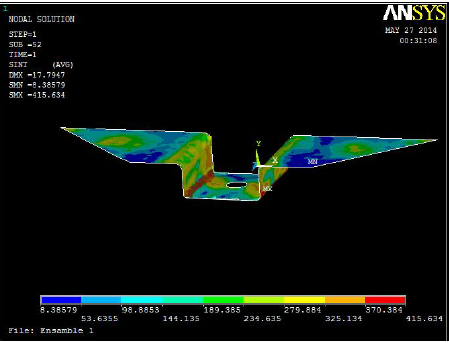
\includegraphics[width=0.7\textwidth]{src/ch1/olivera.png}
\captionof{figure}{Estado de esfuerzos para el análisis realizado por Olivera \cite{olivera2014}}
\label{fig:olivera}
\end{center}

Natalia García en \cite{garcia2009} realizó una simulación por elementos finitos del proceso de 
embutición de una chapa que sirve como pieza de soporte de la llanta de repuesto de un automóvil. 
Utilizó un enfoque dinámico explícito para la simulación. El análisis realizado consta 
de 4 etapas, realizadas progresivamente, para cada una de las cuales ejecutó varios análisis 
variando las propiedades del material utilizado, así como las velocidades de trabajo, con la 
finalidad de obtener una velocidad de embutición adecuada y la reducción del peso de la pieza.\\

Arwidson \cite{arwidson2005} realizó una comparación del comportamiento de cuatro materiales (aceros de
alta resistencia) en un proceso de estampado mediante una simulación por elementos finitos
utilizando dos software: PamStamp y LS-DYNA. Lo anterior buscando encontrar un modelo 
numérico y las condiciones de frontera adecuadas para el proceso, además de simular
el fenómeno de la recuperación elástica (springback) utilizando Abaqus, para determinar la
sobre-deformación a aplicar con el herramental. De acuerdo a los resultados, Arwidson estima
que las mayores deformaciones se sobrevaloran en alrededor de un 75 \% en las regiones sometidas 
a flexión crítica. Reporta también que la variación del coeficiente de fricción en el rango 
de 0 a 0.1 tiene una influencia casi nula en la simulación del proceso de estampado. \\

% \begin{center}
% 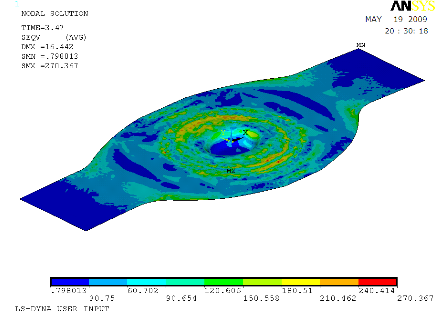
\includegraphics[width=0.6\textwidth]{src/ch1/garcia2009.png}
% \captionof{figure}{Estado de esfuerzos esquivalentes en pieza analizada por García \cite{garcia2009}}
% \label{fig:garcia2009}
% \end{center}

Lindberg \cite{lindberg2012} evaluó la implementación de un software de simulación por elemento finito 
(LS-DYNA) en el proceso de diseño de herramentales de la compañía Duroc Tooling, buscando
reducir los grandes costos derivados de errores en el proceso de diseño. Desarrolló un modelo
de elemento finito para un elemento estructural producido mediante un proceso de estampado, 
y evaluó los beneficios reportados por la simulación: tales como la identificación de grietas,
arrugas o cualquier tipo de debilitamiento en la chapa. Respecto a la parte económica hace
hincapié en el costo de una licencia de un software de este tipo, resultando redituable para 
cuando una compañía desarrolla más de una decena de herramentales anualmente, si por el
contrario desarrolla unas pocas herramientas, entonces resultaría mejor pagar a una empresa
externa por cada simulación.\\

Para la simulación numérica de procesos de formado de tubo mediante doblados sucesivos en UO, 
similares al proceso a desarrollar, se tienen algunos trabajos anteriores, en la mayoría de los 
casos son autores japoneses que desarrollaron códigos con un enfoque elasto-plástico.\\

Makinouchi \cite{makinouchi1989} desarrolló un código de computadora para analizar un proceso 
de deformación por doblado en UO bajo condiciones de deformación plana, obteniendo resultados 
satisfactorios y sobre todo un algoritmo muy eficiente.\\

Huang & Leu ~\cite{huang1995} desarrollaron un código de análisis elasto-plástico por elemento finito, 
basado en una formulación lagrangiana modificada, para simular proceso de doblado UO en placas metálicas, 
bajo condiciones de deformación plana. Para realizar el análisis del proceso completo, dividieron este 
en tres pasos de carga o configuraciones que se muestran en la figura ~\ref{fig:pasos_formado_01}, 
doblado en U, descarga y doblado final en O. Aplicaron además simetría debido a la disposicion de las 
herramientas y el blank a formar, simplificando aún más el análisis. Utilizaron un coeficiente 
de fricción de $\mu = 0.02$ y el espesor de la chapa fue de 6 mm. \\
% En la figura ~\ref{fig:shape_sequence} 
% se puede observar la secuencia del desarrollo de la geometría obtenida mediante el análisis realizado. \\

\begin{center}
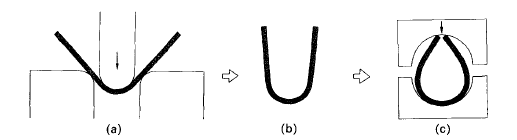
\includegraphics[width=0.75\textwidth]{src/ch1/uo-bending.png}
\captionof{figure}{Proceso de doblado UO, a) Doblado en U b) Descarga c) Doblado en O \cite{huang1995}}
 \label{fig:pasos_formado_01}
\end{center}

% \begin{center} \label{fig:shape_sequence}
% 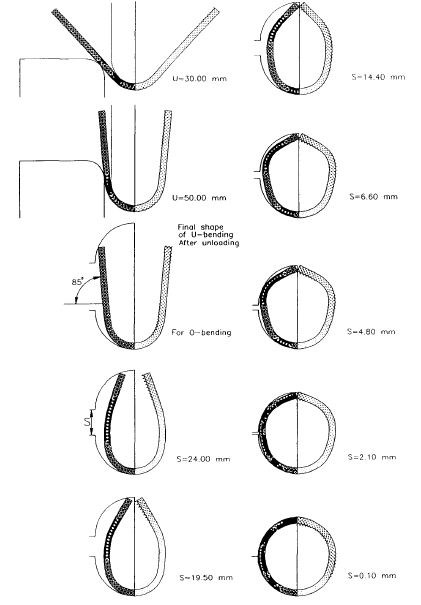
\includegraphics[scale=0.75]{src/ch1/shape_sequence.png}
% \captionof{figure}{Secuencia obtenida mediante el proceso de doblado UO. \cite{huang1995}}
% \end{center}

Chen y Huang ~\cite{chen2007} de manera similar a ~\cite{huang1995} simularon un proceso de doblado 
UO, con las mismas etapas: doblado en U, descarga y doblado en O. El espesor de lámina de la pieza 
de trabajo fue de 6 mm y un ancho de 10 mm. Utilizaron una ecuación exponencial para la relación 
esfuerzo-deformación. Los resultados obtenidos fueron la distribución 
de esfuerzos de von Mises y la forma geométrica resultante, medidas para ciertos intervalos 
de desplazamiento del punzon formador superior. \\

% \begin{center}
% 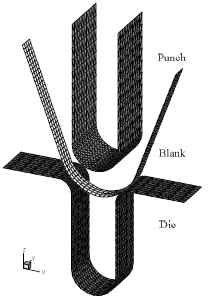
\includegraphics[scale=0.65]{src/ch1/u_bend.png}
% \captionof{figure}{Modelo de elementos finitos del doblado en U \cite{chen2007}}
% \label{fig:u_bend}
% \end{center}

% \begin{center}
% 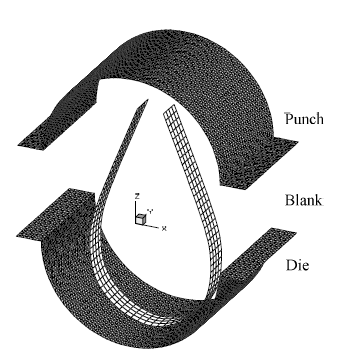
\includegraphics[scale=0.65]{src/ch1/o_bend.png}
% \captionof{figure}{Modelo de elementos finitos del doblado en O \cite{chen2007}}
% \label{fig:o_bend}
% \end{center}

Finalmente , García \cite{garcia2005} desarrolló un modelo de predicción del ángulo de recuperación y del 
radio de doblado final en procesos de doblado al aire, combinando técnicas de procesamiento digital 
de imágenes para el procesamiento y obtención de datos de la parte experimental, y el uso de redes neuronales 
para calcular el modelo de predicción a partir de la introducción de datos experimentales. En un enfoque 
similar, Rodríguez \cite{rodriguez2014} trabajó en el desarrollo de un modelo matemático que utilizó para 
optimizar parámetros de un doblado en U mediante las técnicas de nubes de partículas y algoritmo  genético, 
con la finalidad de obtener una relación que describiera de mejor manera el comportamiento de la recuperación 
elástica.
% Lo que debería contener este capítulo
% 
% Procesos de estampado
% Propiedades de materiales (Elasticidad / Plasticidad)
% Modelos constitutivos
% Método del elemento finito
% Teoría de contactos
% 
\chapter{Marco teórico}

\section{Procesos de formado}

El formado de metales incluye varios procesos de manufactura en los cuales se usa la deformación 
plástica para cambiar la forma de las piezas metálicas. La deformación es el resultado del uso de 
una herramienta que generalmente es un troquel para formar metales, mediante el cual se aplican 
esfuerzos que exceden la resistencia a la fluencia, induciendo una deformación plástica 
~\cite{groover2007}\\.

Normalmente, se aplica un esfuerzo de compresión para deformar plásticamente el metal, no obstante, 
algunos procesos de formado estiran, cortan o doblan el metal. Para que un metal sea adecuado 
como materia prima en un proceso de formado, este debe poseer ciertas propiedades mecánicas, 
tales como una baja resistencia a la fluencia y alta ductilidad, para facilitar la deformación 
plástica. Además, debe tenerse en cuenta el factor de la temperatura, mismo que determina 
la clasificación de trabajo en frío y caliente (referente a la temperatura de cristalización). 
También la velocidad de formación y el fenómeno de fricción entre la pieza metálica y el herramental 
son factores adicionales que afectan el desempeño del formado de metales.\\

\subsection{Tipos de formado}

Los procesos de formado se pueden clasificar en dos categoría generales, a saber: procesos de 
deformación volumétrica y procesos de trabajo de láminas metálicas.~\cite{groover2007}\\

Los \textbf{procesos de deformación volumétrica} se caracterizan por deformaciones significativas 
que derivan en grandes cambios de forma, y la relación entre el área superficial y el volumen 
de trabajo es relativamente pequeña. Algunos tipos de formado que entran dentro de esta 
clasificación son: rolado, forjado, extrusión y estirado.\\

Los \textbf{procesos de trabajo de láminas metálicas} son operaciones de formado o preformado 
de láminas, tiras y rollo de metal. La razón entre el área superficial y el volumen del material 
inicial es alta, por lo que esta relación es un medio útil para distinguir la deformación 
de los procesos descritos anteriormente. Estas operaciones se ejecutan siempre en frío y 
se utiliza un herramental compuesto en la mayoría de los casos de un conjunto de formadores, 
conocidos comúnmente como punzones y matrices en el ámbito industrial. Se pueden 
distinguir de manera general tres tipos de operaciones que entran en esta clasificación: 
doblado, estirado y corte.\\

En este caso centraremos el interés en esta última clasificación, puesto que el proceso 
de formado del tubo se realiza utilizando una combinación de corte-doblado.

\subsection{Herramentales (troqueles)}

Los herramentales utilizados en los procesos de formado (comúnmente llamados troqueles) son 
construidos teniendo en cuenta algunos aspectos elementales, a saber ~\cite{marin2009}:

\begin{enumerate}
\item Trabajo a realizar 
\item Características de la prensa
\item Material a troquelar
\item Número de piezas a producir
\end{enumerate}

\subsubsection{Tipos de troqueles}

A medida que aumentan los requerimientos del trabajo, la capacidad de las prensas, las exigencias 
de los materiales y la necesidad de producir más y mejor, también se conciben los diseños de 
troqueles con mayor complejidad y desarrollo. En ese sentido, los troqueles se pueden clasificar 
en simples, compuestos y progresivos.\\

\textbf{Simples}: estos troqueles permiten realizar solamente una operación por cada golpe o 
ciclo de la prensa, lo cual implica una bajo volumen de producción y productividad, y 
siendo normalmente necesario el uso de más de un herramental para terminar el producto.\\

\textbf{Compuestos}: permiten aprovechar la fuerza ejercida por la prensa realizando dos 
o más operaciones en cada golpe, agilizando el proceso y elevando en cierto punto 
la productividad.\\

\textbf{Progresivos}: son troqueles complejos y de gran desarrollo. Constan de una 
cantidad considerable de etapas, en cada uno de ellos se modifica la lámina con una secuencia 
establecida durante el diseño y acorde a los requerimientos del producto, de tal manera 
que al final se obtiene una o varias piezas terminadas. Naturalmente son altamente productivos, 
aunque su mantenimiento y operación es más compleja que en los casos anteriores.

\subsubsection{Componentes de un troquel}

Los componentes de un troquel varían dependiendo del tipo, pero típicamente hay elementos 
que se encuentran en casi todos los troqueles y que cumplen con funciones específicas 
en el proceso de formado.\\

\textbf{Base superior}. Contiene en su interior todas las placas y elementos que sostienen 
los punzones del troquel, está anclada a la prensa. Algunos elementos alojados en 
la parte superior son: placa porta-punzones, punzones, sufrideras, postes, pisadores, resortes, 
entre otros elementos adicionales.\\

\textbf{Base inferior}. Es el elemento sobre el cual van montados todos los componentes 
que hacen la parte de la matriz, y a su vez, está fuertemente sujeta en la bancada 
de la prensa durante la fase de trabajo. Algunos de los elementos contenidos en 
la base inferior son: placa  porta-matrices, guías, sufrideras, topes de avance, entre 
otros.\\

\textbf{Sufrideras}. La función básica de las placas superior e inferior de choque o sufrideras 
consiste en absorber sobre su superficie los sucesivos golpes de los elementos en el troquel. 
Estos impactos se producen cada vez que los punzones transforman la lámina con la matriz. Cuando 
el punzón impacta contra el material, la resistencia que opone este es transmitida a la 
superficie de las sufrideras sobre las que se apoyan las placas porta matriz y porta punzones. 
Estas placas están construidas en materiales ya templados y que conservan su tenacidad y cohesión, 
uno muy empleado es el acero SAE/AISI 1045.\\

\textbf{Porta punzones}. La finalidad de la placa porta punzones es la de alojar y fijar en 
su interior todos los punzones que lleve la matriz. Estos punzones pueden ser de cualquier 
tipo o tamaño pero han de tener una sola carcterística en común: deben estar firmemente 
sujetos y guiados en el interior de dicha placa impidiendo que puedan moverse o desprenderse.\\

\textbf{Porta matriz}. La placa porta matrices aloja y posiciona en su interior todos 
los elementos de pequeñas dimensiones que lleve la propia matriz, de esta manera dichos componentes 
quedarán ajustados en su interior.\\

\textbf{Placa pisadora}. Durante el movimiento descendente del troquel, la placa pisadora presiona 
la lámina dejándola inmovilizada antes de que los punzones lleguen a tocarla y mientras penetran 
el material y lo transforman. Una vez cortada la lámina, la función de la placa es mantener la 
pieza bien sujeta hasta que los punzones hayan salido de ella, de lo contrario, los punzones 
la arrastrarían hacia arriba sujeta a ellos, con el riesgo de fractura.\\

\textbf{Punzones}. Los punzones tienen por objeto realizar las máximas transformaciones en la lámina 
a fin de obtener piezas con una calidad acorde a las medidas requeridas, hay tanto tipos de estos 
como variantes del troquelado.\\

\textbf{Matrices}. Las matrices son los elementos complementarios a los punzones, tienen la forma 
negativa de estos.

\begin{center}
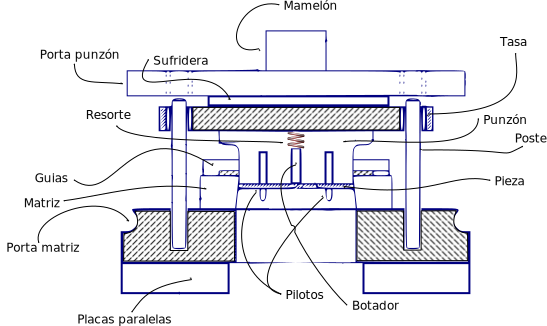
\includegraphics[scale=0.3]{src/ch2/componentes_troquel.png}
\captionof{figure}{Componentes de un troquel. \textit{Fuente:} ~\cite{wikiTroquel2008}}
\label{fig:componentes_troquel}
\end{center}

\section{Mecánica de sólidos}

\subsection{Relaciones constitutivas}

En el caso de un sólido tridimensional isotrópico la relación esfuerzo-deformación está dada por la Ley de Hooke, 
expresada en términos matemáticos como:

\begin{equation}\label{eq:ecdef}
\vec{\varepsilon} = 
\left\{\begin{matrix}
\varepsilon_{xx} \\ \varepsilon_{yy} \\ \varepsilon_{zz} \\ \varepsilon_{xy} \\ \varepsilon_{yz} \\ \varepsilon_{zx}
\end{matrix}\right\} = 
\left[ C \right] \vec{\sigma} + \vec{\varepsilon_0} = 
\left[ C \right]
\left\{\begin{matrix}
\sigma_{xx} \\ \sigma_{yy} \\ \sigma_{zz} \\ \sigma_{xy} \\ \sigma_{yz} \\ \sigma_{zx}
\end{matrix}\right\} + 
\left\{\begin{matrix}
\varepsilon_{xx}_0 \\ \varepsilon_{yy}_0 \\ \varepsilon_{zz}_0 \\ \varepsilon_{xy}_0 \\ \varepsilon_{yz}_0 \\ \varepsilon_{zx}_0
\end{matrix}\right\}
\end{equation}

Donde $[C]$ es la matriz de constantes elásticas definida por:

\begin{equation}
[C] = \frac{1}{E}
\left[\begin{matrix}
1 & -\nu & -\nu & 0 & 0 & 0 \\
-\nu & 1 & -\nu & 0 & 0 & 0 \\
-\nu & -\nu & 1 & 0 & 0 & 0 \\
0 & 0 & 0 & 2(1+\nu) & 0 & 0 \\
0 & 0 & 0 & 0 & 2(1+\nu) & 0 \\
0 & 0 & 0 & 0 & 0 & 2(1+\nu) \\
\end{matrix}\right]
\end{equation}

$\vec{\varepsilon_0}$ es el vector de esfuerzos iniciales, $E$ es el módulo de Young y $\nu$ el coeficiente de Poisson del 
material.\\

Algunas veces la expresión de esfuerzos en términos de deformaciones puede ser necesaria. Incluyendo las deformaciones 
térmicas, la ecuación \ref{eq:ecdef} puede ser invertida para obtener:

\begin{equation}
\vec{\sigma} = 
\left\{\begin{matrix}
\sigma_{xx} \\ \sigma_{yy} \\ \sigma_{zz} \\ \sigma_{xy} \\ \sigma_{yz} \\ \sigma_{zx}
\end{matrix}\right\} = 
\left[ D \right] (\vec{\varepsilon} - \vec{\varepsilon_0})= 
\left[ D \right] 
\left\{\begin{matrix}
\varepsilon_{xx} \\ \varepsilon_{yy} \\ \varepsilon_{zz} \\ \varepsilon_{xy} \\ \varepsilon_{yz} \\ \varepsilon_{zx}
\end{matrix}\right\} - 
\frac{E\alpha T}{1-2\nu}
\left\{\begin{matrix}
1 \\ 1 \\ 1 \\ 0 \\ 0 \\ 0
\end{matrix}\right\} 
\end{equation}

Donde la matriz $[D]$ está dada por:

\begin{equation}
[C] = \frac{E}{(1+\nu)(1-2\nu)}
\left[\begin{matrix}
1-\nu & \nu & \nu & 0 & 0 & 0 \\
\nu & 1-\nu & \nu & 0 & 0 & 0 \\
\nu & \nu & 1-\nu & 0 & 0 & 0 \\
0 & 0 & 0 & \frac{1-2\nu}{2} & 0 & 0 \\
0 & 0 & 0 & 0 & \frac{1-2\nu}{2} & 0 \\
0 & 0 & 0 & 0 & 0 & \frac{1-2\nu}{2} \\
\end{matrix}\right]
\end{equation}

En el caso de problemas bidimensionales, dos tipos de distribuciones de esfuerzos son posibles: esfuerzo plano 
y deformación plana.

\subsubsection{Esfuerzo plano}

La consideración de esfuerzo plano es aplicable para cuerpos en los cuales su dimensión en una dirección es muy 
pequeña comparada con las otras. En el caso de esfuerzo plano se asume que:

\begin{equation}
\sigma_{zz} = \sigma_{zx} = \sigma_{yz} = 0
\end{equation}

Donde $z$ representa la dirección perpendicular al plano de la placa mostrada en la figura \ref{fig:fg1}, 
y los componentes de esfuerzo no varían a través del espesor de la placa.

\begin{center}
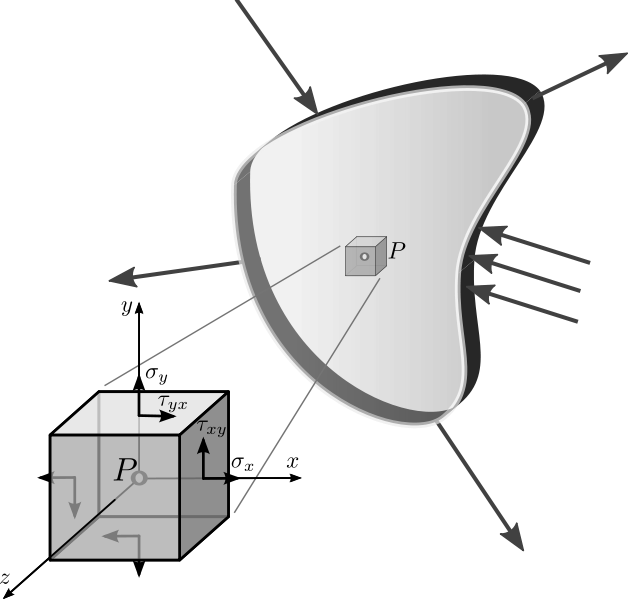
\includegraphics[scale=0.35]{src/ch2/plane_stress.png}
\captionof{figure}{Esfuerzo plano}
\label{fig:fg1}
\end{center}

Entonces, las relaciones esfuerzo deformación se reducen a:

\begin{equation}
\vec{\varepsilon} = [C] \vec{\sigma} + \vec{\varepsilon_0}
\end{equation}

donde:

\begin{equation}
\vec{\varepsilon} = 
\left\{\begin{matrix}
\varepsilon_{xx} \\ \varepsilon_{yy} \\ \varepsilon_{xy}
\end{matrix}\right\}
\end{equation}

\begin{equation}
\vec{\sigma} = 
\left\{\begin{matrix}
\sigma_{xx} \\ \sigma_{yy} \\ \sigma_{xy}
\end{matrix}\right\}
\end{equation}

\begin{equation}
[C] = \frac{1}{E}
\left[\begin{matrix}
1 & -\nu & 0 \\
-\nu & 1 & 0 \\
0 & 0 & 2(1+\nu) \\
\end{matrix}\right]
\end{equation}

\begin{equation}
\vec{\varepsilon_0} = 
\left\{\begin{matrix}
\varepsilon_{xx_0} \\ \varepsilon_{yy_0} \\ \varepsilon_{xy_0}
\end{matrix}\right\} =
\alpha T 
\left\{\begin{matrix}
1 \\ 1 \\ 0 \\
\end{matrix}\right\}
\end{equation}

En el caso de deformaciones térmicas,

\begin{equation}
\vec{\sigma} = [D] (\vec{\varepsilon} - \vec{\varepsilon_0}) = 
[D] \vec{\varepsilon} - 
\frac{E\alpha T}{1-\nu} 
\left\{\begin{matrix}
1 \\ 1 \\ 0 \\
\end{matrix}\right\}
\end{equation}

Con, 

\begin{equation}
[D] = \frac{E}{1-\nu^2}
\left[\begin{matrix}
1 & \nu & 0 \\
\nu & 1 & 0 \\
0 & 0 & \frac{1-\nu}{2} \\
\end{matrix}\right]
\end{equation}

En el caso de esfuerzo plano la componente de la deformación en el plano $z$, será diferente de cero, debido al 
efecto del coeficiente de Poisson, estando dada  por la expresión:

\begin{equation}
\varepsilon_{zz} = -\frac{\nu}{E} (\sigma_{xx} + \sigma_{yy}) + \alpha T = 
\frac{-\nu}{1-\nu} (\varepsilon_{xx} + \varepsilon_{yy}) +  
\frac{1+\nu}{1-\nu} \alpha T
\end{equation}

Mientras que, 

\begin{equation}
\varepsilon_{yz} = \varepsilon_{zx} = 0
\end{equation}


\subsubsection{Deformación plana}

La consideración de deformación plana es aplicable para sólidos largos y cuya geometría y cargas no varían de 
manera significativa en la dirección longitudinal.\\

En este caso las ecuaciones de esfuerzo-deformación tridimensional se reducen a:

\begin{equation}
\vec{\varepsilon} = [C] \vec{\sigma} + \vec{\varepsilon_0}
\end{equation}

donde:

\begin{equation}
\vec{\varepsilon} = 
\left\{\begin{matrix}
\varepsilon_{xx} \\ \varepsilon_{yy} \\ \varepsilon_{xy}
\end{matrix}\right\}
\end{equation}

\begin{equation}
\vec{\sigma} = 
\left\{\begin{matrix}
\sigma_{xx} \\ \sigma_{yy} \\ \sigma_{xy}
\end{matrix}\right\}
\end{equation}

\begin{equation}
[C] = \frac{1+\nu}{E}
\left[\begin{matrix}
1-\nu & -\nu & 0 \\
-\nu & 1-\nu & 0 \\
0 & 0 & 2 \\
\end{matrix}\right]
\end{equation}

\begin{equation}
\vec{\varepsilon_0} = 
\left\{\begin{matrix}
\varepsilon_{xx_0} \\ \varepsilon_{yy_0} \\ \varepsilon_{xy_0}
\end{matrix}\right\} =
(1+\nu) \alpha T 
\left\{\begin{matrix}
1 \\ 1 \\ 0 \\
\end{matrix}\right\}
\end{equation}

En el caso de deformaciones térmicas,

\begin{equation}
\vec{\sigma} = [D] (\vec{\varepsilon} - \vec{\varepsilon_0}) = 
[D] \vec{\varepsilon} - 
\frac{E\alpha T}{1-2\nu} 
\left\{\begin{matrix}
1 \\ 1 \\ 0 \\
\end{matrix}\right\}
\end{equation}

Con, 

\begin{equation}
[D] = \frac{E}{(1+\nu)(1-2\nu)}
\left[\begin{matrix}
1-\nu & \nu & 0 \\
\nu & 1-\nu & 0 \\
0 & 0 & \frac{1-2\nu}{2} \\
\end{matrix}\right]
\end{equation}

\begin{center}
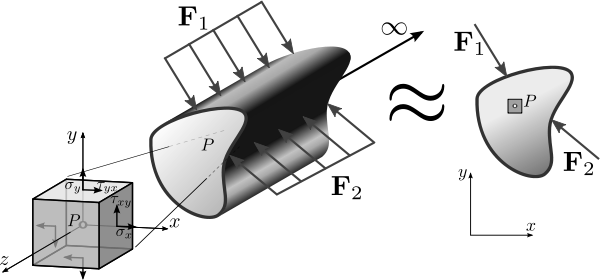
\includegraphics[scale=0.55]{src/ch2/plane_strain.png}
\captionof{figure}{Deformación plana}
\label{fig:fg2}
\end{center}

El componente de esfuerzo en la dirección $z$ no será nulo debido a los efectos del coeficiente de Poisson, y está 
dado por:

\begin{equation}
\sigma_{zz} = \nu(\sigma_{xx}+\sigma_{yy}) - E \alpha T
\end{equation}

y, 

\begin{equation}
\sigma_{yz} = \sigma_{zx} = 0
\end{equation}

\subsection{Relaciones deformación-desplazamiento}

La forma deformada de un cuerpo elástico bajo una determinada configuración de cargas y distribución de temperaturas 
pueden ser descritas completamente por tres componentes de desplazamiento $u, v$ y $w$ paralelas a las direcciones 
$x, y$ y $z$ respectivamente. En general, cada una de estas componentes $u,v$ y $w$ es una función de las 
coordenadas $x,y$ y $z$. Las deformaciones inducidas en el sólido pueden ser expresadas en términos de los 
desplazamientos $u,v$ y $w$.\\

Si los desplazamientos se consideran muy pequeños, la deformaciones pueden ser expresadas como:

\begin{subequations}
\begin{eqnarray}
\varepsilon_{xx} = \frac{du}{dx} \\
\varepsilon_{yy} = \frac{dv}{dy} \\
\varepsilon_{zz} = \frac{dw}{dz} \\
\varepsilon_{xy} = \frac{du}{dy} + \frac{dv}{dx} \\
\varepsilon_{yz} = \frac{dw}{dy} + \frac{dv}{dz} \\
\varepsilon_{zx} = \frac{du}{dz} + \frac{dw}{dx} \\
\end{eqnarray}
\end{subequations}

\subsection{Plasticidad}

La teoría de plasticidad estudia la fluencia de materiales bajo estados de esfuerzos complejos. Permite 
conocer si un material cederá bajo ciertas condiciones de esfuerzo y determinar el cambio en la forma o 
geometría en caso de que la fluencia ocurra. También permite usar datos de ensayos de tensión para predecir 
el endurecimiento por carga durante la deformación bajo complejos estados de esfuerzo. Estas relaciones 
son parte fundamental de los códigos de computadora utilizados para predecir la capacidad de una estructura 
para absorber impactos, así como en procesos de formado o estampado que involucran la deformación plástica de 
placas metálicas.

\subsubsection{Criterio de fluencia}

Un criterio de fluencia es una expresión matemática propuesta del estado de esfuerzo que causará la fluencia. La forma más general es:

\begin{equation}
f(\sigma_x,\sigma_y, \sigma_z, \tau_{yz}, \tau_{zx}, \tau_{xy} ) = C 
\end{equation}

Para materiales isotrópicos esto puede ser expresado en términos de los esfuerzos principales como:

\begin{equation}
f(\sigma_1,\sigma_2,\sigma_3 )=C
\end{equation}

Para la mayoría de los metales dúctiles isotrópicos comúnmente se hacen las siguientes consideraciones:

\begin{itemize}
\item El esfuerzo de fluencia en tensión y compresión es el mismo.
\item El volumen permanece constante durante la deformación plástica
\item La magnitud del esfuerzo normal promedio, no afecta la fluencia.
\end{itemize}

\begin{equation}
\sigma_m=\frac{\sigma_1+\sigma_2+\sigma_3}{3}
\end{equation}

La consideración que la fluencia es independiente de $\sigma_m$ es razonable porque la deformación usualmente ocurre por deslizamiento o mecanismos de corte. Por lo tanto los criterios de fluencia para materiales isotrópicos tienen la forma:

\begin{equation}
f[(\sigma_2-\sigma_3 ),(\sigma_3-\sigma_1 ),(\sigma_1-\sigma_2 )] = C
\end{equation}

\subsubsection{Criterio de Tresca}

El criterio más simple es uno de los primero propuestos por Tresca. Afirma que la cedencia ocurrirá cuando el máximo 
esfuerzo cortante alcance un valor crítico. El máximo esfuerzo cortante viene dado por:

\begin{equation}
\tau_{max} = \frac{\sigma_{max}-\sigma_{min}}{2}
\end{equation}

entonces, el criterio de Tresca puede expresarse como:

\begin{equation}
\sigma_{max} - \sigma_{min} = C
\end{equation}

Si se mantiene la convención de que $ \sigma_1 \me \sigma_2 \me \sigma_3 $, puede reescribirse lo anterior como:

\begin{equation}\label{eq:ec1}
\sigma_1 - \sigma_3 = C
\end{equation}

La constante C puede ser encontrada mediante un ensayo de tensión uniaxial. En un ensayo de tensión, 
$\sigma_2 = \sigma_3 = 0$ y la cedencia $\sigma_1 = Y$, donde $Y$ es el esfuerzo de fluencia. Sustituyendo 
en $C=Y$ en la ecuación \ref{eq:ec1}. Por lo tanto el criterio de Tresca puede ser expresado como:

\begin{equation}\label{eq:ec2}
\sigma_1 - \sigma_3 = Y
\end{equation}

Para cortante puro, $ \sigma_1 = -\sigma_3 = k$, donde $k$ es esfuerzo de fluencia por cortante. Sustituyendo 
$ k = Y/2 $ en la ecuación \ref{eq:ec2}, entonces:

\begin{equation}
\sigma_1 - \sigma_3 = 2k = C
\end{equation}

\subsubsection{Criterio de Von Mises}

El efecto del esfuerzo principal medio puede ser incluido asumiendo que la fluencia depende de la raíz cuadrada 
del promedio de los diámetros de los tres círculos de Mohr. Este es el criterio de Von Mises, el cual puede ser 
expresado como:

\begin{equation} \label{eq:ec3}
\left\{ [(\sigma_2-\sigma_3)^2 + (\sigma_3-\sigma_1 )^2 + (\sigma_1-\sigma_2 )^2]/3 \right\}^{1/2} = C
\end{equation}

Como cada término está elevado al cuadrado, la convención $\sigma_1 \me \sigma_2 \me \sigma_3$ no es necesaria. 
La constante del material, $C$, puede ser evaluada mediante un ensayo de tensión uniaxial. En la fluencia, 
$\sigma_1 = Y$ y $\sigma_2 = \sigma_3 = 0$. Sustituyendo, $[0^2 + (-Y)^2 + Y^2]/3 = C^2$, o 
$C = (2/3)^{1/3} Y $, entonces, la ecuación usualmente se escribe como:

\begin{equation}\label{eq:ec4}
(\sigma_2-\sigma_3)^2 + (\sigma_3-\sigma_1 )^2 + (\sigma_1-\sigma_2 )^2 = 2Y^2
\end{equation}

Para cortante puro, $\sigma_1 = -\sigma_3 = k$ y $\sigma_2=0$. Sustituyendo en la ecuación \ref{eq:ec4}, 
$ (-k)^2 + [ (-k)-k ]^2 + k^2 = 2Y^2 $, entonces:

\begin{equation}\label{eq:ec5}
k = Y/\sqrt{3}
\end{equation}

La ecuación \ref{eq:ec5} puede ser simplificada si uno de los esfuerzos principales es cero (condición de esfuerzo plano). 
Sustituyendo $\sigma_3 = 0$, $\sigma_1^2 + \sigma_2^2 - \sigma_1 \sigma_2 = Y^2$, el cual es una elipse. Con la 
consiguiente sustitución de $\alpha = \sigma_2/\sigma_1$,

\begin{equation}
\sigma_1 = Y/(1-\alpha+\alpha^2)^{1/2}
\end{equation}


% \subsection{Ecuaciones de equilibrio}

% \subsubsection{Equilibrio externo}

% Si un sólido está en equilibrio bajo ciertas condiciones de carga, las fuerzas reactivas y momentos desarrollados en 
% los puntos de soporte deben balancear las fuerzas y momentos externos aplicados. Haciendo referencia a la figura 
% \ref{fig:externalforces}, sean $\phi_x, \phi_y, \phi_z$ las fuerzas de cuerpo, $\Phi_x, \Phi_y, \Phi_z$ las 
% fuerzas de superficie, $P_x, P_y, P_z$ las fuerzas concentradas externas, y $Q_x, Q_y, Q_z$ los momentos externos 
% aplicados. Entonces, las ecuaciones de equilibrio externo pueden establecerse como:

% \begin{eqnarray}
% \int_S \Phi_x ds + \int_V \phi_x dV + \sum P_x = 0 \nonumber \\
% \int_S \Phi_y ds + \int_V \phi_y dV + \sum P_y = 0 \\
% \int_S \Phi_z ds + \int_V \phi_z dV + \sum P_z = 0 \nonumber
% \end{eqnarray}

% \begin{center}
% 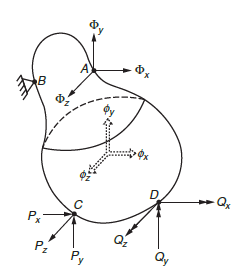
\includegraphics[scale]{src/ch2/equillibrium_force.png}
% \captionof{figure}{Fuerzas de equilibrio externo}
% \label{fig:externalforces}
% \end{center}

% Para el equilibrio de momentos:

% \begin{eqnarray}
% \int_S (\Phi_zy - \Phi_{y}z) ds + \int_V (\phi_zy - \phi_{y}z) dV + \sum Q_x = 0 \nonumber \\
% \int_S (\Phi_x z - \Phi_z x) ds + \int_V (\phi_x z - \phi_z x) dV + \sum Q_y = 0 \\
% \int_S (\Phi_{y}x - \Phi_x y) ds + \int_V (\phi_{y}x - \phi_x y) dV + \sum Q_z = 0 \nonumber
% \end{eqnarray}

% Donde $S$ es la superficie y $V$ el volumen del cuerpo sólido.


% \subsubsection{Equilibrio interno}

% Debido a las aplicación de cargas, se desarrollan esfuerzos dentro del sólido. Si consideramos 
% un elemento de material dentro del sólido, este debería estar en equilibrio debido a esos 
% esfuerzos internos desarrollados.\\

% Teoricamente, el estado de esfuerzos en cualquier punto de un cuerpo cargado está completamente definido 
% en términos de nueve componentes de esfuerzo: $\sigma_{xx}, \sigma_{yy}, \sigma_{zz}, \sigma_{xy}, \sigma_{yx}, 
% \sigma_{yz}, \sigma_{zy}, \sigma_{zx}, \sigma_{xz} $, donde los primeros tres son las componentes normales y los restantes 
% son esfuerzos cortantes. Las ecuaciones de equilibrio interno relativas a los nueve componentes de esfuerzo pueden ser 
% obtenidas considerando el equilibrio de momentos y fuerzas actuando en el volumen elemental mostrado en 
% la figura \ref{fig:internalforces}. El equilibrio de momentos alrededor de los ejes $x,y,z$, asumiendo que no existen 
% momentos en el sólido, derivan en las siguientes relaciones:

% \begin{equation}
% \sigma_{yx} = \sigma_{xy}, \,\,\,\, \sigma_{zy} = \sigma_{yz}, \,\,\,\, \sigma_{xz} = \sigma_{zx}
% \end{equation}

% \begin{center}
% 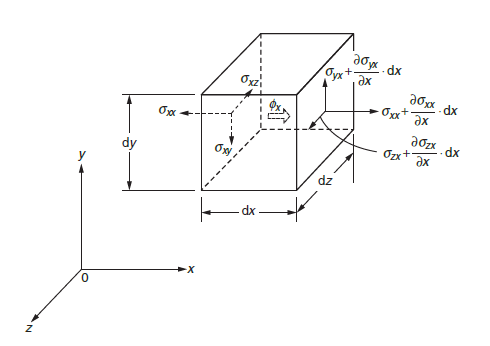
\includegraphics[scale]{src/ch2/internal_force.png}
% \captionof{figure}{Fuerzas de equilibrio interno}
% \label{fig:internalforces}
% \end{center}

% Estas ecuaciones muestran que el estado de esfuerzos en cualquier punto puede ser completamente definido por 
% los seis componentes $\sigma_{xx}, \sigma_{yy}, \sigma_{zz}, \sigma_{xy}, \sigma_{yz}, \sigma_{zx} $. 
% El equilibrio de fuerzas en las direcciones $x,y,z$ proporcionan las siguientes ecuaciones diferenciales de 
% equilibrio:

% \begin{eqnarray}
% \frac{\partial \sigma_{xx}}{\partial x} + \frac{\partial \sigma_{xy}}{\partial y} + 
% \frac{\partial \sigma_{zx}}{\partial z} + \phi_{x} = 0 \nonumber \\
% \frac{\partial \sigma_{xy}}{\partial x} + \frac{\partial \sigma_{yy}}{\partial y} + 
% \frac{\partial \sigma_{yz}}{\partial z} + \phi_{y} = 0 \\
% \frac{\partial \sigma_{zx}}{\partial x} + \frac{\partial \sigma_{yz}}{\partial y} + 
% \frac{\partial \sigma_{zz}}{\partial z} + \phi_{z} = 0 \nonumber
% \end{eqnarray}

% donde $\phi_x, \phi_y$ y $\phi_z$, son las fuerzas de cuerpo por unidad de volumen actuando a lo largo 
% de las direcciones $x,y$ y $z$, respectivamente.\\

% Para un problema bidimensional, existen solamente tres componentes de esfuerzo independientes, 
% $(\sigma_{xx},\sigma_{yy},\sigma_{xy})$ y las ecuaciones de equilibrio se reducen a:

% \begin{eqnarray}
% \frac{\partial \sigma_{xx}}{\partial x} + \frac{\partial \sigma_{xy}}{\partial y} + \phi_x = 0 \nonumber \\
% \frac{\partial \sigma_{xy}}{\partial x} + \frac{\partial \sigma_{yy}}{\partial y} + \phi_y = 0 
% \end{eqnarray}

% En problemas unidimensionales, sólo estará presente un componente de esfuerzo: $\sigma_{xx}$. Entonces, 
% las ecuaciones de equilibrio se reducen a:

% \begin{equation}
% \frac{\partial \sigma_{xx}}{\partial x} + \phi_x = 0
% \end{equation}

\section{El método de los elementos finitos}

\subsection{Generalidades del método}

En el método de elementos finitos se considera un cuerpo continuo o sólido, como un ensamble de pequeñas subdivisiones llamadas elementos finitos. Estos elementos están interconectados a través de nodos comunes. Debido a que la variación real de las variables de campo (desplazamientos, esfuerzos, temperaturas, etc.) se desconoce en el continuo, se asume que la variación de estas en el modelo de elemento finito puede ser aproximada por una simple función. Estas funciones de aproximación, también llamadas modelos de interpolación, son definidas en términos de los valores nodales de las variables de campo.\\

En general, el método de los elementos finitos, consiste en formular un sistema de ecuaciones (ecuaciones de equilibrio) para el sistema continuo que ha sido discretizado, donde las incógnitas suelen ser los valores nodales de las variables de campo. Luego, se resuelve este sistema de ecuaciones, con las consideraciones correspondientes a las condiciones de frontera o valores iniciales que simplifiquen el modelo original. La siguiente ecuación muestra, en notación matricial, el sistema de ecuaciones resuelto en una formulación de elemento finito.

\begin{equation}
K\,\bm{u} = \bm{P}
\end{equation}

Donde $K$ es la matriz global de rigidez, $\bm{u}$ es el vector de desplazamientos nodales y $\bm{P}$ el 
vector de fuerzas nodales en el sistema.\\

Para problemas lineales, el vector $\bm{u}$ puede ser resuelto de manera sencilla, mediante 
procedimientos básicos del álgebra lineal. Sin embargo, para problemas no lineales, la solución 
tiene que ser obtenida mediante una secuencia de pasos, en el cual cada uno de estos implica la 
modificación de la matriz de rigidez $K$ y/o el vector global de carga $\bm{P}$.\\

En problemas de análisis dinámico, desplazamientos, velocidades, deformaciones, esfuerzos y cargas 
son dependientes del tiempo. Por ello deben incluirse algunos otros términos, por lo que la ecuación 
a resolver viene dada por la expresión siguiente:

\begin{equation}
M\ddot{\bm{u}} + C\dot{\bm{u}} ̇+ K\bm{u} = \bf{P}
\end{equation}

Donde $C\,\dot{u}$ representa las fuerzas viscosas, mismas que deben incluirse cuando el 
sistema esté amortiguado artificialmente.

% Primeramente, como en el caso estático, se debe idealizar el sólido en módelo de elementos finitos. 
% Luego, se asume que los desplazamientos del elemento $e$ se pueden definir como:

% \begin{equation}\label{eq:dynec1}
% \vec{U}(x,y,z,t) = 
% \left\{ \begin{matrix}
% u(x,y,z,t) \\ v(x,y,z,t) \\ w(x,y,z,t) \\
% \end{matrix} \right\} = 
% [N(x,y,z)] \vec{Q}^{(e)}(t)
% \end{equation}

% Donde $\vec{U}$ es el vector de desplazamientos, $[N]$ es la matriz de funciones de forma, y $\vec{Q}_{(e)}$ 
% es el vector de desplazamientos nodales que se considera como una función del tiempo.\\

% \begin{equation}
% [M] \ddot{\vec{Q}} + [K] \vec{Q} = \vec{P}
% \end{equation}

% Donde \ddot{\vec{Q}} es el vector de las aceleraciones nodales en el sistema global. Si se ignora 
% las ecuación de movimiento puede ser escrita como:


\subsection{Solución implícita vs explícita}

Existen, de manera general, dos tipos de métodos para resolver ecuaciones diferenciales  en problemas dependientes del tiempo: integración implícita e integración explícita. El método implícito de integración en el tiempo puede ser expresado como:
~\cite{nielsen1997}

\begin{equation}
u_{n+1}=f(\dot{u}_{n+1},\ddot{u}_{n+1},u_n,\dot{u}_n,…)
\end{equation}

y el método explícito como:

\begin{equation}
u_{n+1}=f(u_n,\dot{u}_n,\ddot{u}_n,u_{n-1},\dot{u}_{n-1},…)
\end{equation}

El método implícito requiere conocer las derivadas temporales en el paso n+1, las cuales son desconocidas, mientras el método explícito está basado en los valores conocidos en el paso n. Si el problema es no lineal, el método implícito necesita un procedimiento iterativo para determinar los nuevos desplazamientos. Con el método explícito los nuevos desplazamientos se determinan directamente de los valores conocidos en pasos previos, evitando el uso de iteraciones adicionales.\\

La simulación de estampados se caracteriza por las diversas no linealidades presentes, debidas al material, y a los contactos entre los diversos cuerpos analizados. Sin embargo, usando la integración explícita estas no linealidades pueden ser tratadas sin mayores problemas. Por ello, en la mayoría de las simulaciones de estampados suelen ser conveniente el uso de algoritmos de integración explícita.

\subsection{Contactos}



% \section{Teoría de contactos}

% \subsection{Introducción}

% Considere el movimiento dependiente del tiempo de dos cuerpos ocupando las regiones $B^1$ y $B^2$ 
% en su configuración deformada en el tiempo cero. Asuma que la intersección

% $$
% B^1 \cap B^2 = \emptyset
% $$

% es satisfecha. Sean $\partial B^1$ y $\partial B^1$ quienes denotan las fronteras de $B^1$ y $B^2$ 
% respectivamente. En un tiempo posterior, estos cuerpos ocupan las regiones $b^1$ y $b^2$ delimitadas 
% por $\partial b^1$ y $\partial b^2$ como se muestra en la figura \ref{fig:refanddef}. Debido a que la 
% configuración deformada no puede penetrar:

% $$
% \left( b^1 - \partial b^1 \right) \cap b^2 = \emptyset
% $$

% Mientras $\left( \partial b^1 \cap \partial b^2 \right) = \emptyset$, las ecuaciones de movimiento 
% permanecen desacopladas. En las anteriores y siguientes ecuaciones, el superíndice derecho $\alpha$ 
% $(=1,2)$ denota el cuerpo al cual la cantidad hace referencia.

% \begin{center}
% 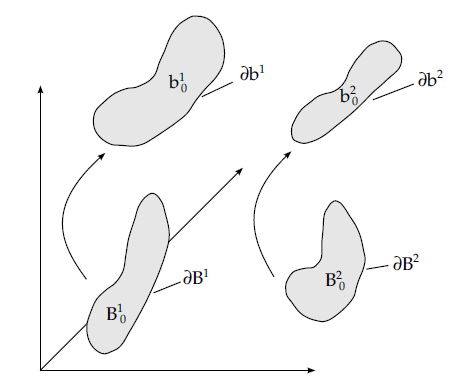
\includegraphics[scale=0.6]{src/ch2/ref_and_def.png}
% \captionof{figure}{Configuración de referencia y deformada}
% \label{fig:refanddef}
% \end{center}

% Antes de dar una descripción detallada de la teoría de contactos, algunos cuestiones adicionales 
% referentes a la terminología deben ser agregadas. Las superficies $\partial b^1$ y $\partial b^2$ 
% de los cuerpos discretizados $b^1$ y $b^2$ vienen a ser las superficies \textit{maestra} 
% y \textit{esclava}, respectivamente. La selección de las superficies maestra y esclava es 
% arbitraria cuando el tratamiento simétrico de penalización es utilizado. De lo contrario, 
% la superficie de malla más \textit{burda} debe ser elegida como maestra a menos que 
% exista una gran diferencia en las densidades de masa, en cuyo caso se recomienda definir 
% como superficie maestra al del material con mayor densidad de masa. Los puntos nodales 
% que definen $\partial b^1$ son llamados nodos maestros y los nodos que definen $\partial b^2$ 
% son llamados nodos esclavos. Cuando $\left( \partial b^1 \cap \partial b^2 \right) \neq \emptyset$, 
% las restricciones son impuestas para prevenir la penetración. Los superíndices derechos se 
% utilizan cuando una variable se refiere tanto a la superficie maestra $\partial b^1$ o 
% a la sueperficie esclava $\partial b^2$, consecuentemente estos superíndices se descartan 
% en el desarrollo siguiente.

% \subsection{\textit{Slave search}}

% Esta búsqueda encuentra para cada nodo esclavo su punto más cercano en la superficie maestra. 
% Las líneas dibujadas de un nodo esclavo a sus puntos más cercanos serán perpendiculares a la 
% superficie maestra, a menos que el punto se encuentre en la intersección de dos segmentos 
% maestros, donde un segmento está definido a ser un elemento de superficie de 3 o 4 nodos.\\

% Considere un nodo esclavo, $n_s$, deslizándose en una superficie maestra suave a tramos y 
% asuma que una búsqueda de la superficie maestra ha encontrado el nodo maestro, $m_s$, 
% situado cerca de $n_s$. La figura \ref{fig:slave_search} representa una porción 
% de una superficie maestra con nodos referenciados como $m_s$ y $n_s$. Si $m_s$ 
% y $n_s$ no coinciden, para $n_s$ por lo general se puede demostrar que se encuentra 
% en un segmento $s_1$  mediante el siguiente test:

% \begin{equation}
% (\mathbf{c_i} x \mathbf{s}) \cdot (\mathbf{c_i} x \mathbf{c_{i+1}}) > 0
% \end{equation}

% \begin{equation}
% (\mathbf{c_i} x \mathbf{s}) \cdot (\mathbf{s} x \mathbf{c_{i+1}}) > 0
% \end{equation}

% donde el vector $\mathbf{c_i}$ y $\mathbf{c_{i+1}}$

% \begin{center}
% 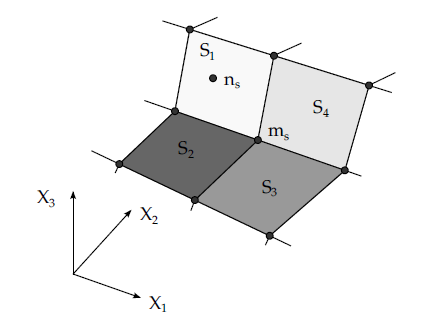
\includegraphics[scale=0.6]{src/ch2/slave_search.png}
% \captionof{figure}{Slave search}
% \label{fig:slave_search}
% \end{center}


% \subsection{Algoritmo de contacto superficie-superficie}

% Este implica un enfoque simétrico de dos pasos con un parámetro 
% de partición, $\beta$, que se establece entre la unidad positiva y negativa, donde $\beta=1$ 
% y $\beta=-1$ corresponden a tratamiento de una forma con la superficie \textit{maestra} 
% acumulando masa y fuerzas de la superficie \textit{esclava} (para $\beta = 1$) y viceversa 
% (para $\beta = -1$). ~\cite{lsdyna-manual} \\ 

% En este enfoque de restricción las aceleraciones, velocidades y desplazamientos se actualizan 
% primero a una configuración de prueba sin tener en cuenta las interacciones. Después de la 
% actualización, una fuerza de penetración es calculada para el nodo esclavo como una función 
% de la distancia de penetración $\Delta L$:

% $$
% \mathbf{\f_p} = \frac{m_s \Delta L}{\Delta t^2}\mathbf{n},
% $$

% Donde $\mathbf{n}$ es el vector normal a la superficie maestra.\\

% Se desea que la respuesta de la componente normal del vector de aceleración del nodo esclavo, 
% $\mathbf{a_s}$, de un nodo esclavo residiendo en un segmento maestro $k$ sea consistente con 
% el movimiento del segmento maestro en su porción de contacto $(s_c,t_c)$, por ejemplo:

% $$
% a_s = \phi_1 (s_c,t_c) a_{nk}^1 + \phi_2 (s_c,t_c) a_{nk}^2 + \phi_3 (s_c,t_c) a_{nk}^3 + \phi_4 (s_c,t_c) a_{nk}^4
% $$

% Para cada nodo esclavo en contacto y penetrando a través de la superficie maestra en 
% su configuración de prueba, su masa nodal y fuerza de penetración dadas por la ecuación 
% [REVISAR (Poner aquí referencia)] es acumulada a una masa y vector de fuerza global de 
% la superficie maestra.

% $$
% \left(
% m_k + \sum_s m_{ks}
% \right)
% \mathbf{a_{nk}}
% =
% \sum_s \mathbf{f_{ks}}
% $$

% donde:

% $$
% m_{ks} = \phi_k m_s
% $$

% $$
% \mathbf{f_{ks}} = \phi{k} \mathbf{f_s}
% $$

% Después de resolver la ecuación [REVISAR] para el vector de aceleración, $\mathbf{a_{nk}}$, podemos 
% obtener la corrección de aceleración para el nodo esclavo como:

% $$
% \mathbf{a_{ns}} = \mathbf{a_s} - \frac{f_p}{m_s}
% $$

% El proceso anterior es repetido después de invertir las definiciones de \textit{maestro-esclavo}. 
% En el paso final la corrección final promediada al vector de aceleración es encontrada:

% $$
% \mathbf{a_n^{final}} = \frac{1}{2} (1-\beta) \mathbf{a_n^{1st pass}} + 
% \frac{1}{2} (1-\beta) \mathbf{a_n^{2nd pass}} 
% $$

% Y se usa para calcular la aceleración final en el tiempo $n+1$

% $$
% \mathbf{a}^{n+1} = \mathbf{a}^{prueba} + \mathbf{a}_n^{final}
% $$

% La fricción resiste la velocidad tangencial relativa del nodo esclavo con respecto a 
% la superficie maestra. Esta velocidad relativa se expresa como:

% $$
% \mathbf{v_r} = \mathbf{v_s} - 
% \left(
% \phi_1 \mathbf{v}_k^1 + \phi_2 \mathbf{v}_k^2 + \phi_3 \mathbf{v}_k^3 + \phi_4 \mathbf{v}_k^4
% \right)
% $$

% la componente normal de la velocidad al segmento maestro:

% $$
% \mathbf{v_t} = \mathbf{v_r} - (\mathbf{n} \cdot \mathbf{v_r}) \mathbf{n}
% $$

% Una fuerza tangencial de prueba es calculada que cancelará la velocidad tangencial:

% $$
% \mathbf{f^{\ast}} = \frac{m_s v_t}{\Delta t}
% $$

% Donde $v_t$ es la magnitud del vector de velocidad tangencial.

% $$
% v_t = \sqrt{\mathbf{v}_t \cdot \mathbf{v}_t}
% $$

% La magnitud de la fuerza tangencial es limitada por la magnitud del producto de la constante de fricción 
% de Coulomb con la fuerza normal definido como:

% $$
% f_n = m_s \mathbf{a}_{ns} \cdot \mathbf{n}
% $$

% La fuerza limitada es, por lo tanto:

% $$
% F_y = m |\mathbf{f}_n|
% $$

% y 

% $$
% \mathbf{f}^{n+1} = \mathbf{f^{\ast}} \,\,\, if \,\,\, |\mathbf{f^{\ast}}| = F_y
% $$

% $$
% \mathbf{f}^{n+1} = \frac{F_y \mathbf{f^{\ast}}}{|\mathbf{f^{\ast}}|} \,\,\, if \,\,\, |\mathbf{f^{\ast}}| > F_y
% $$

% Por lo tanto, usando las ecuaciones anteriores la modificiación a la componente de  aceleración tangencial 
% del nodo esclavo está dado por:

% $$
% \mathbf{a_t} = \min\left( \mu \mathbf{a_{nt}} \cdot \mathbf{n} , \frac{|\mathbf{v_s}|}{\Delta t} \right)
% $$

% el cual debe actuar en la dirección del vector tangencial definido como:

% $$
% \mathbf{n_t} = \frac{\mathbf{v_t}}{v_t}
% $$

% Las correcciones a las componentes de aceleración del nodo esclavo y maestro son: 

% $$
% a_{ts} = a_{t} \mathbf{n_t}
% $$

% $$
% \mathbf{a_{tk}} = - \phi_k \frac{a_s m_s}{m_k} \mathbf{n_t}
% $$

% El proceso anterior se repite después de invertir la definición de esclavo y maestro. En el 
% paso final la corrección final promediada al vector de aceleración está dada por:

% $$
% \mathbf{a}_t^{final} = \frac{1}{2} \left( 1-\beta \right) \mathbf{a}_t^{1st pass}  + 
% \frac{1}{2} \left( 1 + \beta \right) \mathbf{a}_t^{2nd pass} 
% $$

% y es usado para calcular la aceleración final en el tiempo $n+1$: 

% $$
% \mathbf{a}^{n+1} = \mathbf{a}^{prueba}  +  \mathbf{a}_n^{final} + \mathbf{a}_t^{final}
% $$

% Una desventaja significativa del método de restricción respecto al método de penalización 
% aparece si un nodo de interfaz está sujeto a una restricción adicional como puntos de 
% soldadura, ecuaciones de restricción y cuerpos rígidos. Los cuerpos rígidos pueden 
% ser usados con estos algoritmos de contacto si sus movimientos están prescritos como 
% en el caso de los procesos de estampado. Para la mayoría de los casos que involucran 
% cuerpos rígidos, las ecuaciones anteriores no son directamente aplicables ya que las 
% masas nodales locales de los nodos de cuerpos rígidos son usualmente insignificantes. 
% Someter los dos lados de una superficie \textit{shell} a este algoritmo de contacto 
% también dará lugar a resultados erróneos, ya que un nodo de interfaz no puede 
% ser restringido a moverse simultáneamente en dos superficies mutuamente independientes.\\

% La mayor ventaja del algoritmo de restricción es que los nodos de interfaz permanecen 
% muy cerca de las superficies con las cuales están en contacto. Además, las vibraciones 
% elásticas que pueden ocurrir en las formulaciones de penalización son insignificantes 
% con la técnica de restricción, evitando además la necesidad de encontrar una constante 
% adecuada de penalización.





\chapter{Metodología aplicada}

En este capítulo se describe la metodología seguida para el desarrollo del proyecto, 
desde la documentación del proyecto, la caracterización del material, el análisis por 
elemento finito, el análisis experimental, y cada una de las etapas necesarias para 
la conclusión y consecución de los objetivos planteados. En la figura \ref{fig:diagrama_metodologia} 
se muestra un esquema de las etapas del desarrollo del proyecto y en las secciones 
subsiguientes se describen de manera más amplia las actividades que implica cada una de ellas.

\begin{center}
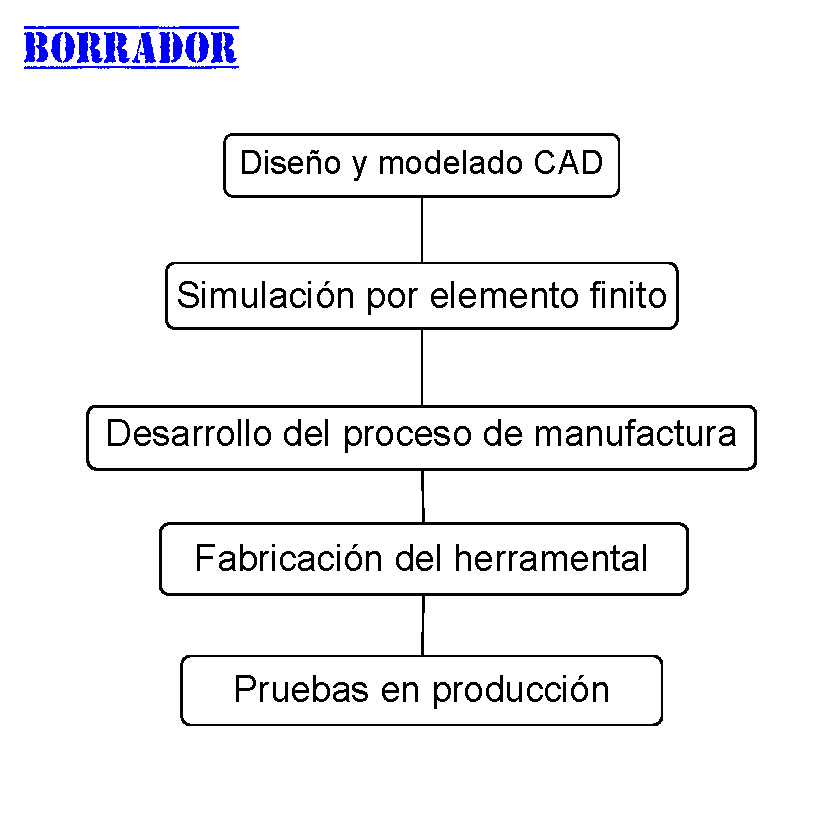
\includegraphics[width=0.75\textwidth]{src/ch3/diagrama_metodologia.pdf}
\captionof{figure}{Metodología del proyecto}
\label{fig:diagrama_metodologia}
\end{center}

\section{Consulta de fuentes de información}

En esta etapa inicial del proyecto se consultaron diversas fuentes de información 
relacionadas con los procesos de manufactura, específicamente los procesos 
de formado de hojas metálicas y operaciones de troquelado.

\section{Caracterización del material}

Cuando se requiere conocer las propiedades mecánicas de un material en ingeniería, se utilizan ensayos 
normalizados. En este caso se hace necesario obtener la curva esfuerzo-deformación del 
acero AISI 1018, misma que se utiliza como dato de entrada para la definición del material 
en el software de simulación utilizado. Para obtener el comportamiento esfuerzo-deformación 
de un metal se utiliza un ensayo de tensión uniaxial descrito en la norma ASTM-E8. ~\cite{ASTME8} \\

Del ensayo de tensión se obtuvieron los datos agrupados en la curva de la figura \ref{fig:material_curve}, 
en la cual se muestra, además, la curva esfuerzo-deformación verdadera calculada mediante las ecuaciones 
\ref{eq:true_stress} y \ref{eq:true_strain}.

\begin{center}
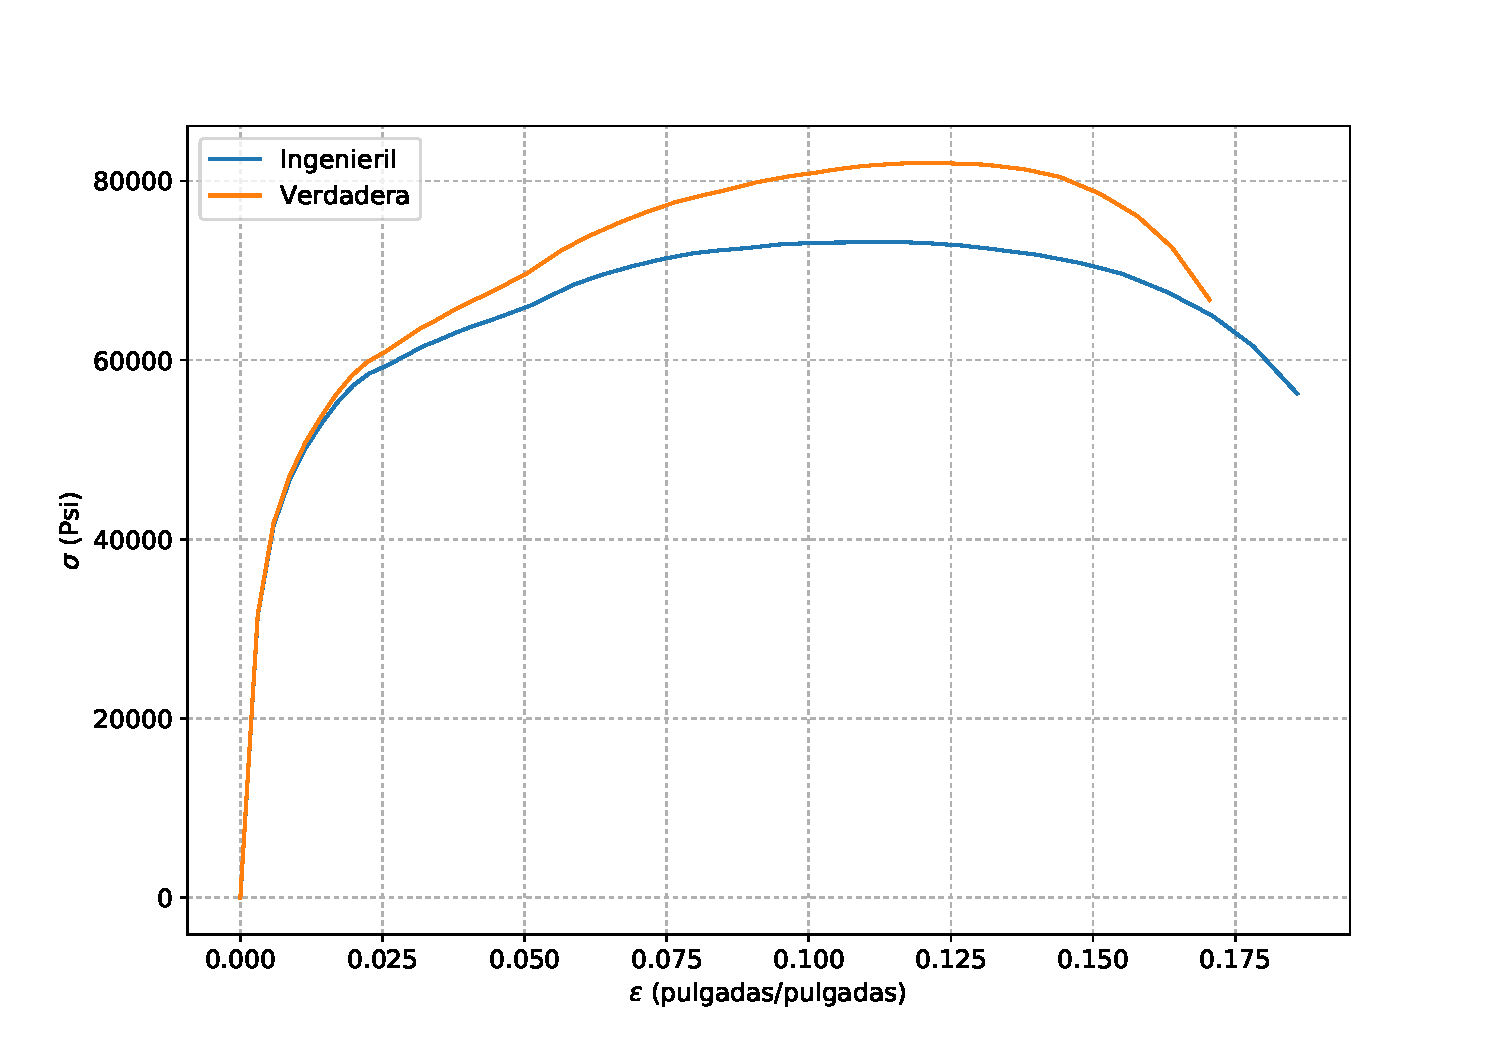
\includegraphics[scale=0.6]{src/ch3/material_curve.pdf}
\captionof{figure}{Curvas de esfuerzo-deformación, ingenieril y verdadera, del acero AISI 1018}
\label{fig:material_curve}
\end{center}

\section{Análisis por elementos finitos}

\begin{center}
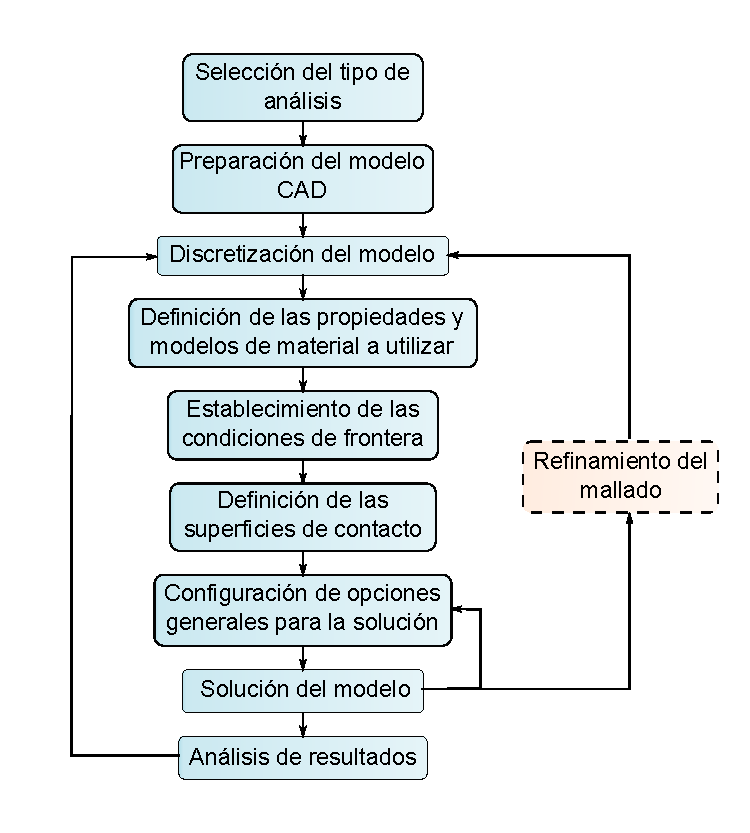
\includegraphics[width=0.75\textwidth]{src/ch3/metodologia_analisis_fem.pdf}
\captionof{figure}{Metodología para el análisis por elemento finito}
\label{fig:metodologia_analisis_fem}
\end{center}

\subsection{El proceso a simular}

En el capítulo \ref{ch:marco_de_referencia} se ha descrito someramente el proceso de formado que se requiere 
simular. Ahora, en lo subsiguiente, se detallan en mayor grado las características 
relativas al proceso, materiales utilizados y condiciones de operación que influyen en este. \\

El tubo interior mostrado en la figura \ref{fig:ti_rb131} se utiliza en un buje como 
el mostrado en la figura \ref{fig:buje_rb131}, el cual forma parte de un sistema de muelles 
parabólicas similar al de \ref{fig:muelle_parabolica}.

\begin{figure}[!h]
\centering
\begin{subfigure}[t]{0.35\textwidth}
\centering
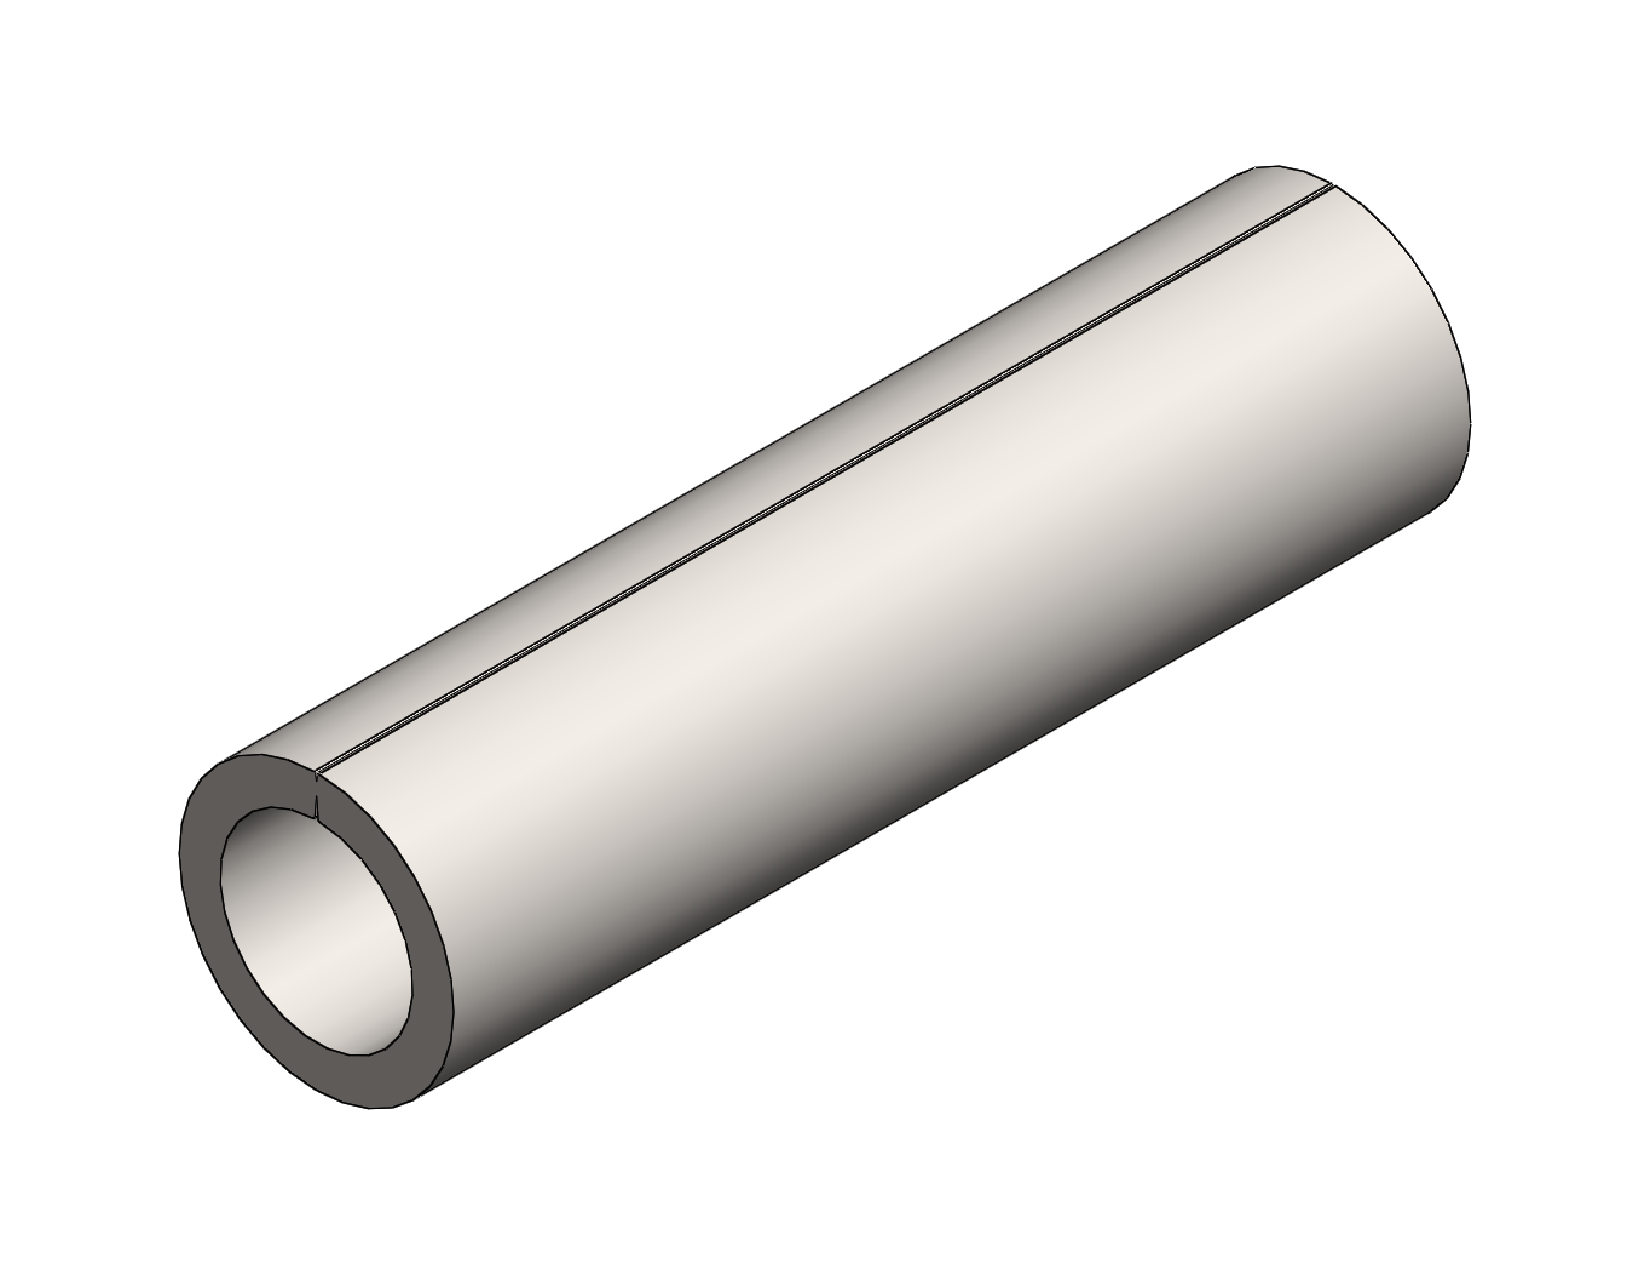
\includegraphics[width=\textwidth]{src/ch3/ti_rb131.pdf}
\caption{}
\label{fig:ti_rb131}
\end{subfigure}
~  
\begin{subfigure}[t]{0.35\textwidth}
\centering
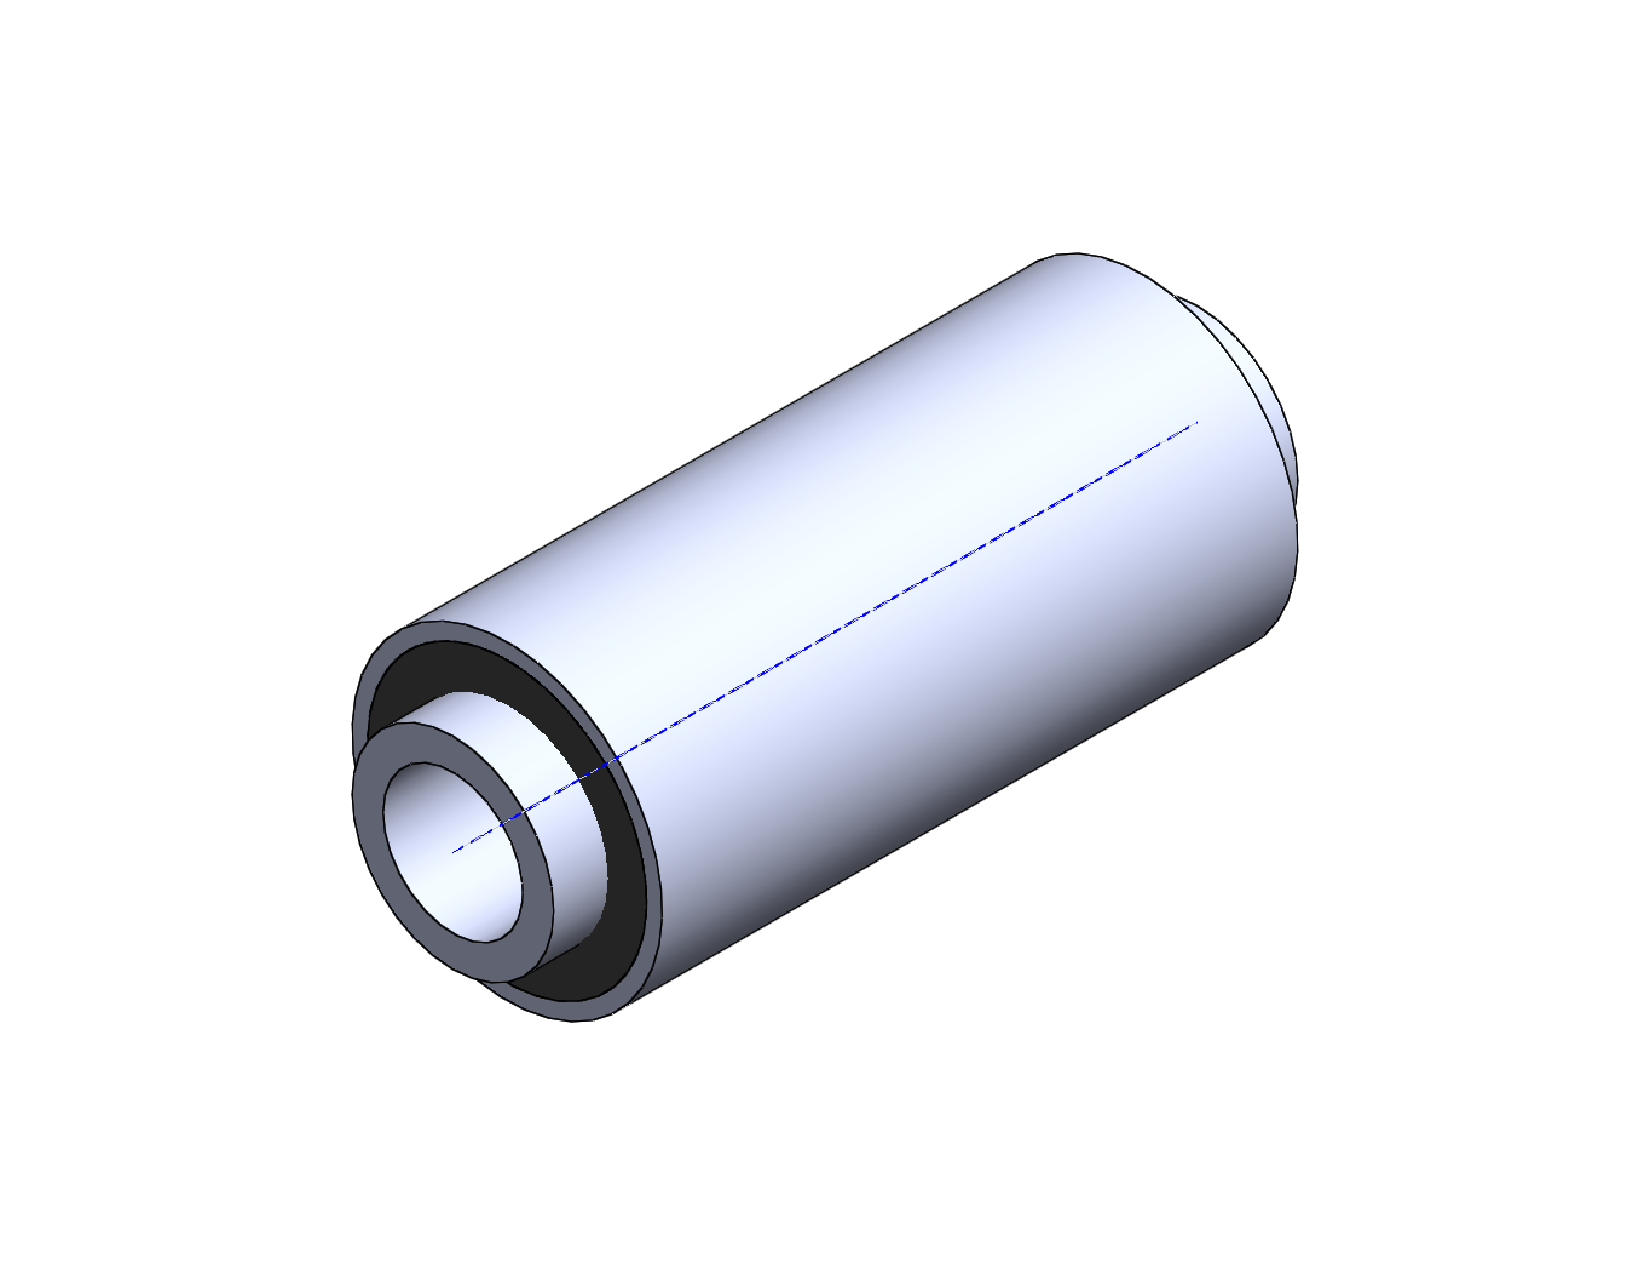
\includegraphics[width=\textwidth]{src/ch3/buje_rb131.pdf}
\caption{}
\label{fig:buje_rb131}
\end{subfigure}
\caption{a) Modelo CAD del tubo interior manufacturado por estampado b) Modelo CAD del buje RB-131}
\end{figure}


Para fabricar el tubo interior \ref{fig:ti_rb131} se utiliza un troquel compuesto o semiprogresivo 
de dos etapas, a saber: un doblado en U y un cerrado o doblado en O, mismo cuyo modelo CAD se muestra 
en la figura \ref{fig:troquel}. El troquel tiene como materia de entrada una placa metálica 
(\textit{blank}) rectangular de acero AISI 1018, con un largo de 3 in y un acho de 2.125 in, 
con un espesor de 0.12 in (ver figura \ref{fig:blank_inicial}). El \textif{blank} tiene además 
dos chaflanes en la dirección axial, sobre una de las caras, mismos que sirven para permitir un 
cierre de tubo adecuado.


\begin{center}
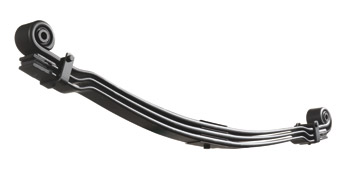
\includegraphics[scale=0.75]{src/ch3/muelle_parabolica.jpg}
\captionof{figure}{Muelle parabólica}
\label{fig:muelle_parabolica}
\end{center}


\begin{center}
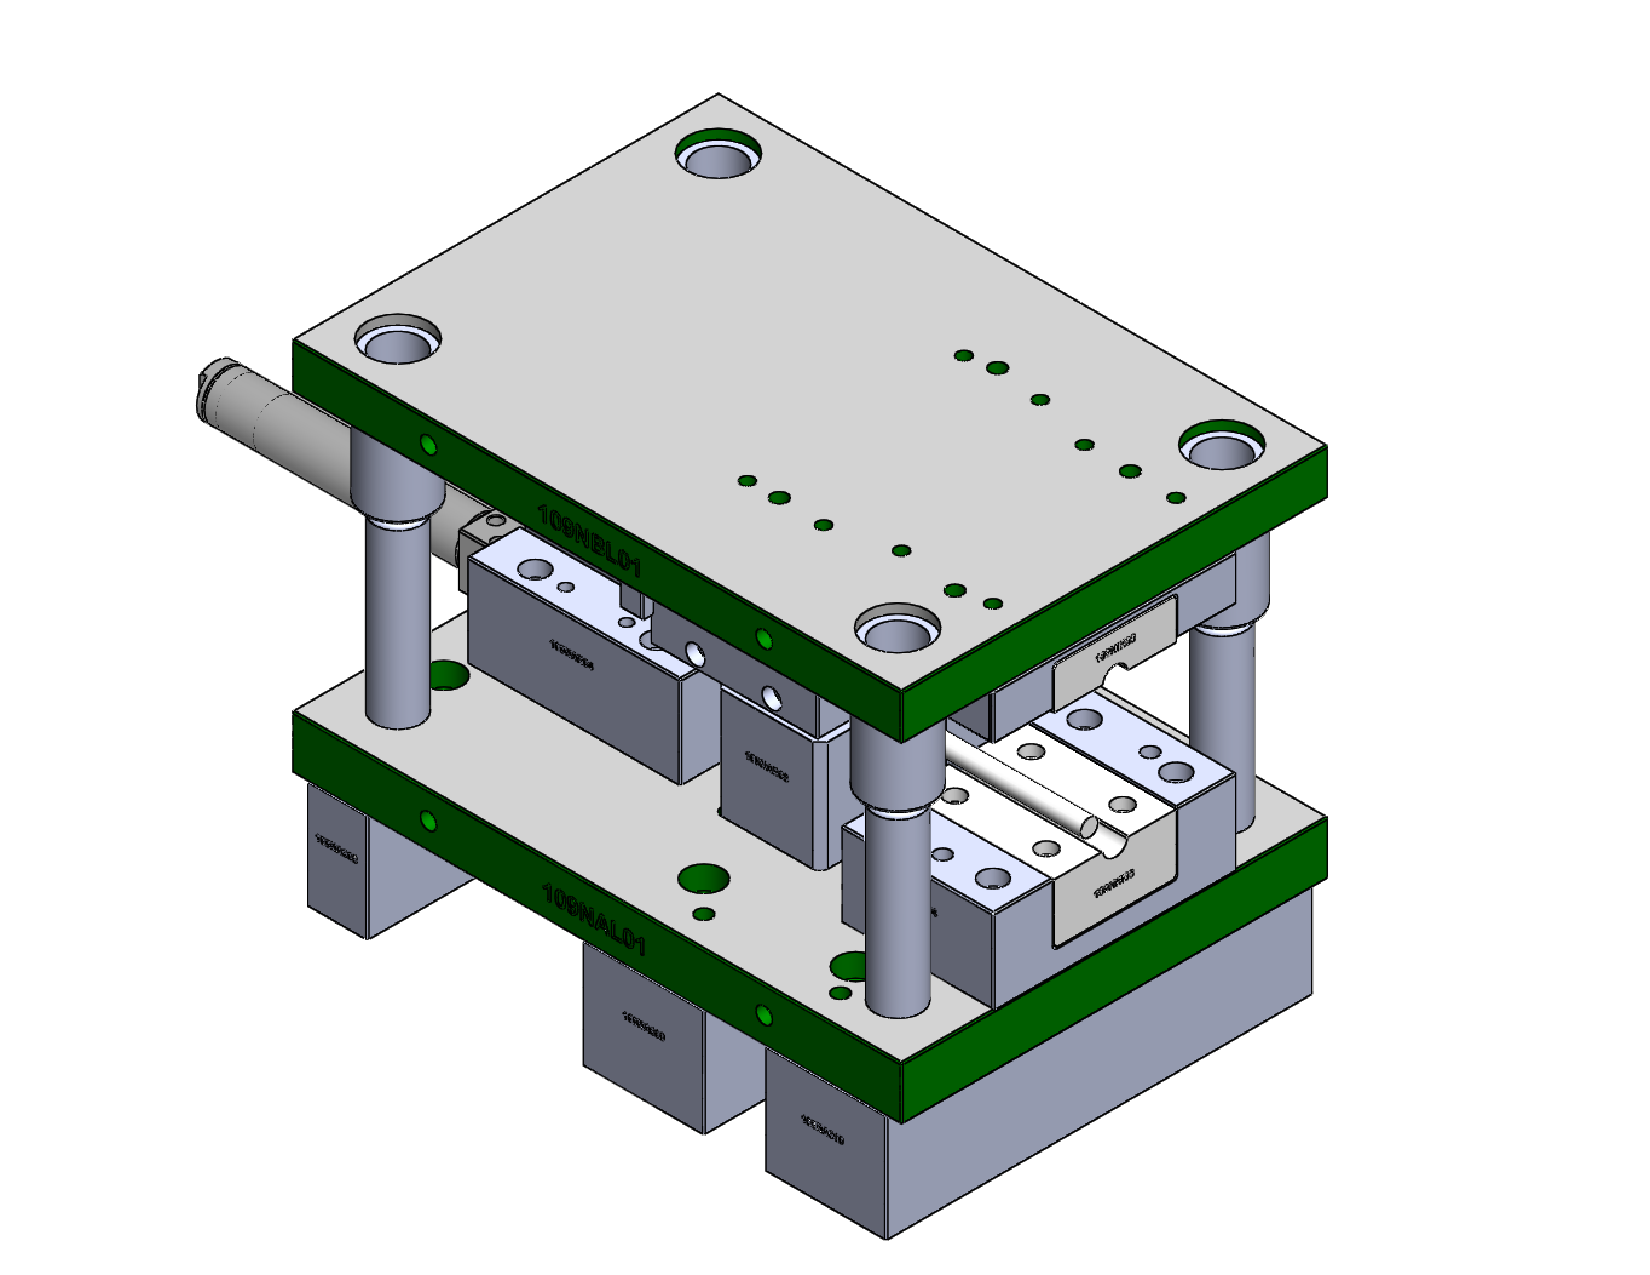
\includegraphics[scale=0.4]{src/ch3/troquel.pdf}
\captionof{figure}{Vista completa del troquel}
\label{fig:troquel}
\end{center}


\begin{figure}[!h]
\centering
\begin{subfigure}[t]{0.45\textwidth}
    \centering
    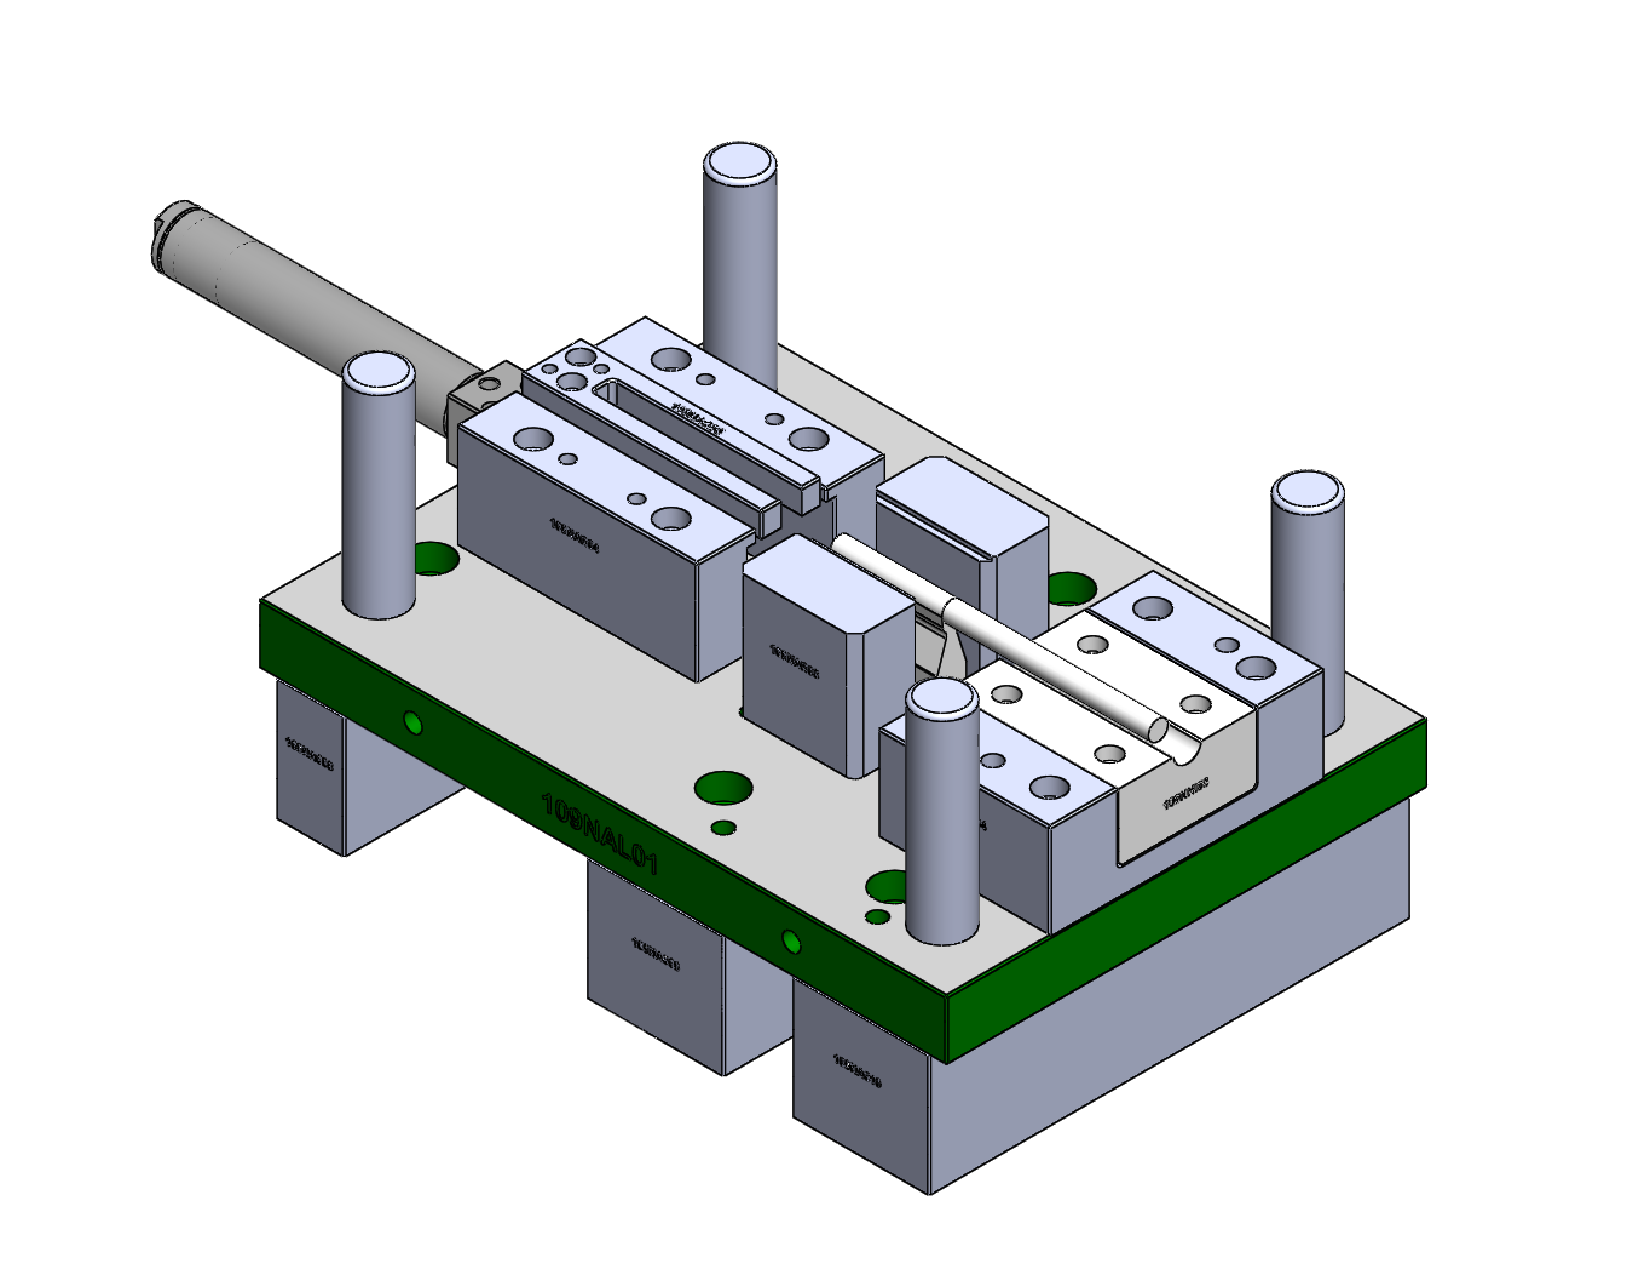
\includegraphics[width=\textwidth]{src/ch3/troquel_vista_inferior.pdf}
    \caption{}
    \label{fig:troquel_vista_inferior}
\end{subfigure}
~ 
\begin{subfigure}[t]{0.45\textwidth}
    \centering
    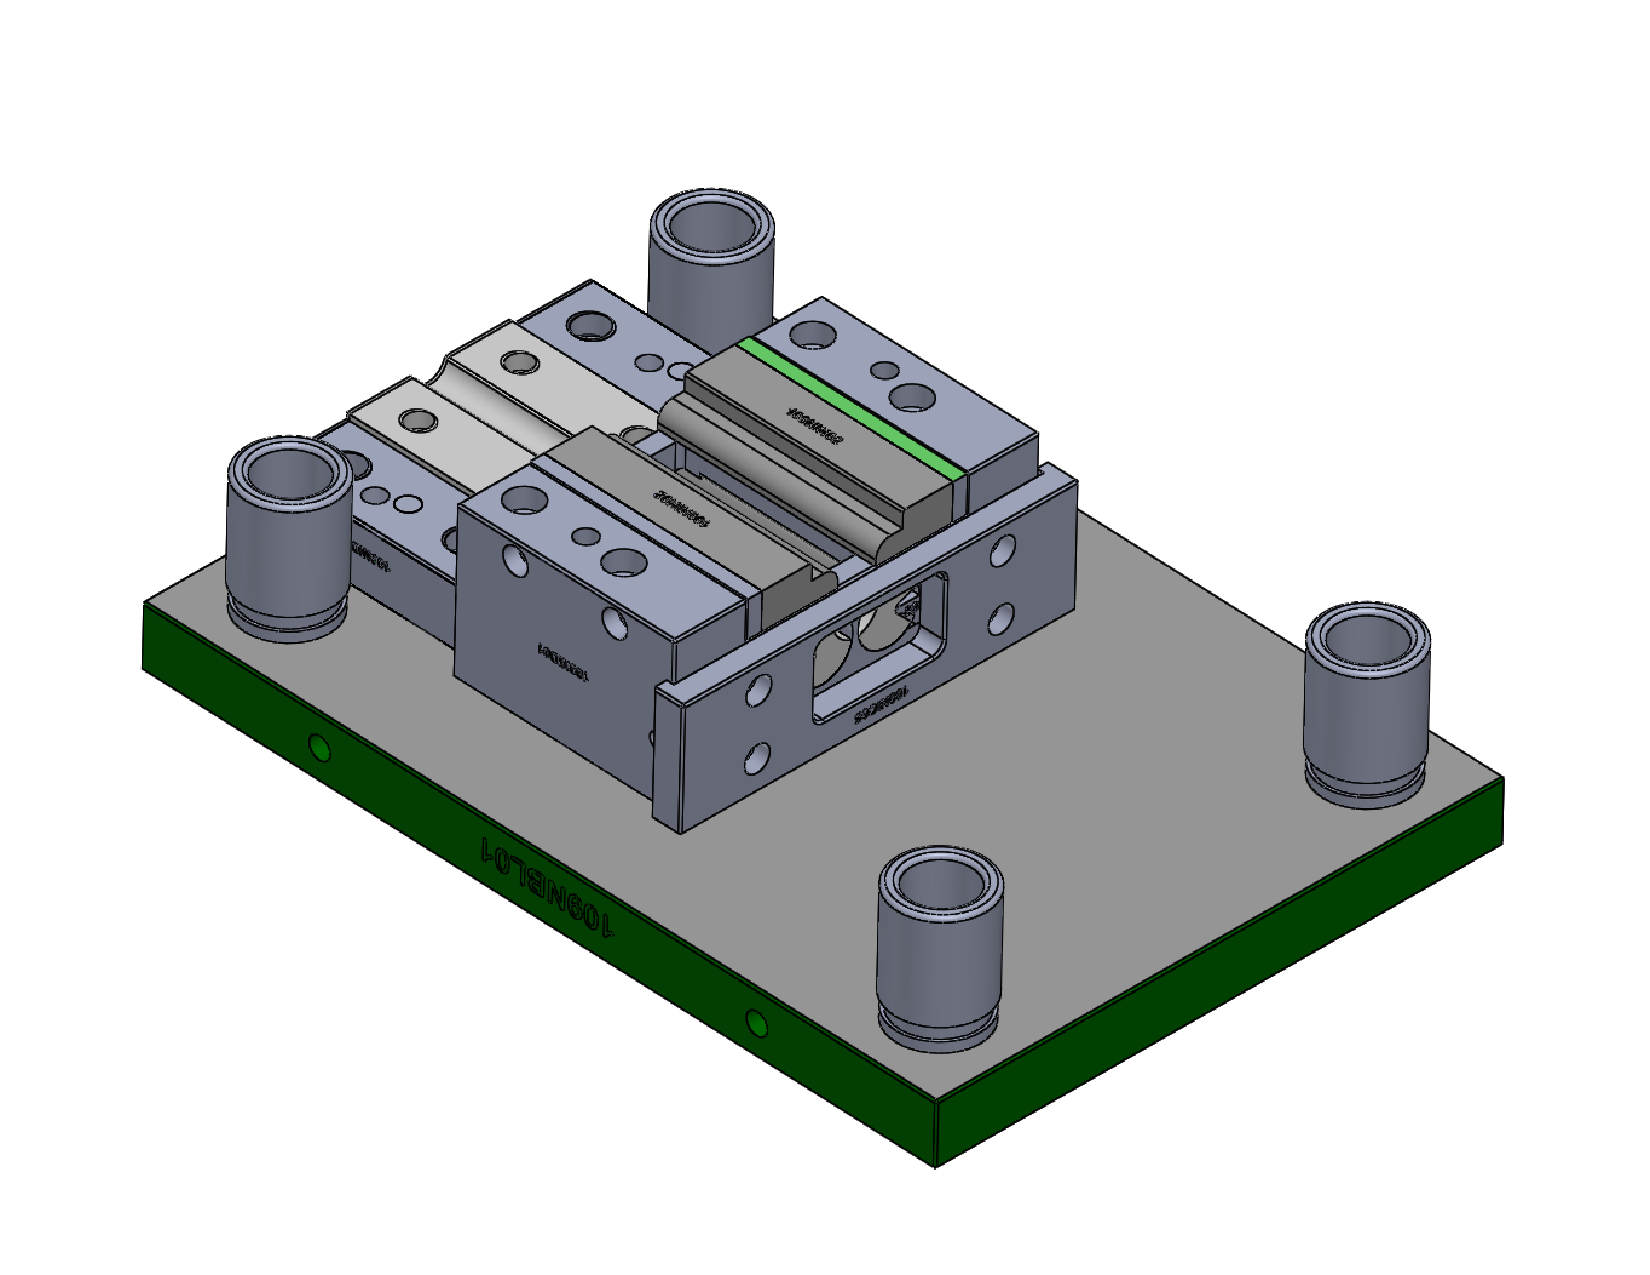
\includegraphics[width=\textwidth]{src/ch3/troquel_vista_superior.pdf}
    \caption{}
    \label{fig:troquel_vista_superior}
\end{subfigure}
\caption{Partes a) inferior y b) superior del troquel}

\end{figure}

\subsection{Generalidades de la simulación}



\subsection{Modelo constitutivo}

Para la pieza de trabajo se utilizó un modelo de tipo \textit{Piecewise Linear Plasticity}, 
el cual es un modelo multilineal que permite utilizar una curva esfuerzo-deformación y la 
dependencia de la tasa de deformación como datos de entrada para definir el comportamiento 
plástico del material. Para cuantificar la tasa de deformación este modelo utiliza la 
relación de Cowper-Symonds mostrada en la ecuación \ref{eq:cowper_symonds}.\\

\begin{equation} \label{eq:cowper_symonds}
\sigma_{y}\left( \varepsilon _{eff}^{P},\dot{\varepsilon }_{eff}^{P} \right) = 
{{\sigma }_{y}}\left( \varepsilon _{eff}^{P} \right)\left[ 1+{{\left( \frac{\dot{\varepsilon }_{eff}^{P}}{C} \right)}^{\frac{1}{P}}} \right]
\end{equation}

La curva esfuerzo-deformación ingresada en el software de simulación fue la obtenida 
de forma experimental, con algunas modificaciones a saber: se tomaron solamente 7 puntos 
de la curva original linealmente equiespaciados, se calculó el esfuerzo y deformación verdadera 
mediante las ecuaciones descritas en la sección \ref{subsec:true_strain_stress}, posteriormente 
a partir de la deformación verdadera se obtuvo la deformación plástica mediante la 
ecuación \ref{eq:plastic_strain}, mismas que se agrupan en la tabla \ref{tab:strain_stress_conversion}.
La curva resultante y que se ingresó en el softaware se muestra en la figura \ref{fig:ls_dyna_material_curve}. \\

Para definir completamente el modelo es necesario asignar las propiedades mecánicas elementales 
como el módulo elástico, la relación de Poisson y la densidad. Además, se debe asignar 
la resistencia a la fluencia y las constantes C y P utilizadas en la ecuación de Cowper-Symonds.
Estas propiedades utilizadas se muestran en la tabla \ref{tab:material_properties}. \\

% Tabla de propiedades
\begin{table}[h]
\centering
\caption{Propiedades del acero AISI 1018}
\label{tab:steel_properties}
\begin{tabular}{p{4cm} p{4cm}} \hline
Propiedad & Magnitud (unidades) \\
\hline
Módulo elástico & 29 000 (ksi) \\
Densidad & 0.00073 (lbf s$^2$/in$^4$) \\
Esfuerzo de fluencia & 52 000 (psi) \\
Coeficiente de Poisson & 0.3 \\
C & 40 (s$^{-1}$) \\
P & 5 \\
\hline
\end{tabular}
\label{tab:material_properties}
\end{table}

En los componentes del troquel se utilizó un modelo rígido, para el cual sólo es necesario 
especificar las propiedades elásticas. Los componentes rígidos, normalmente, permiten la 
aplicación de condiciones de desplazamiento utilizando el identificador o ID de la parte, además 
se pueden asignar propiedades de inercia o velocidades iniciales. En este caso, no se 
especificaron propiedades adicionales, lo cual implica que el software de simulación calcule automáticamente 
las propiedades inerciales basadas en el modelo de elemento finito. \\

Para crear los materiales de cada uno de los componentes se utilizó un pequeño \textit{script}, 
que se muestra a continuación:,k

\begin{apdl}
! Para el formador inferior
MP,EX,2,29E6 ! psi
MP,NUXY,2,0.3 ! 
MP,DENS,2,0.00073 ! lbf s^2 / in^4
EDMP,rigid,2,7,7

! Formador superior izquierdo
MP,EX,3,29E6 ! psi
MP,NUXY,3,0.3 ! 
MP,DENS,3,0.00073 ! lbf s^2 / in^4
EDMP,rigid,3,6,7

! Formador superior derecho
MP,EX,4,29E6 ! psi
MP,NUXY,4,0.3 ! 
MP,DENS,4,0.00073 ! lbf s^2 / in^4
EDMP,rigid,4,6,7

! Leva izquierda
MP,EX,5,29E6 ! psi
MP,NUXY,5,0.3 ! 
MP,DENS,5,0.00073 ! lbf s^2 / in^4
EDMP,rigid,5,6,4

! Leva derecha
MP,EX,6,29E6 ! psi
MP,NUXY,6,0.3 ! 
MP,DENS,6,0.00073 ! lbf s^2 / in^4
EDMP,rigid,6,6,4

! Para el blank
! Propiedades elásticas
MP,EX,1,29E6 ! psi
MP,NUXY,1,0.3 ! 
MP,DENS,1,0.00073 ! lbf s^2 / in^4

! Definir un arreglo para la deformación plástica verdadera
*dim,strn,,6
! Definir un arreglo para el esfuerzo verdadero
*dim,strs,,6

! Deformación (in/in)
strn(1) = 0.0, 0.0293, 0.0772, 0.1562, 0.2356, 0.344943

! Esfuerzo (psi)
strs(1) = 52489.4,60585.8,70710,76809.3,80244.3,82574.1

! Curva #1: Abscisa=deformación & Ordenada=esfuerzo
edcurve,add,1,strn,strs 

! Especificar Power Law #8 para el material #1
TB,PLAW,1,,,8  ! Piecewise Linear Plasticity

! Usar curva #1 para la relación esfuerzo-deformación
TBDATA,1,52e3 ! Esfuerzo de fluencia (psi)
TBDATA,3,.75 ! Deformación de falla
TBDATA,4,40.0 ! C (Parámetro de tasa de deformación)
TBDATA,5,0.1 ! P (Parámetro de tasa de deformación)
TBDATA,6,1 ! ID de la curva
\end{apdl}


% Tabla de propiedades plásticas

\begin{table}[h]
\centering
\caption{Conversión de esfuerzos y deformaciones}
\label{tab:strain_stress_conversion}
\begin{tabular}{p{2.5cm} p{2.5cm} p{2.5cm} p{2.5cm} p{2.5cm}} \hline
{\bf $\varepsilon_{nom}$ & $\sigma_{nom}$ (psi) & $\varepsilon_t$ & $\sigma_t$ (psi) & $\varepsilon_{pl}$ } \\
\hline
0.0084 & 51376.41 & 0.0084 & 51808.49 & 0.0000 \\
0.0224 & 59624.27 & 0.0221 & 60957.47 & 0.0200 \\
0.0418 & 67059.05 & 0.0409 & 69858.77 & 0.0385 \\
0.0607 & 70769.55 & 0.0589 & 75063.85 & 0.0563 \\
0.0846 & 72814.73 & 0.0812 & 78971.94 & 0.0785 \\
0.1287 & 72924.09 & 0.1210 & 82305.77 & 0.1182 \\
0.1554 & 70462.94 & 0.1444 & 81412.18 & 0.1416 \\
\hline
\end{tabular}
\label{tab:stress_strain_curve}
\end{table}


\begin{center}
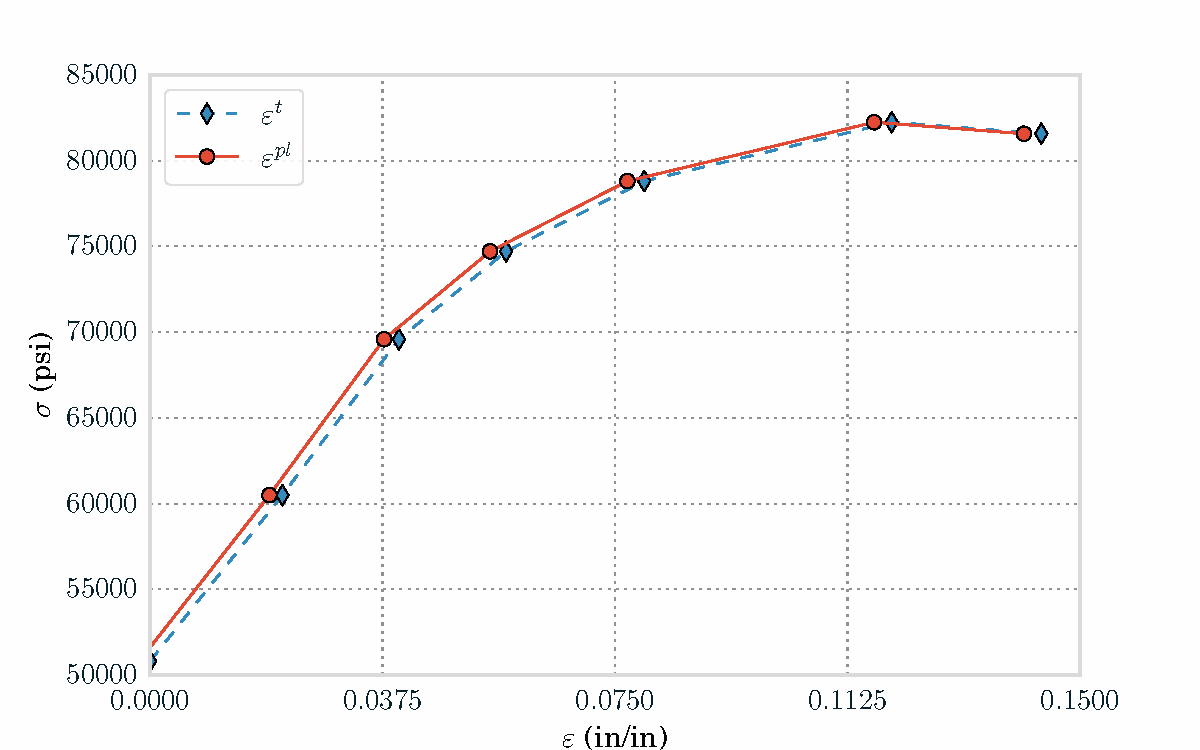
\includegraphics[scale=0.6]{src/ch3/ls_dyna_material_curve.pdf}
\captionof{figure}{Curva esfuerzo-deformación ingresada en ANSYS/LS-DYNA}
\label{fig:ls_dyna_material_curve}
\end{center}


\subsection{Mallado}

\subsubsection{Primer ensamble}

Para el mallado de la pieza de trabajo se utilizó el elemento \texttt{SOLID164} 
( ver figura \ref{fig:solid164} ), el cual es un sólido de 8 nodos, que puede ser utilizado con el modelo 
constitutivo descrito en la sección anterior. Este elemento utiliza, por defecto, integración reducida 
(un punto de integración), el cual tiene la ventaja de reducir el tiempo de cómputo y adiciona 
robustez para el caso de grandes deformaciones ~\cite{lsdyna-ansys-manual}, no obstante puede presentar 
la desventaja de propiciar la inclusión de los modos de Hourglass en la solución, implicando que 
se obtenga una malla deformada con apariencia corrugada.

\begin{center}
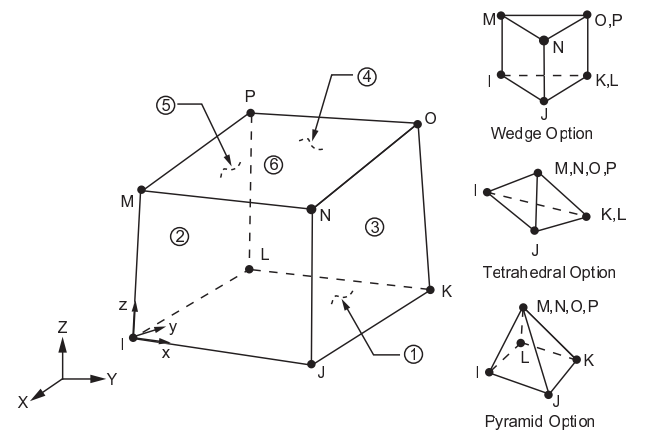
\includegraphics[scale=0.65]{src/ch3/solid164.png}
\captionof{figure}{Elemento \texttt{SOLID164}}
\label{fig:solid164}
\end{center}

En los componentes del troquel se mallaron solamente las áreas que están en contacto directo con el 
\textit{blank} durante el proceso de formado, con la finalidad de reducir el número de elementos del modelo. 
Se utilizaron elementos \texttt{SHELL163} para realizar el mallado. Los parámetros requeridos para 
este elemento se indican en la tabla \ref{tab:shell_param}.

\begin{center}
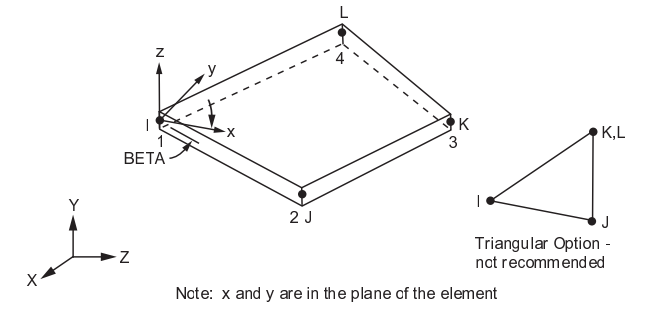
\includegraphics[scale=0.65]{src/ch3/shell163.png}
\captionof{figure}{Elemento SHELL163}
\label{fig:shell163}
\end{center}


% Tabla de propiedades para elemento SHELL163
\begin{table}[h]
\centering
\caption{Parámetros utilizados para el elemento SHELL163}
\label{}
\begin{tabular}{p{6cm} p{6cm}} \hline
Parámetros & Valores \\
\hline
General shell formulation & Belytschko-Tsay \\
Membrane element formulation & Belytschko-Tsay Membrane \\
Triangular shell formulation & $C^0$ triangular shell \\
\hline
\end{tabular}
\label{tab:shell_param}
\end{table}


% Tabla de constantes reales para elemento SHELL163
\begin{table}[h]
\centering
\caption{Constantes reales para el elemento SHELL163}
\label{}
\begin{tabular}{p{6cm} p{3cm}} \hline
Parámetros & Valores \\
\hline
Factor cortante (SHRF) & 5/6 \\
Puntos de integración (NIP) & 1 \\
Espesor en nodo 1 (T1) & 0.2 \\
Espesor en nodo 2 (T2) & 0.2 \\
Espesor en nodo 3 (T3) & 0.2 \\
Espesor en nodo 4 (T4) & 0.2 \\
\hline
\end{tabular}
\label{tab:shell_param}
\end{table}


En el \textit{blank} se utilizó un tamaño global de elemento de 0.03 in, y 0.035 in en el caso de las partes 
rígidas, exceptuando las áreas que están directamente en contacto con el \textit{blank}, en cuyo caso se hizo 
un refinamiento, dejando el tamaño global en 0.02 in. En el \textit{blank} fue necesario segmentar en cuatro 
volúmenes, para permitir un mallado más uniforme (ver figura \ref{fig:blank_seg} ).


% Partición del blank
\begin{center}
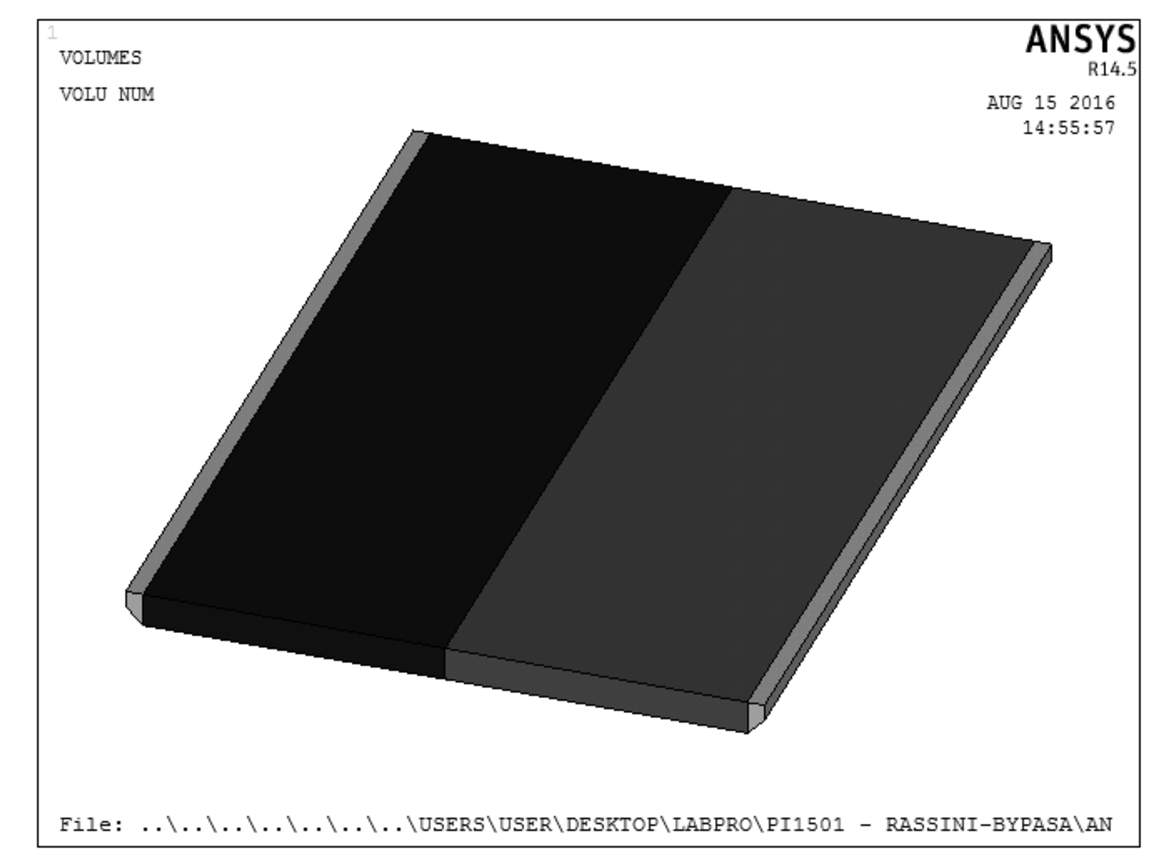
\includegraphics[width=0.5\textwidth]{src/ch3/blank_segmentado.pdf}
\captionof{figure}{Blank segmentado en cuatro regiones}
\label{fig:blank_seg}
\end{center}


% Mallado del blank


\begin{figure}[!h]
\centering
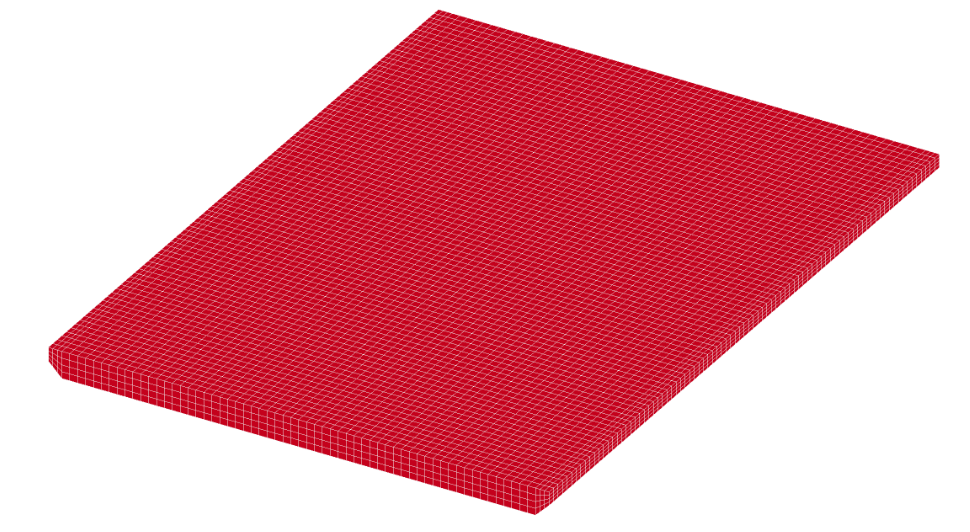
\includegraphics[width=0.5\textwidth]{src/ch3/mesh_blank.png}
\label{fig:mesh_blank}
\caption{Mallado del blank}
\end{figure}


\begin{figure}[!h]
\centering
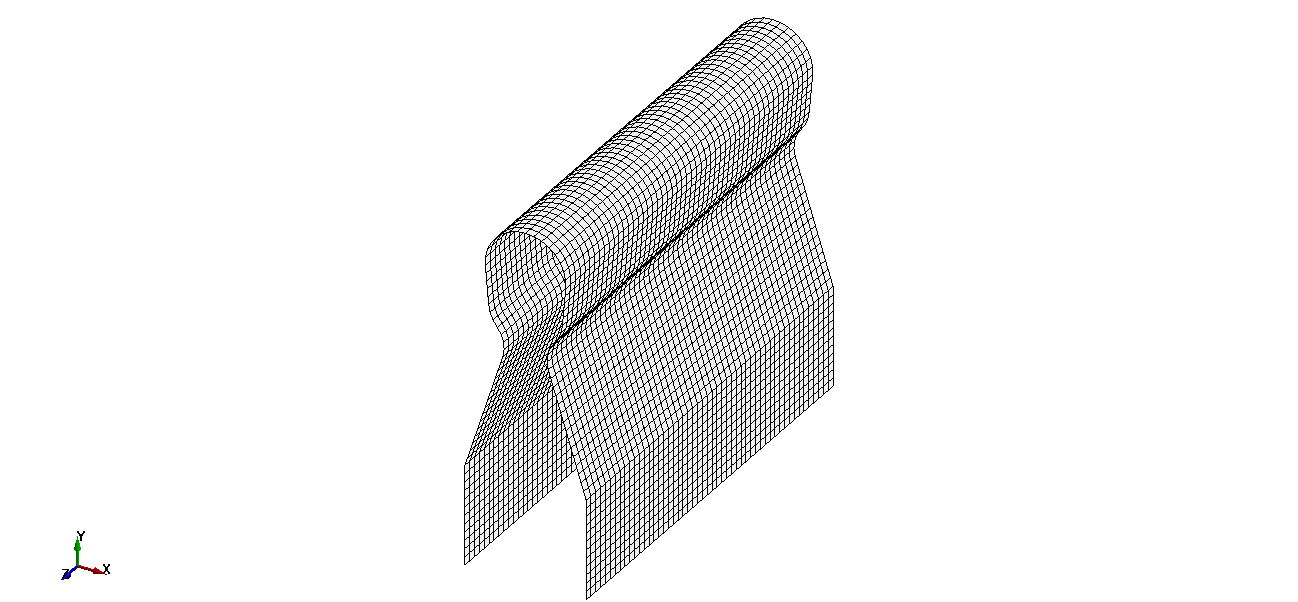
\includegraphics[width=0.5\textwidth]{src/ch3/mesh_fi.png}
\caption{Mallado del formador inferior}
\label{fig:mesh_fi}
\end{figure}

\begin{figure}[!h]
\centering
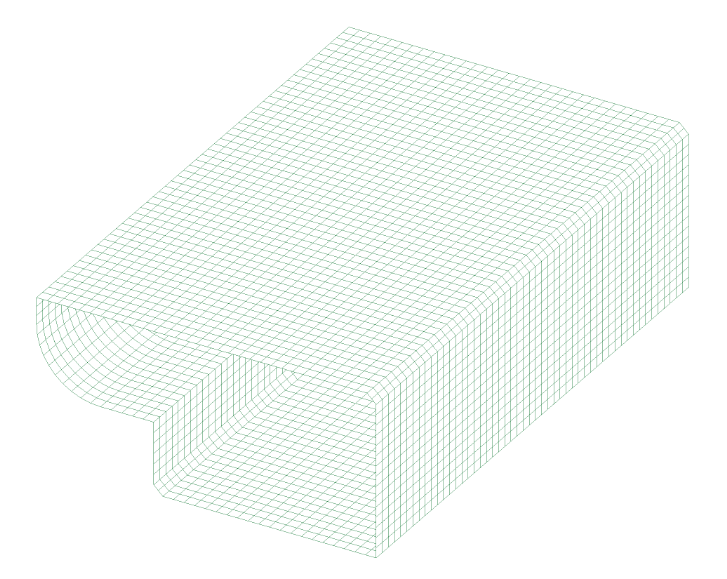
\includegraphics[width=0.5\textwidth]{src/ch3/mesh_fs.png}
\caption{Mallado del formador superior}
\label{fig:mesh_fi}
\end{figure}

\begin{figure}[!h]
\centering
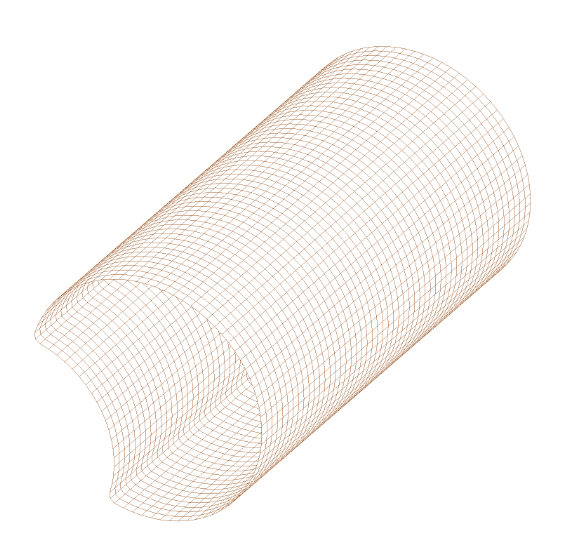
\includegraphics[width=0.5\textwidth]{src/ch3/mesh_leva.png}
\caption{Mallado de la leva}
\label{fig:mesh_fi}
\end{figure}


% \begin{figure}[!h]
% \centering
% \begin{subfigure}[t]{0.3\textwidth}
% \centering
% 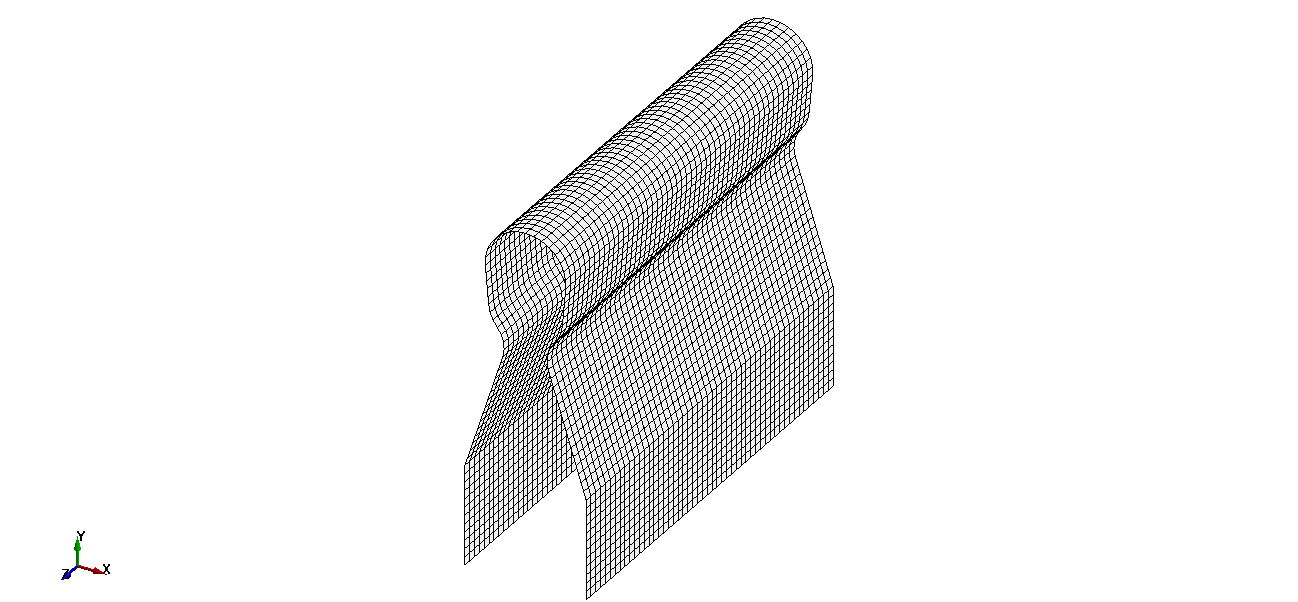
\includegraphics[width=\textwidth]{src/ch3/mesh_fi.png}
% \caption{}
% \label{fig:mesh_fi}
% \end{subfigure}
% ~ 
% \begin{subfigure}[t]{0.3\textwidth}
% \centering
% 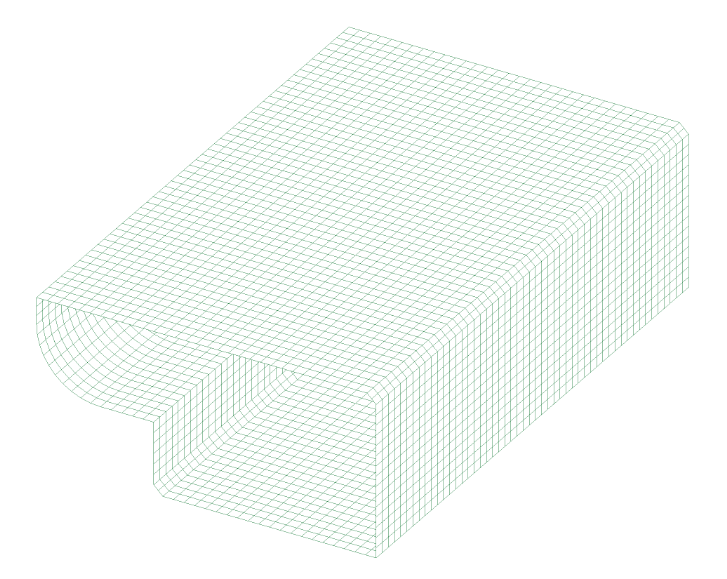
\includegraphics[width=\textwidth]{src/ch3/mesh_fs.png}
% \caption{}
% \label{fig:mesh_fs}
% \end{subfigure}
% ~ 
% \begin{subfigure}[t]{0.3\textwidth}
% \centering
% 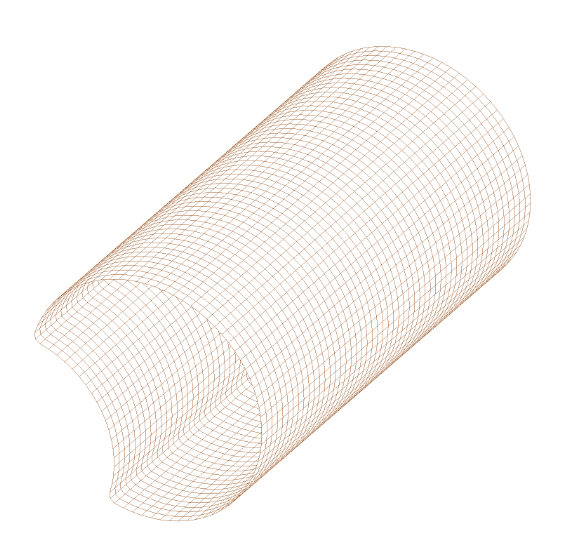
\includegraphics[width=\textwidth]{src/ch3/mesh_leva.png}
% \caption{}
% \label{fig:mesh_leva}
% \end{subfigure}

% \caption{Mallado de a) formador inferior b) formador superior c) leva}
% \end{figure}


%  Partes 
\begin{figure}[!h]
\centering
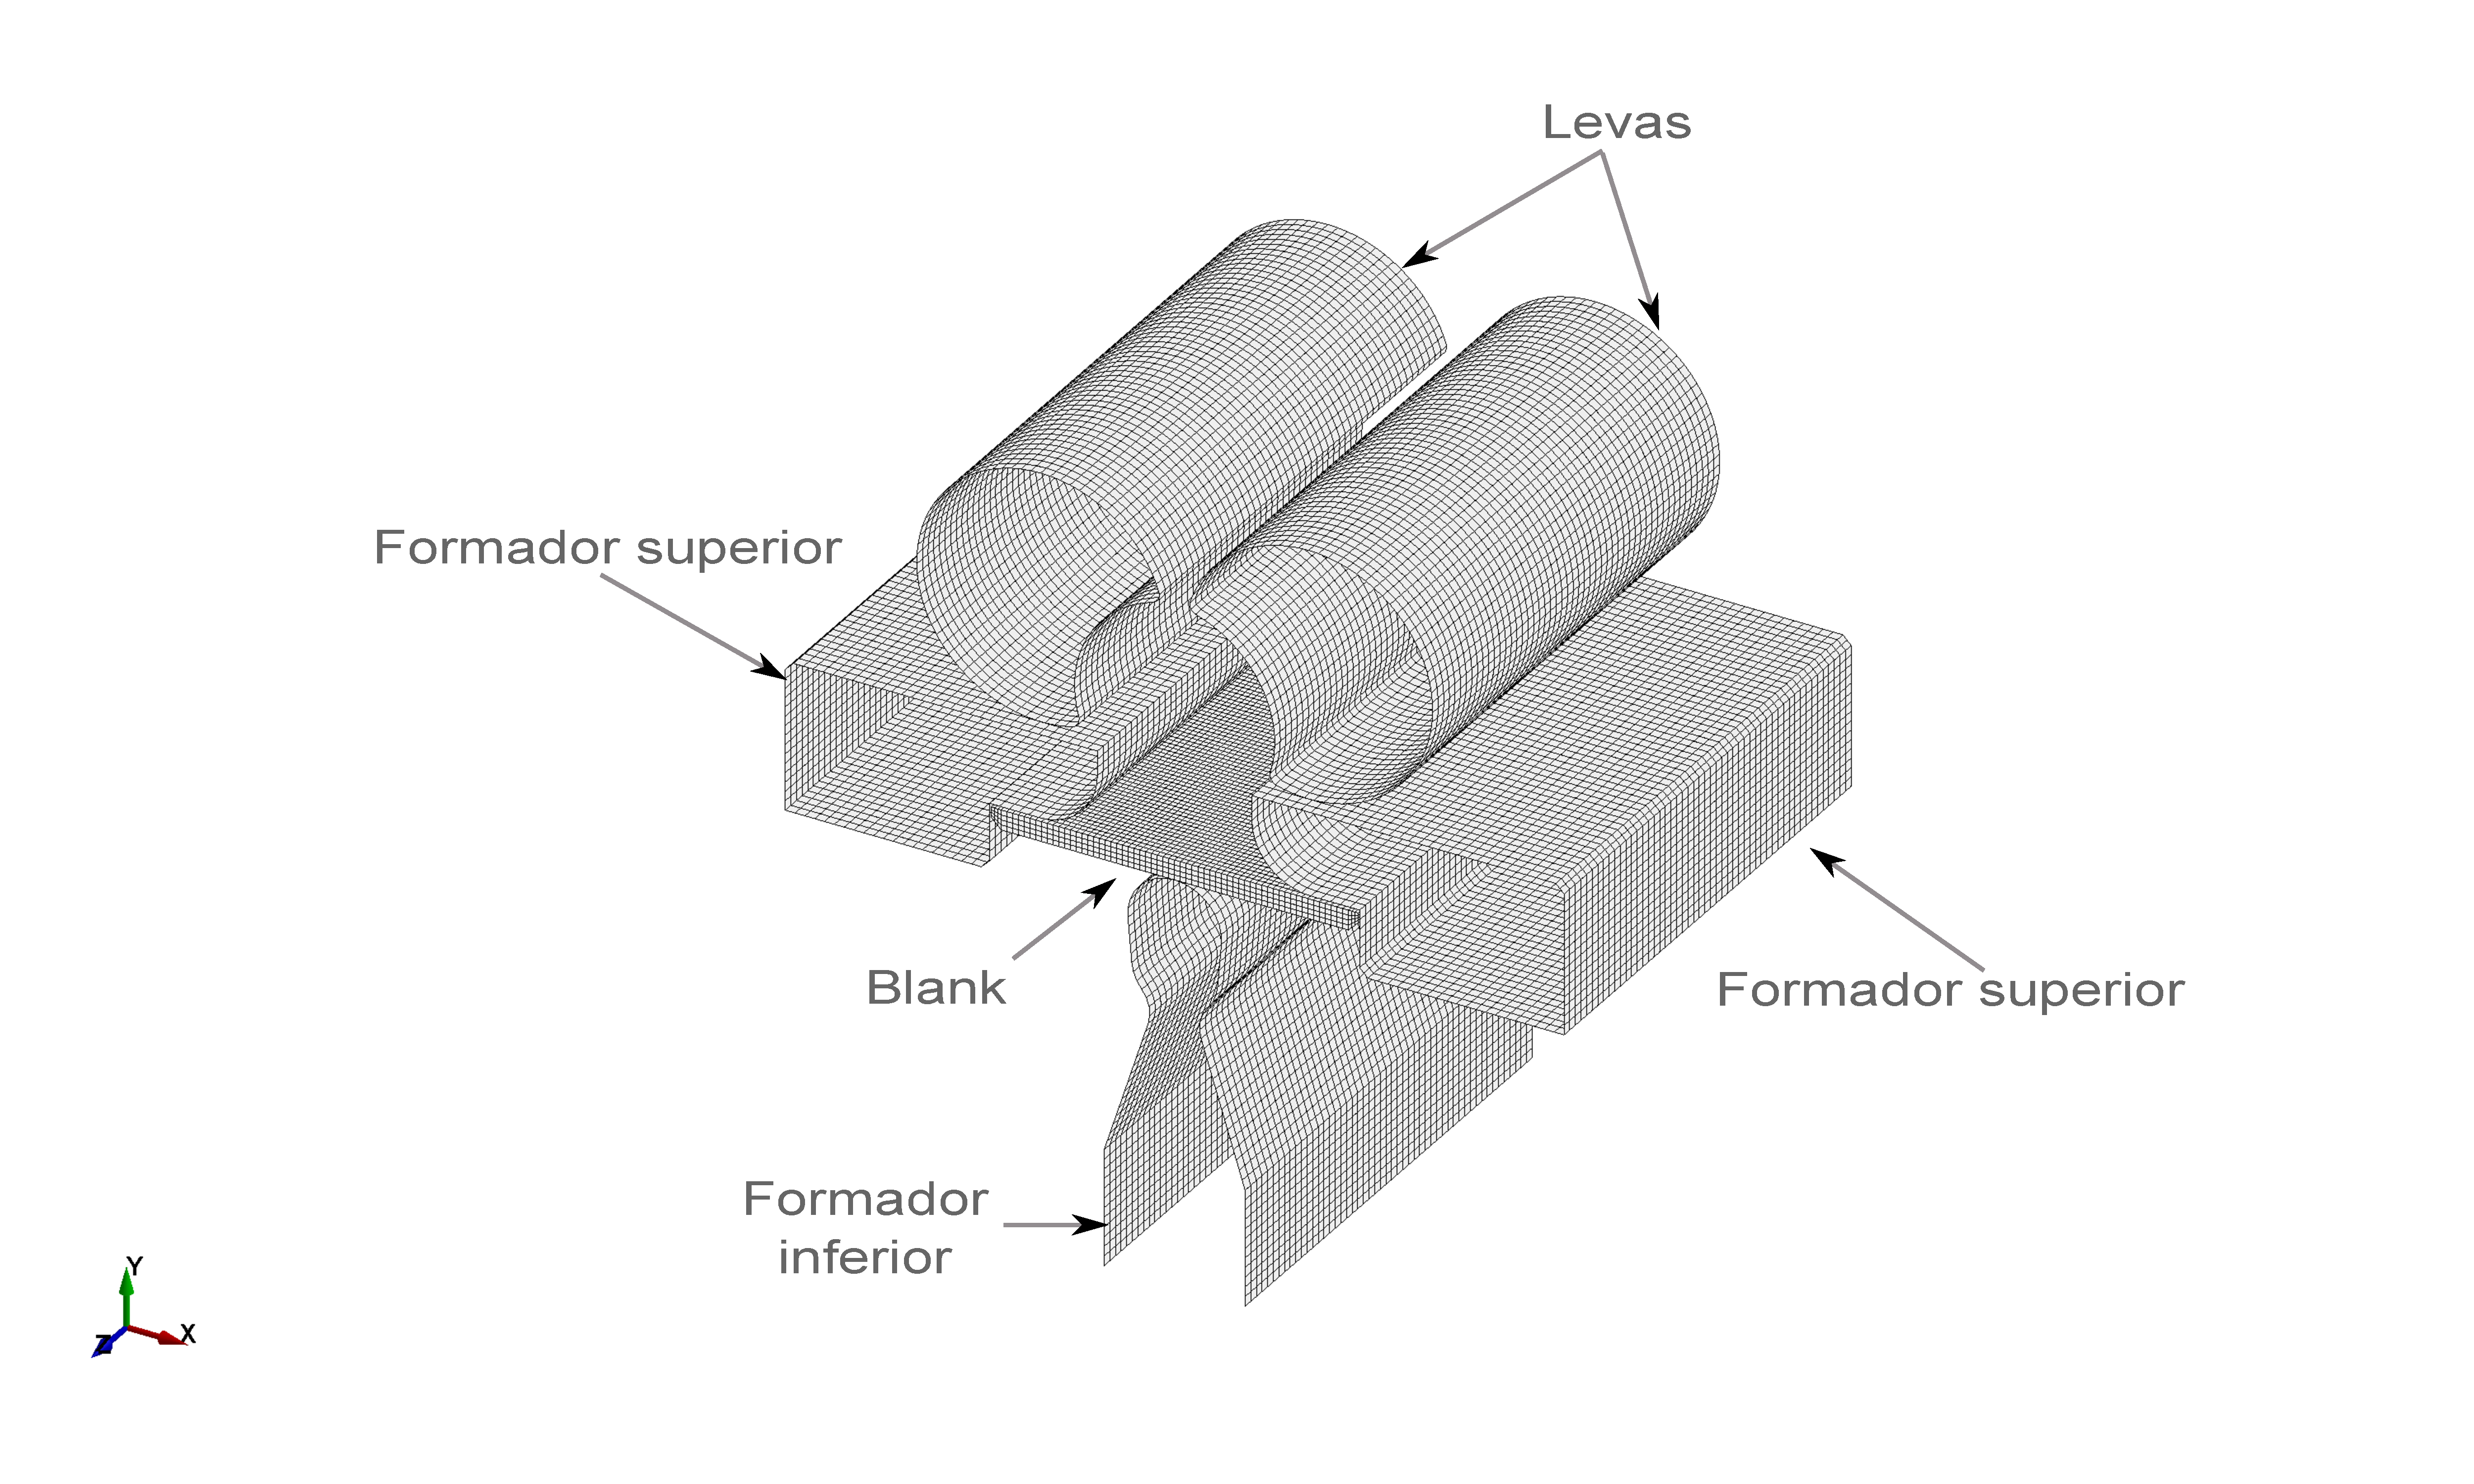
\includegraphics[width=0.8\textwidth]{src/ch3/parts_01.pdf}
\caption{Partes del ensamble 1}
\label{fig:parts_01}
\end{figure}

% En las tabla \ref{tab:elements_and_nodes} se muestra el número de nodos y elementos obtenidos 
% para cada uno de los ensambles.

% \begin{table}[h]
% \centering
% \caption{Número de nodos y elementos}
% \label{}
% \begin{tabular}{p{2cm} p{2cm} p{2cm}} \hline
%  & Nodos & Elementos \\
% \hline
% Paso 1 & 52285 & 45348 \\
% Paso 2 & 48884 & 42264 \\
% \hline
% \end{tabular}
% \label{tab:elements_and_nodes}
% \end{table}


\subsubsection{Segundo ensamble}

Al igual que en el primer ensamble, los formadores y/o componentes del herramental, se 
mallaron por áreas utilizando elementos \texttt{SHELL163}. En el caso de la pieza de trabajo, 
esta se importó en su configuración deformada del análisis del primer paso, incluyendo 
además la distribución de esfuerzos. En la figura \ref{fig:mesh_blank_02} se observa 
la malla deformada del blank. El mallado de cada uno de los componentes del troquel 
se puede observar en las figuras \ref{fig:mesh_ffi}, \ref{fig:mesh_ffs} y \ref{fig:mesh_perno}.


\begin{figure}[!h]
\centering
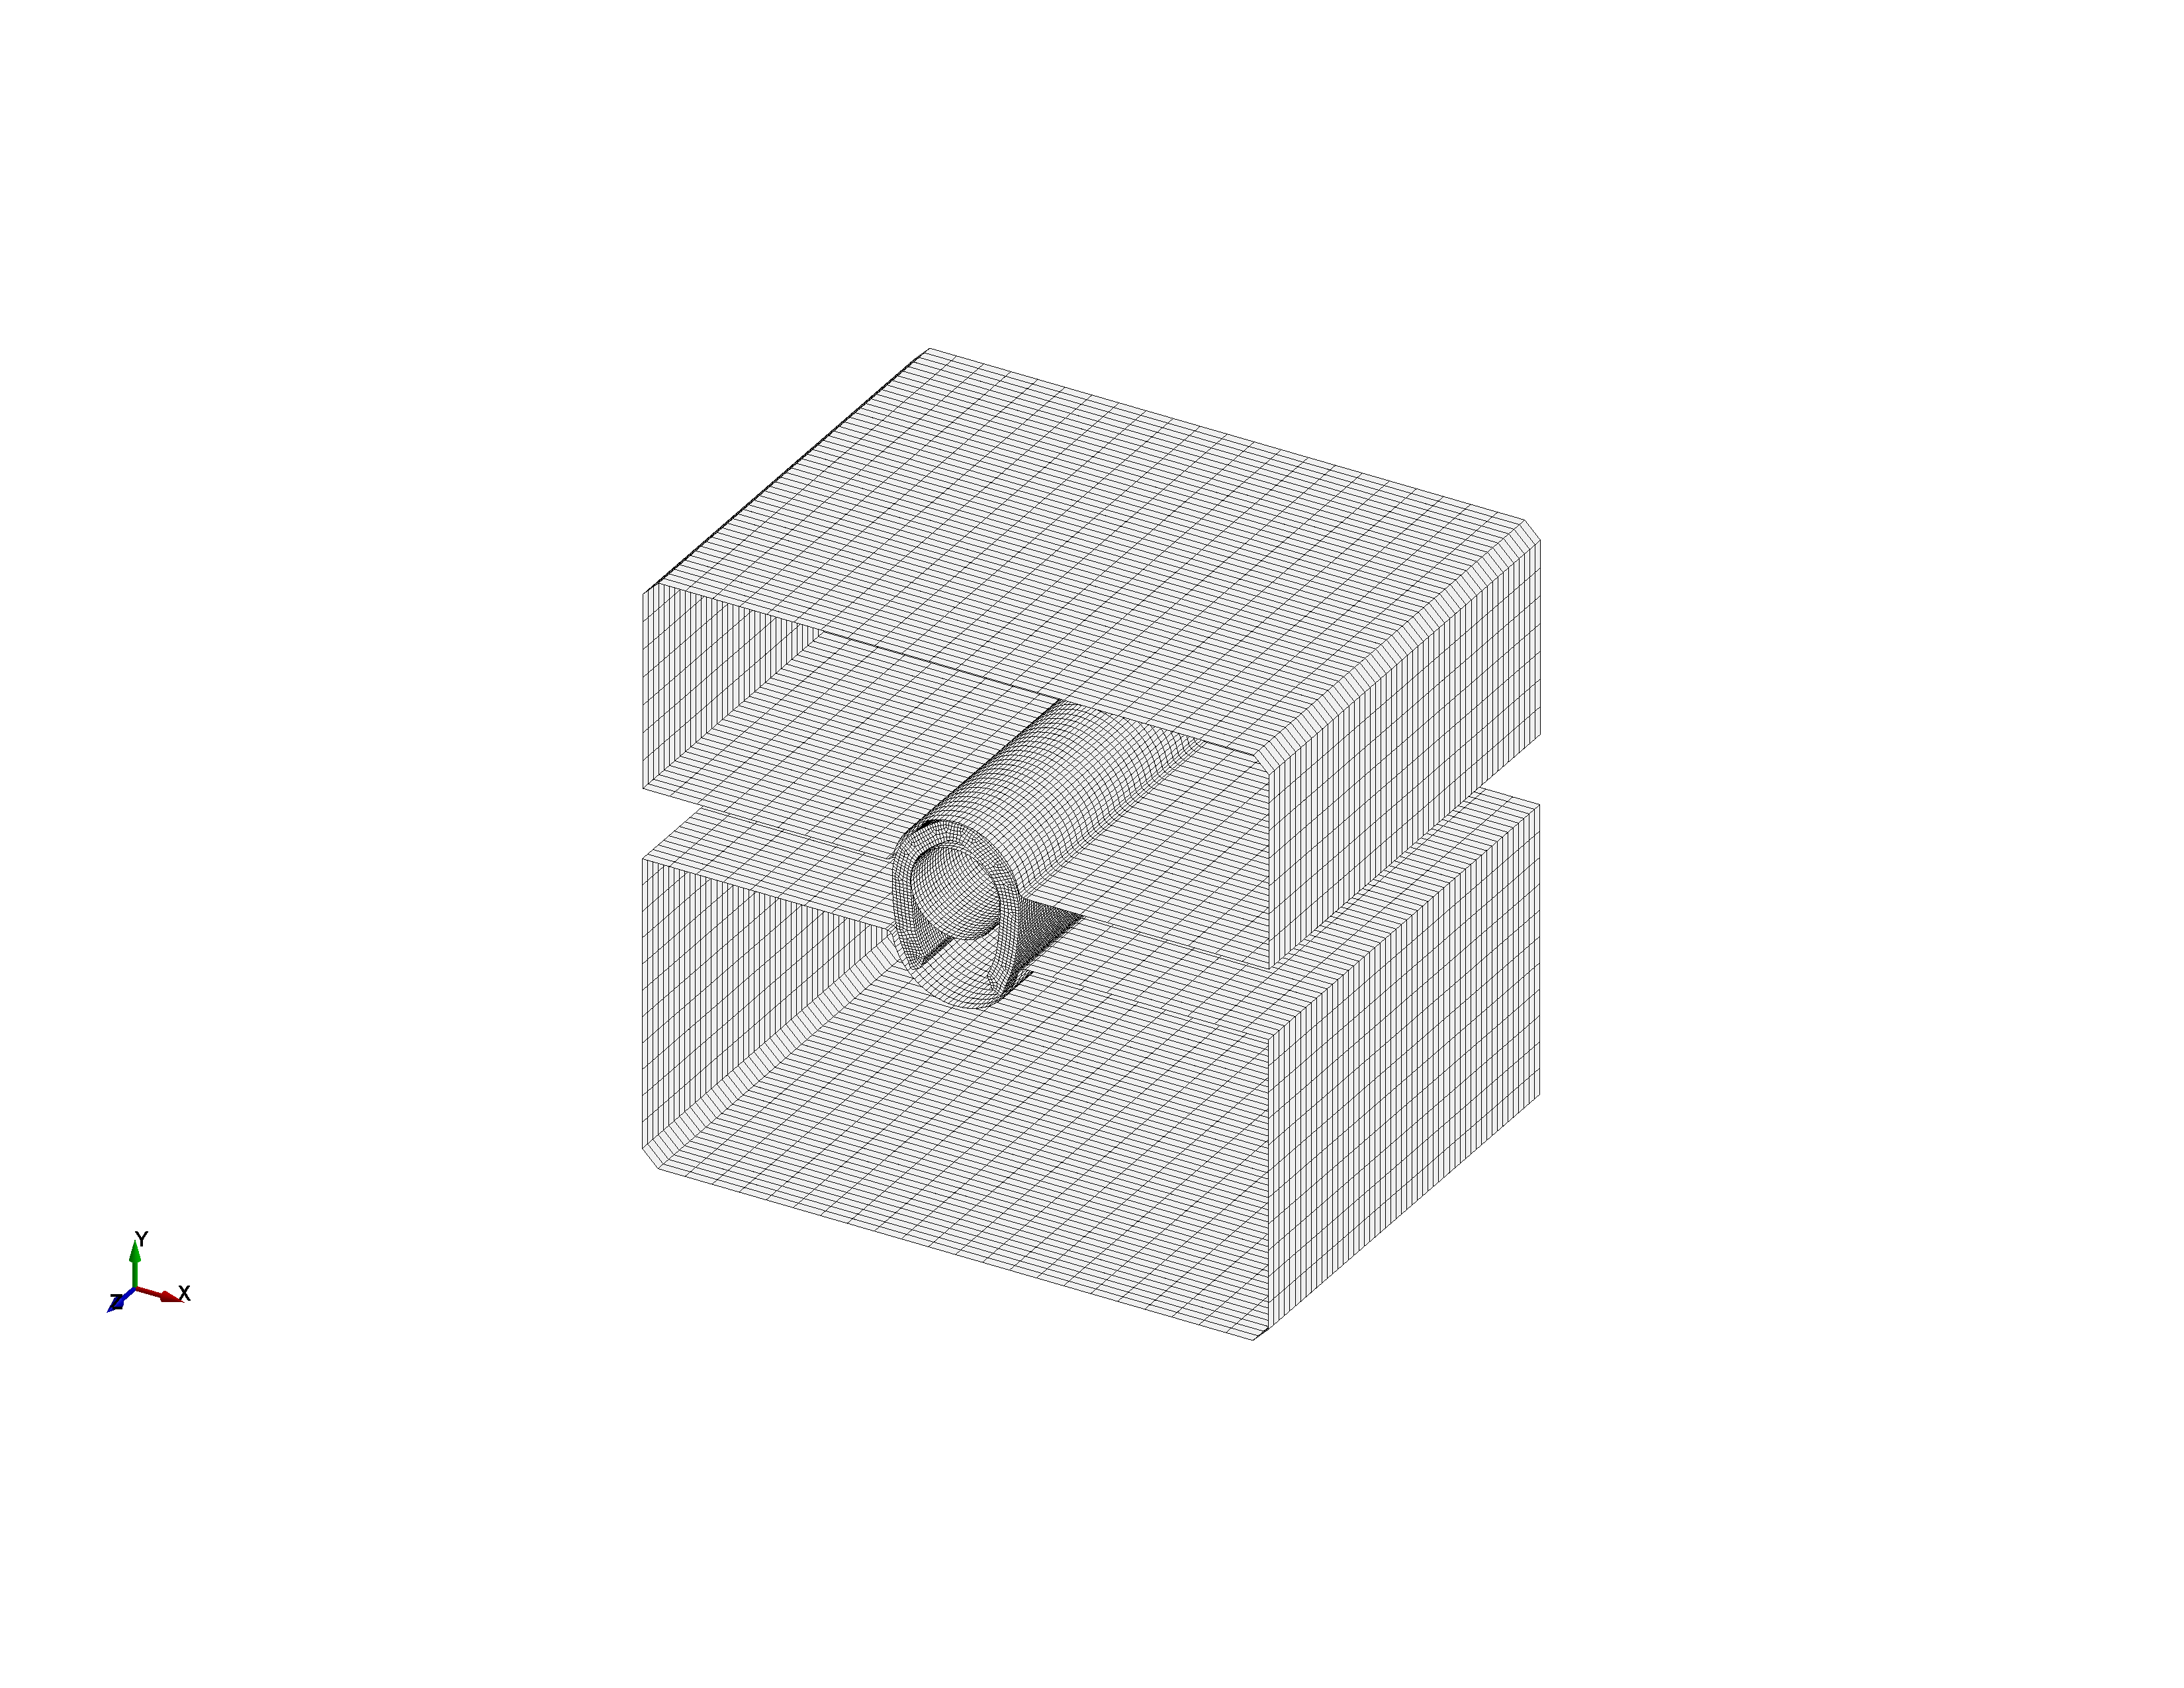
\includegraphics[width=0.6\textwidth]{src/ch3/parts_02.png}
\caption{Mallado del segundo ensamble}
\label{fig:parts_02}
\end{figure}

\begin{figure}[!h]
\centering
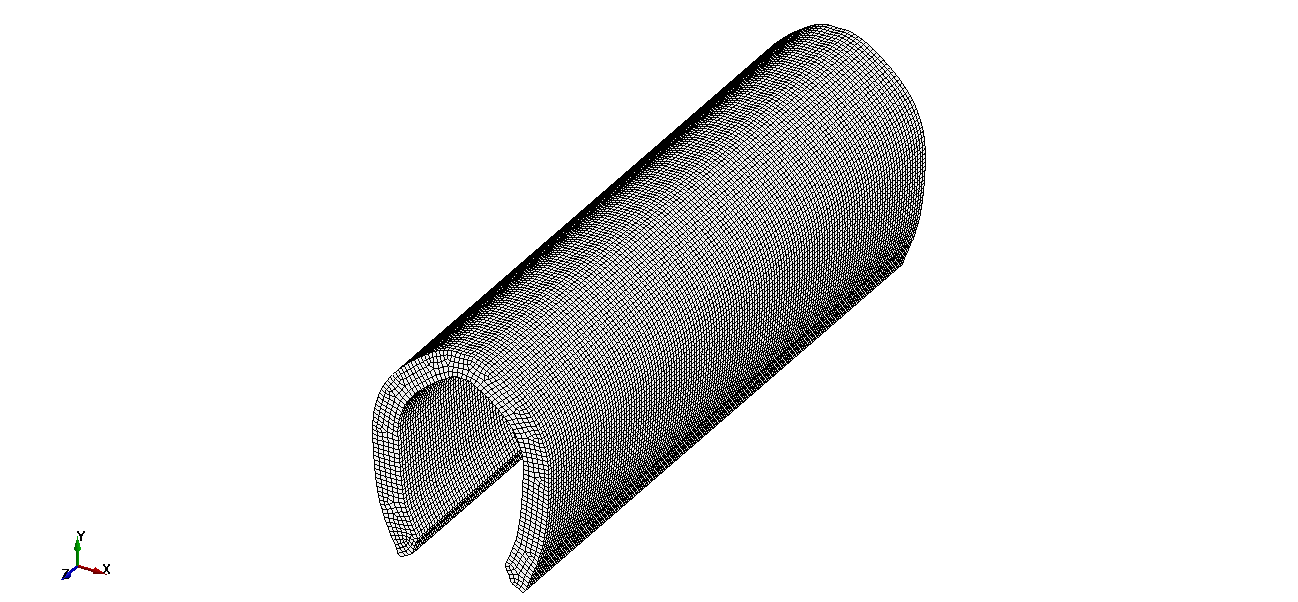
\includegraphics[width=0.5\textwidth]{src/ch3/mesh_blank_02.png}
\caption{Geometría deformada del blank importada del primer paso}
\label{fig:mesh_blank_02}
\end{figure}

\begin{figure}[!h]
\centering
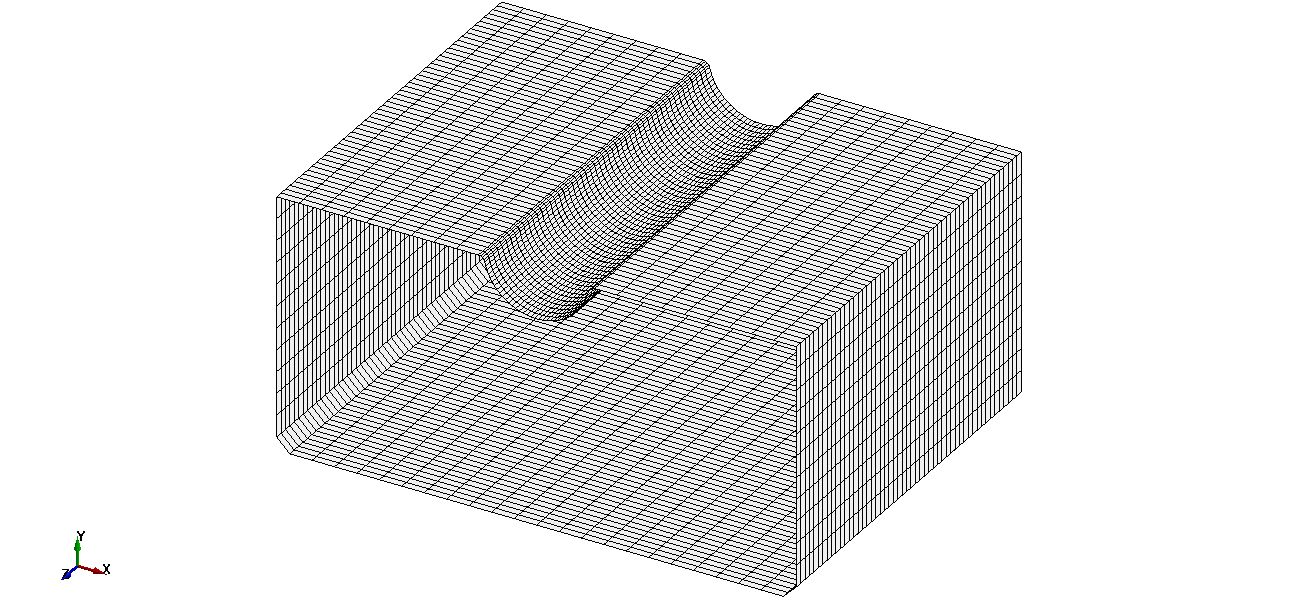
\includegraphics[width=0.5\textwidth]{src/ch3/mesh_ffi.png}
\caption{Mallado del formador final inferior}
\label{fig:mesh_ffi}
\end{figure}

\begin{figure}[!h]
\centering
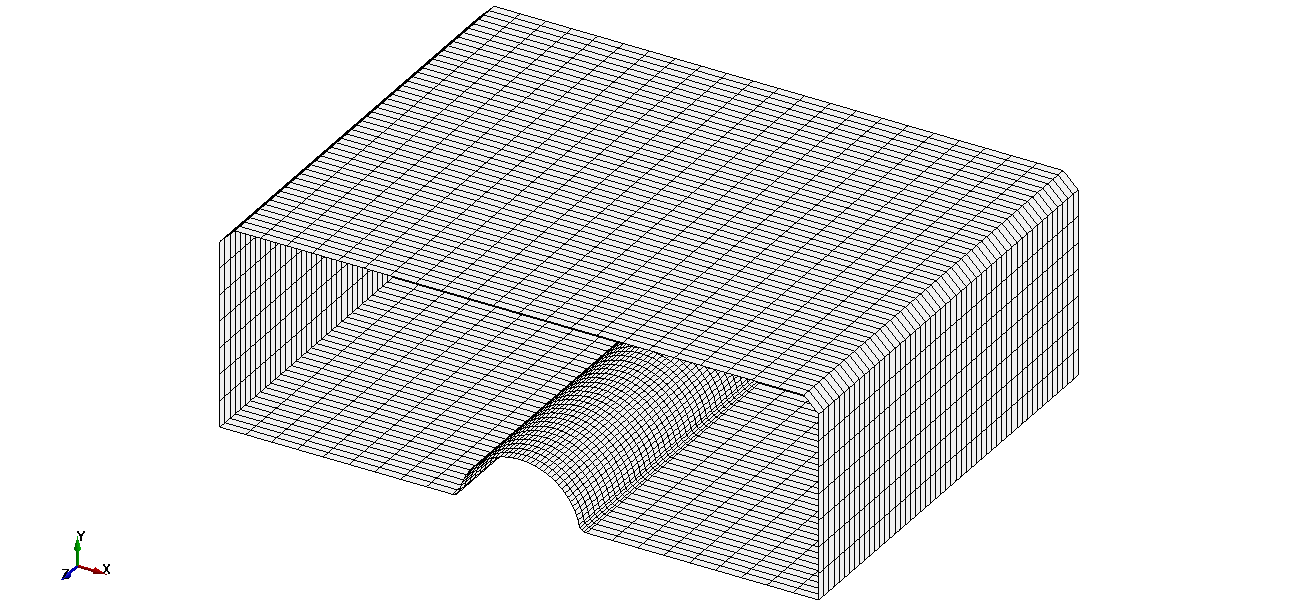
\includegraphics[width=0.5\textwidth]{src/ch3/mesh_ffs.png}
\caption{Mallado del formador final superior}
\label{fig:mesh_ffs}
\end{figure}

\begin{figure}[!h]
\centering
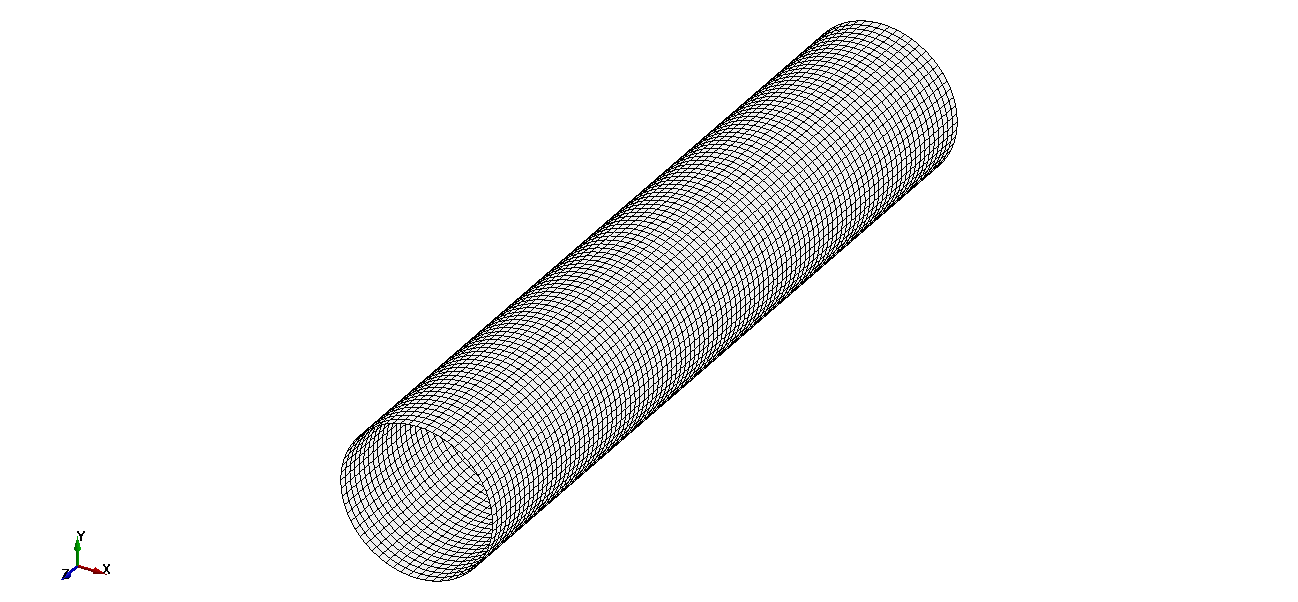
\includegraphics[width=0.5\textwidth]{src/ch3/mesh_perno.png}
\caption{Mallaod del perno formador}
\label{fig:mesh_perno}
\end{figure}


% Condiciones de frontera ==================================================================
\subsection{Condiciones de frontera}

Para efectos de la simulación el blank fue sujetado en el punto medio de cada extremo, 
en las direcciones \textit{X} y \textit{Z}, para evitar que se desplace de manera no 
deseada y con esto ayudar en la convergencia de la solución. La localización de las 
condiciones de sujeción en la parte central se debe a que se considera que la placa 
no sufre una deformación significativa en esa parte y por tanto no influirá en el campo 
de deformaciones resultante. \\

Los componentes del troquel, al ser cuerpos rígidos, la mayoría de sus 
restricciones fueron consideradas en la definición del material. En el caso de los 
formadores superiores, sólo se especificaron los desplazamientos en la dirección 
vertical Y, se utilizaron arreglos unidimensionales para especificar la relación
tiempo-desplazamiento, en todos los casos se especificó como desplazamiento de
cuerpo rígido en la dirección Y (\texttt{RBUY}), aplicándose esta condición a cada uno de los
componentes.\\

La relación tiempo-desplazamiento se definió utilizando una función de tipo
\textit{smooth-step}, cuya forma general es $f(t) = A(Bt^2 - Ct^3)$ , donde
$A$, $B$ y $C$ son constantes a ajustar para el requerimiento de desplazamiento total,
se caracteriza por tener un crecimiento lento al principio y final del intervalo
especificado, implicando una velocidad reducida de los formadores al principio y final 
del recorrido, con la finalidad de que esto facilite la estabilización y convergencia
del análisis.\\

En la figura \ref{fig:smooth_displacement_01} se muestra la gráfica del tiempo-desplazamiento 
utilizado en el primer paso del troquel. Para el segundo caso se utilizó una curva 
similar, con algunas variaciones en las constantes para disminuir la amplitud o valor máximo.\\


\begin{apdl}
*DIM,tiempo,ARRAY,400
*DIM,desplazamiento,ARRAY,400

*DO,ii,1,400
    tiempo(ii)=ii/2E3
*ENDDO

_k1 = 3.8E-7
_k2 = 1.15E-4
_k3 = -1.22

*DO,jj,1,200
    desplazamiento(jj)= _k3*(_k2*jj**2 - _k1*jj**3) - (_k3*(_k2 - _k1))
*ENDDO

*DO,kk,1,200
    desplazamiento(200+kk) = (-1)*_k3*(_k2*kk**2 - _k1*kk**3) + (_k3*(_k2*200**2 - _k1*200**3))
*ENDDO

*vplot,tiempo,desplazamiento
\end{apdl}


\begin{figure}[!h]
\centering
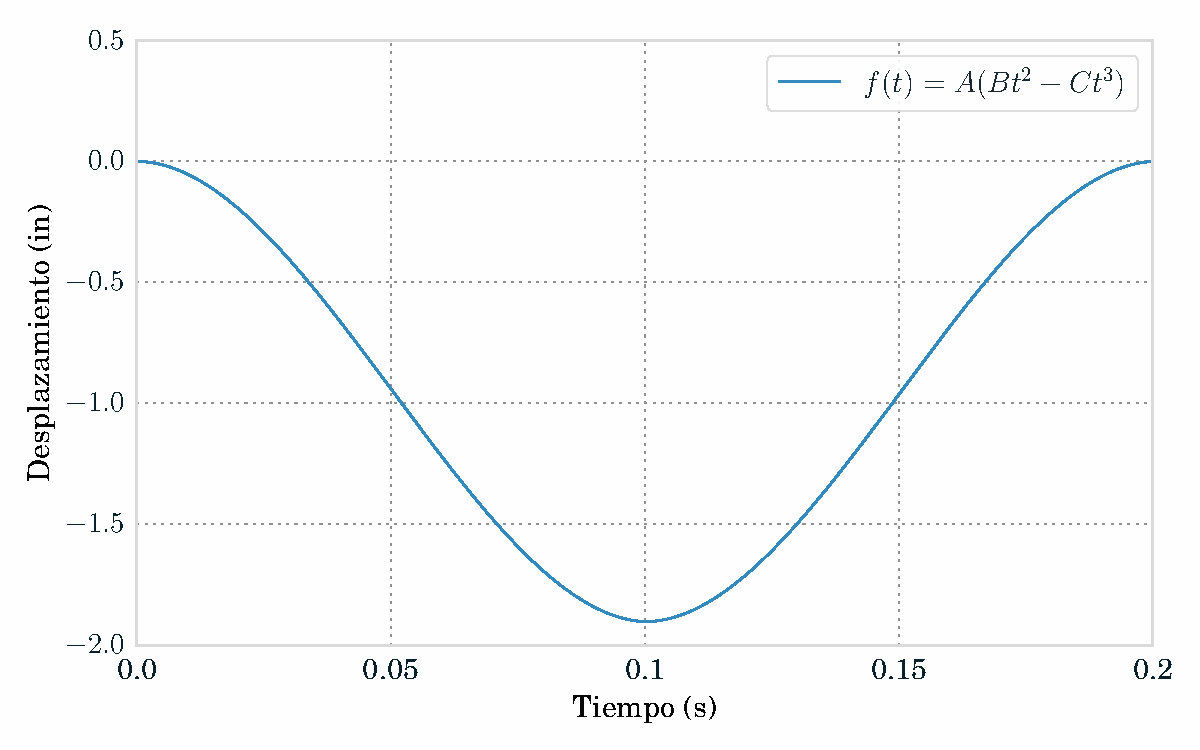
\includegraphics[scale=0.6]{src/ch3/smooth_displacement_01.pdf}
\captionof{figure}{Vector de tiempo desplazamiento}
\label{fig:smooth_displacement_01}
\end{figure}



% ==================================== CONTACTOS ============================================
\subsection{Contactos}

En la definición de contactos se utilizó un tipo de contacto superficie a superficie
general (\texttt{STS}). El programa de simulación utiliza los coeficientes de fricción 
estático ($FS$) y dinámico ($FD$) para la formulación del coeficiente friccional ($\mu_c$),
que viene dado por la ecuación :

\begin{equation}
\mu_c = FD + (FS - FD) e^{-DCv_{rel}}
\label{eq:frictional_coeff}
\end{equation}

Donde $DC$ es el coeficiente de decaimiento exponencial y $v_{rel}$ la velocidad relativa
entre las superficies en contacto ~\cite{lsdyna-manual}. Los valores del coeficiente de 
fricción estáticoy dinámico se establecieron en 0.2 y 0.1, respectivamente. ~\cite{carvill1993} \\

En la simulación del segundo paso se utilizó el contacto de tipo Single Surface (SS) para 
tomar en cuenta el contacto del blank con él mismo (cerrado del tubo) ~\cite{lsdyna-manual}, 
utilizandotambién los parámetros de fricción indicados anteriormente.


\section{Análisis experimental}


\section{Comparación de análisis numérico vs experimental}



\chapter{Análisis de resultados}

En este capítulo se presenta el análisis y discusión de los principales resultados 
obtenidos en el desarrollo de este proyecto. Del análisis por elementos finitos 
se presentan los resultados del caso bidimensional y del modelo tridimensional, comparando 
ambos casos, con la finalidad de discutir la viabilidad de utilizar un análisis de tipo 
deformación plana en una simulación de formado como esta. Además los resultados del 
análisis numérico se comparan con lo obtenido mediante el análisis experimental.\\

Además, con la finalidad de determinar algunas condiciones o parámetros que faciliten 
el análisis de procesos de formado de este tipo, se presenta una sección destinada 
a evaluar la influencia del escalamiento de masa selectivo cuya utilidad va en 
dirección de disminuir el tiempo de cómputo requerido. Asimismo se expone una sección 
referente al uso de algunos modelos de material como el bilineal isotrópico y cinemático, 
la plasticidad cinemática y curvas multilineales, para determinar si las variaciones 
en el comportamiento del material son significativas.

\section{Del análisis de elementos finitos}

\subsection{Análisis 2D}

\subsubsection{Estatus global}

Normalmente en un análisis de tipo dinámico explícito, el balance de energía juega 
un papel importante e incluso puede utilizarse como criterio de \textit{terminación}. 
Para considerar que un análisis es aceptable, la energía cinética debe representar 
menos de un 5 \% de la energía interna del modelo, de lo contrario, los efectos 
inerciales inducidos podrían afectar de manera considerable tanto la geometría 
resultante como los datos de salida. En la figura \ref{fig:energy_status_01} se observa 
que la energía cinética representa un porcentaje menor al 1\% de la energía interna, lo 
cual implica que el análisis está dentro del rango aceptable. \\

\begin{center}
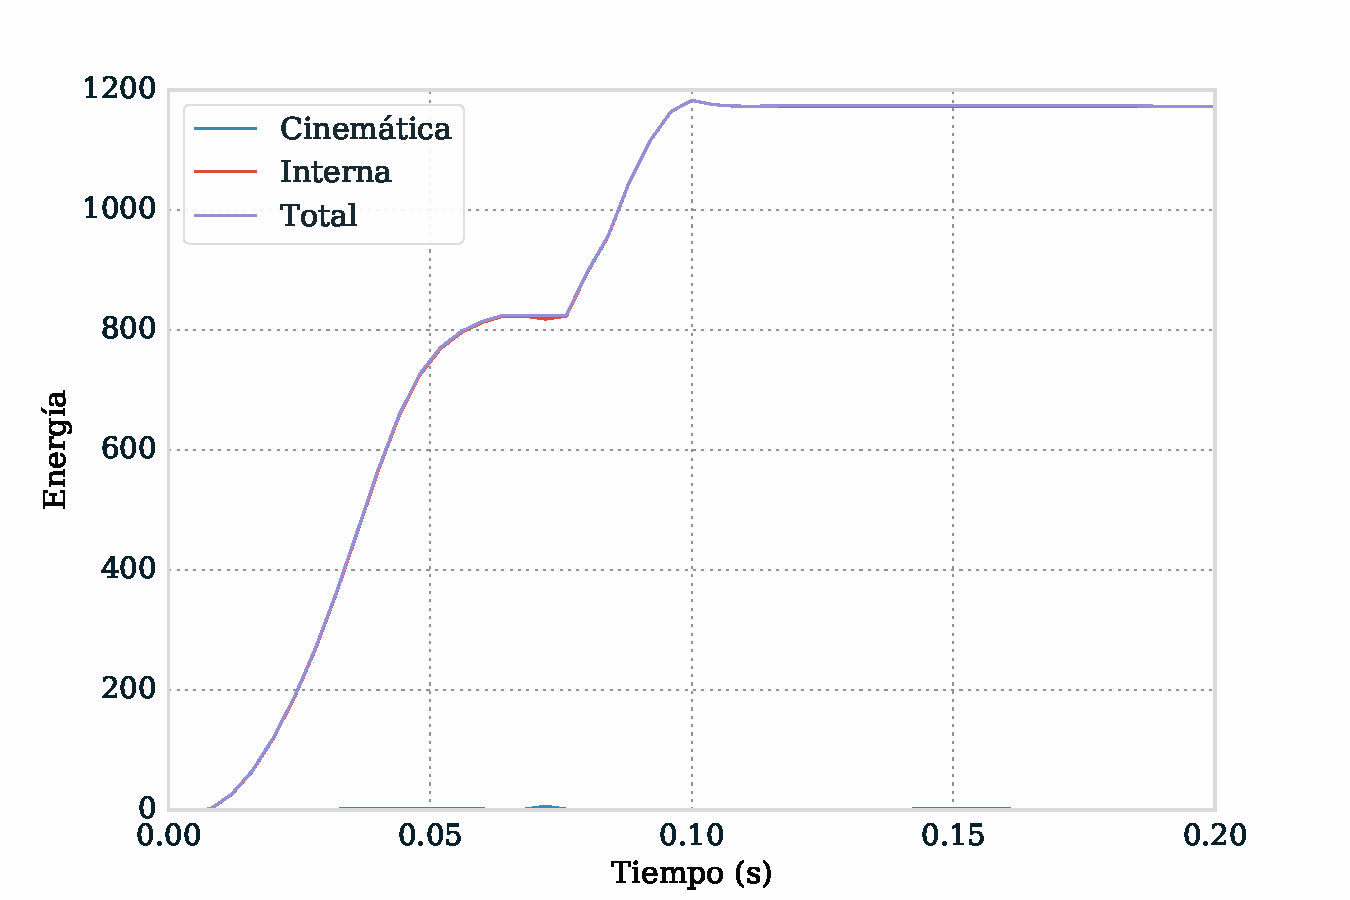
\includegraphics[width=0.8\textwidth]{src/ch4/energy_status_01.pdf}
\captionof{figure}{Variación de la energía total, interna y cinemática, primer paso}
\label{fig:energy_status_01}
\end{center}

El elemento \texttt{PLANE162}, utilizado en el mallado para el análisis bidimensional, 
tiene sólo un punto de integración, lo cual le hace robusto para grandes deformaciones 
y permite un ahorro significativo de tiempo computacional, pero esto mismo les hace 
propensos a presentar modos de energía cero. Estos modos, comúnmente referidos como 
modos de Hourglass, son de naturaleza oscilatoria y tienen periodos mucho más pequeños 
que la respuesta estructural de un sistema, resultando en estados matemáticos que físicamente 
no son posibles y que normalmente tienden a deformar la malla en forma de zigzag.
Para verificar que la deformación de Hourglass no ha influido de manera considerable 
en un análisis se debe comparar la energía interna del modelo con la energía de Hourglass, 
esta última no debe ser mayor al 10\% de la primera para considerar aceptable los 
resultados de la simulación ~\cite{lsdyna-ansys-manual}. En la gráfica de la figura \ref{fig:hourglass_internal_01} 
se muestra la energía interna vs la energía de Hourglass y se aprecia que la proporción 
varía en un rango del 1.5 a 2\%, lo cual indica que la deformación de Hourglass se encuentra 
dentro de los límites aceptables.

\begin{center}
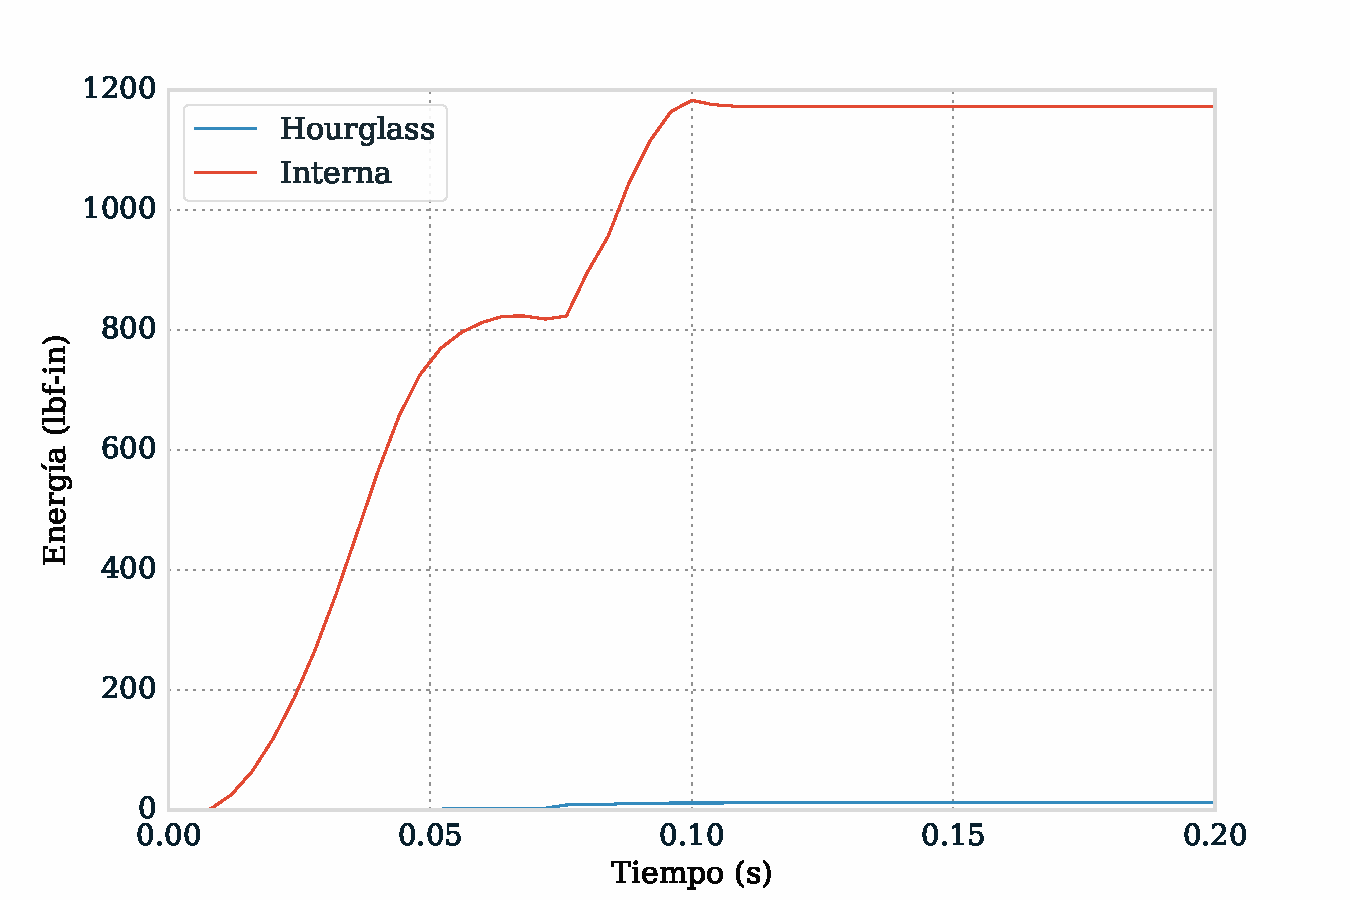
\includegraphics[width=0.8\textwidth]{src/ch4/hourglass_internal_01.pdf}
\captionof{figure}{Comparación energía interna vs energía de Hourglass}
\label{fig:hourglass_internal_01}
\end{center}


\subsubsection{Geometría resultante}

% En la figura \ref{fig:shape_sequence_01} se muestra la secuencia de formado 
% de la geometría resultante, se puede apreciar el doblado en U y el doblado 
% llevado a cabo por las levas.

% \begin{center}
% 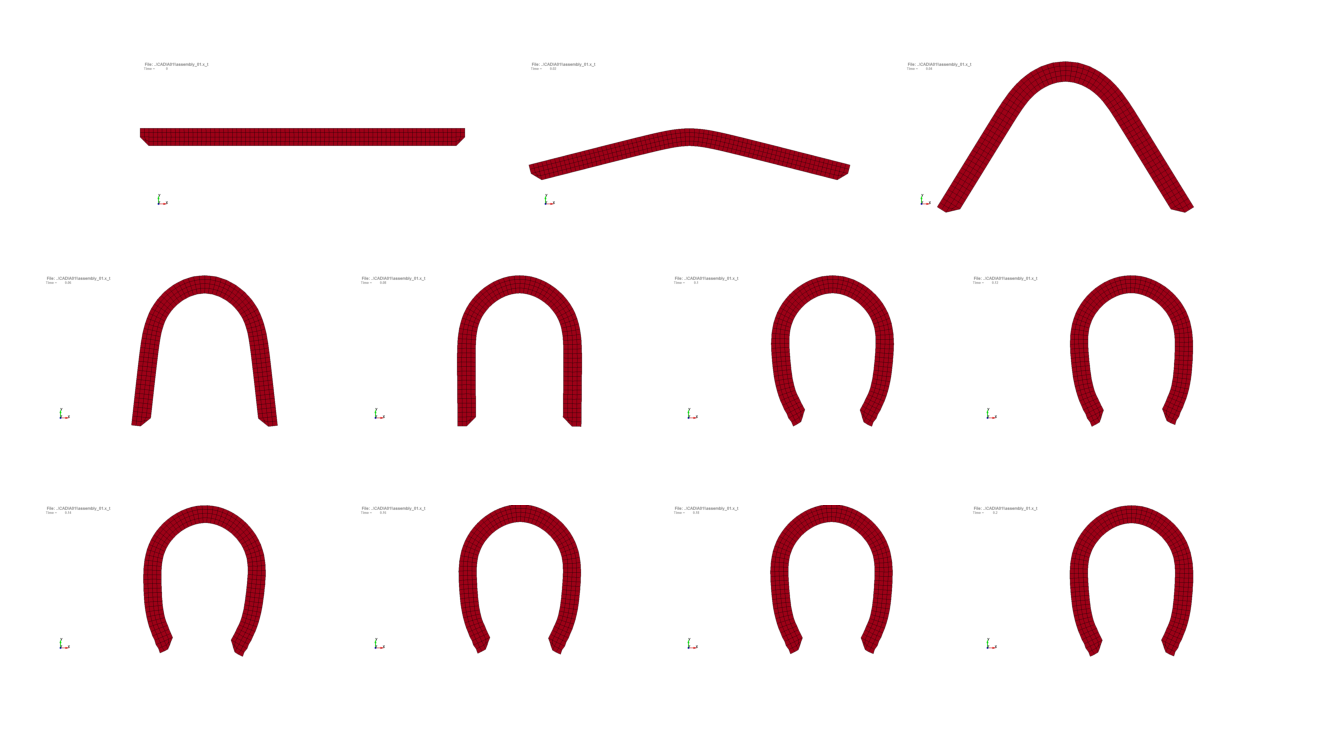
\includegraphics[width=0.95\textwidth]{src/ch4/shape_sequence_01.pdf}
% \captionof{figure}{Secuencia de la geometría resultante}
% \label{fig:shape_sequence_01}
% \end{center}

Las figuras \ref{fig:geometry_01} y \ref{fig:geometry_02} muestran las geometrías 
resultantes al final del primer y segundo paso del proceso de formado. Las formas 
obtenidas corresponden a lo esperado cuando se diseñó el herramental, y no se observan 
algún tipo de anormalidad en las formas obtenidas.

\begin{center}
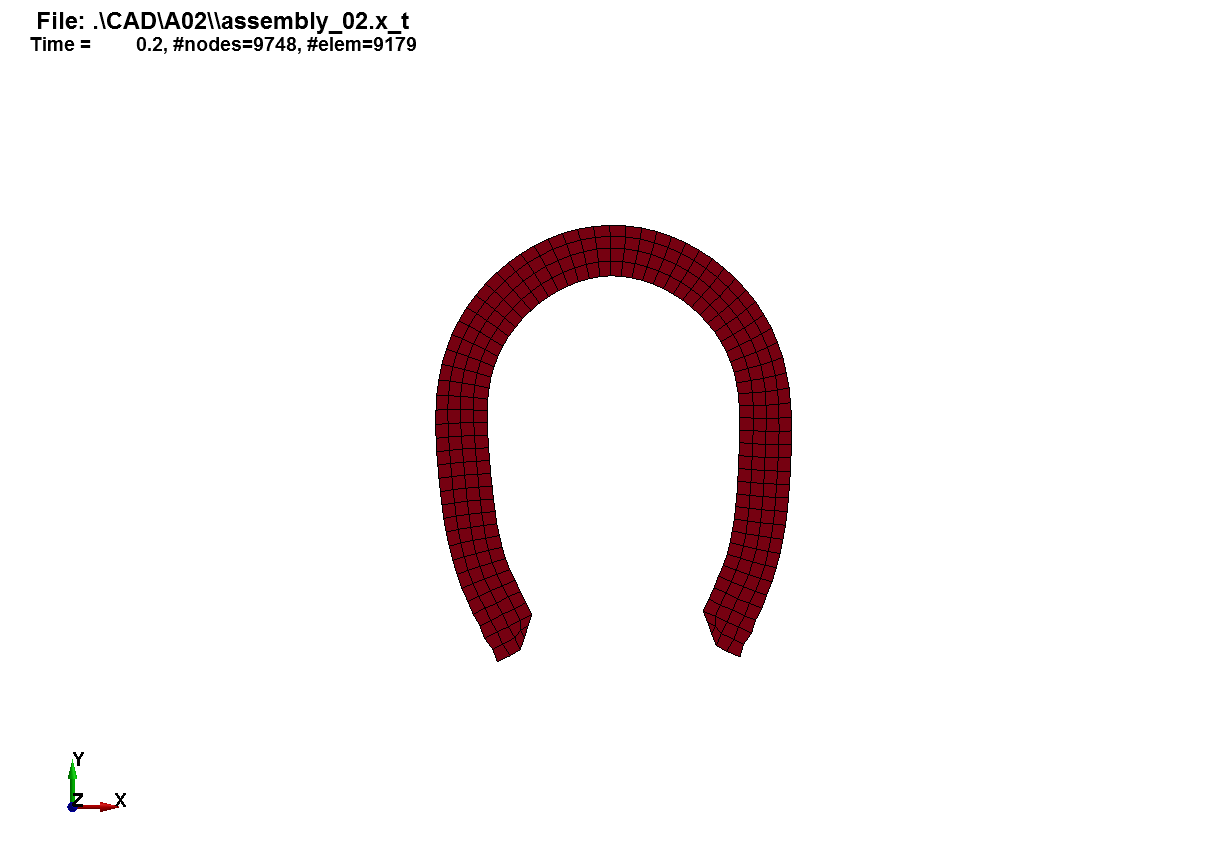
\includegraphics[width=0.75\textwidth]{src/ch4/geometry_01.png}
\captionof{figure}{Geometría resultante, primer paso}
\label{fig:geometry_01}
\end{center}

\begin{center}
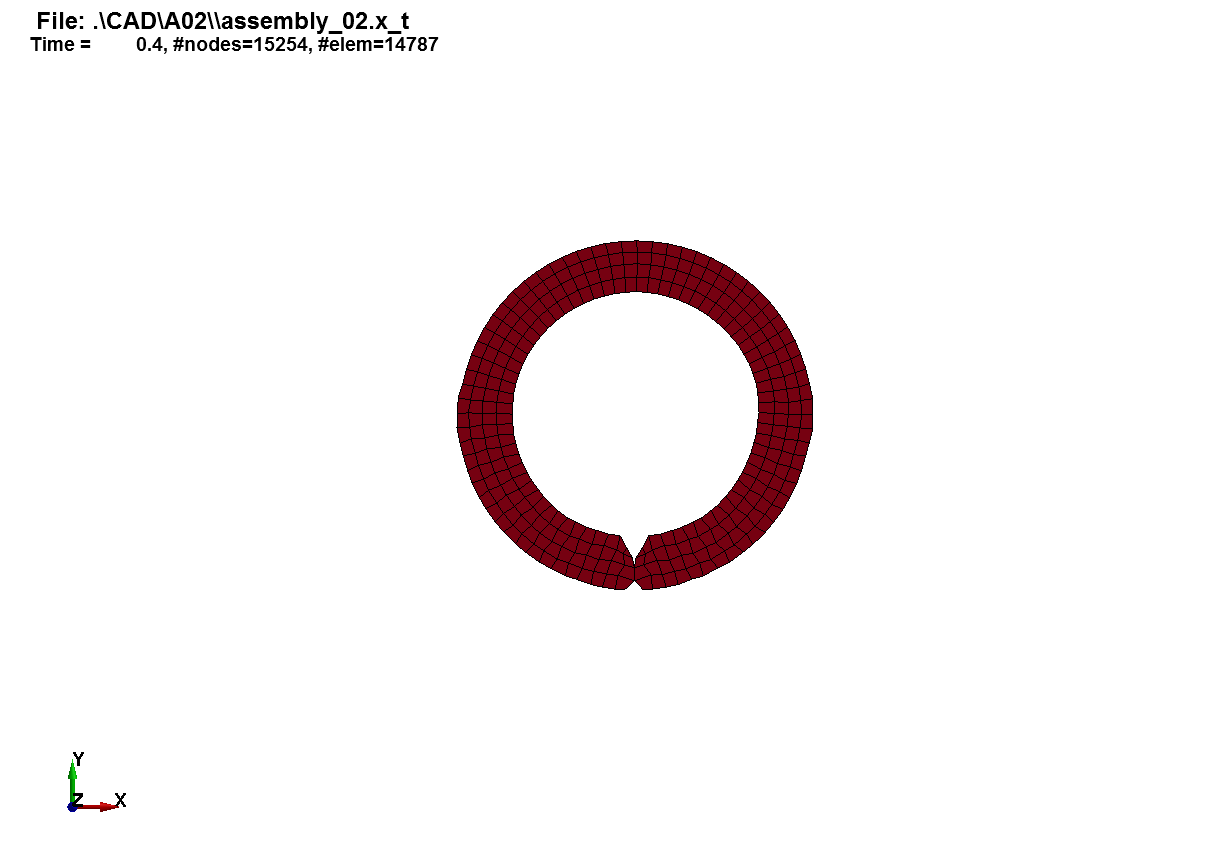
\includegraphics[width=0.75\textwidth]{src/ch4/geometry_02.png}
\captionof{figure}{Geometría resultante, segundo paso}
\label{fig:geometry_02}
\end{center}

La figura \ref{fig:thickness_variation} muestra una gráfica con las variaciones de espesor en la geometría 
final obtenida, las líneas punteadas corresponden a las tolerancias mínima y máxima del espesor. Para 
efectuar tal medición se tomaron como referencia nodos interiores y exteriores en la geometría final, 
posicionados sobre la misma vertical en la geometría inicial, y enseguida, basándose en las coordenadas 
iniciales y los desplazamientos, se obtuvo la distancia.

\begin{center}
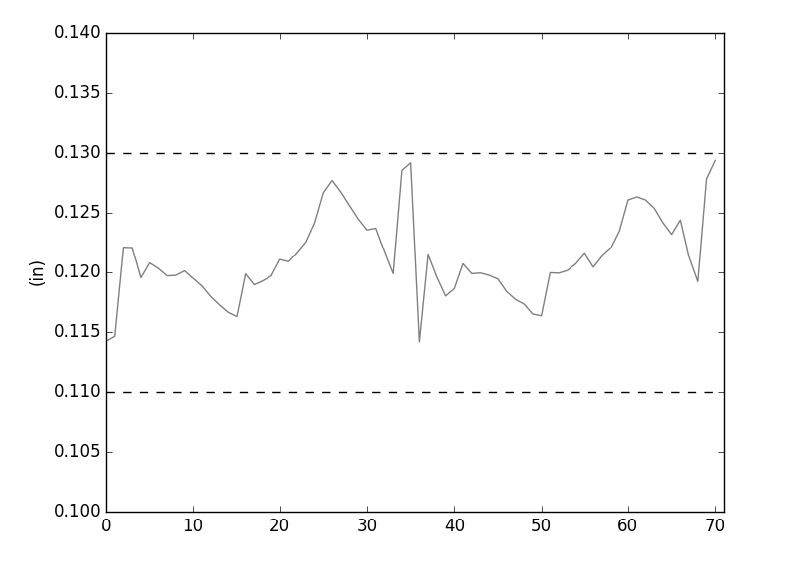
\includegraphics[width=0.75\textwidth]{src/ch4/thickness_variation.png}
\captionof{figure}{Variación del espesor de la geometría resultante}
\label{fig:thickness_variation}
\end{center}

\subsubsection{Esfuerzos}

La distribucíón de esfuerzos y sobre todo el historial del máximo se utilizó como 
un criterio comparativo  que aporta información acerca del estatus del material, 
es decir, para verificar que el material se encuentra en el rango de deformación 
plástica acorde a lo obtenido de forma experimental en la curva esfuerzo-deformación.\\

En las figuras \ref{fig:von_mises_01} y \ref{fig:von_mises_02} se muestran la 
distribución del esfuerzo de von Mises al final de la primer y segunda etapa 
del formado, respectivamente. 

\begin{center}
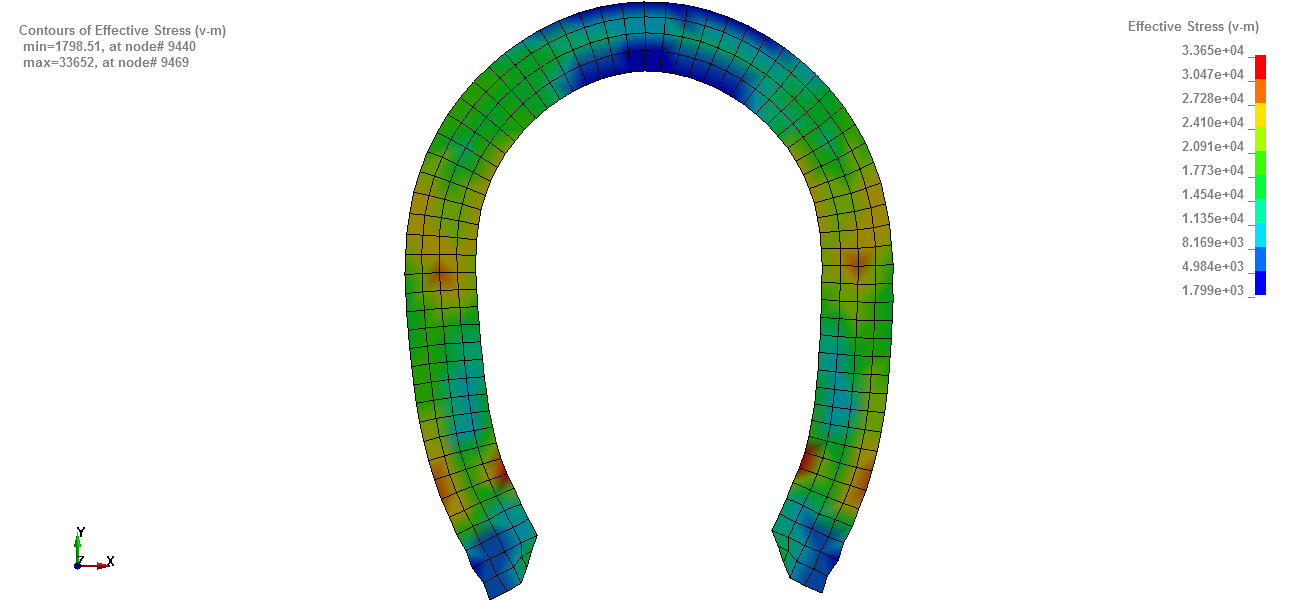
\includegraphics[width=0.75\textwidth]{src/ch4/von_mises_01.png}
\captionof{figure}{Distribución de esfuerzos de von Mises, final del primer paso}
\label{fig:von_mises_01}
\end{center}

La figura \ref{fig:von_mises_stress_01} muestra la variación del esfuerzo máximo 
de von Mises, cuyo máximo valor es de alrededor de 87,000 psi.

\begin{center}
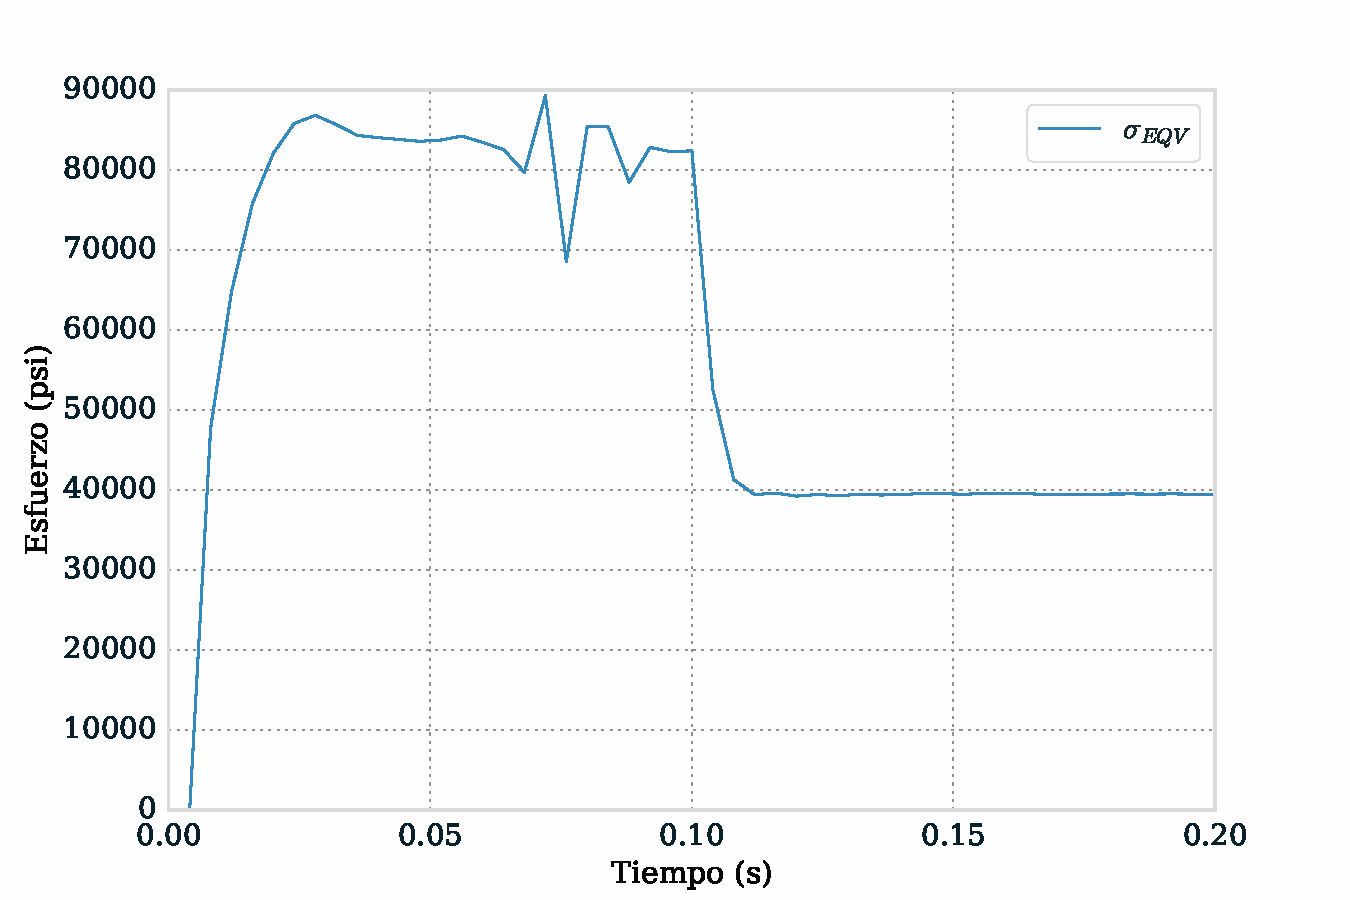
\includegraphics[width=0.75\textwidth]{src/ch4/von_mises_stress_01.pdf}
\captionof{figure}{Variación del esfuerzo máximo de von Mises}
\label{fig:von_mises_stress_01}
\end{center}

En \ref{fig:xyz_stress_01} se muestra el historial de esfuerzos en las direcciones 
X, Y, Z. Es evidente que el esfuerzo en dirección $Z$ es en general el menor de 
los tres, dado que este es calculado a partir de la ecuación de deformación plana 
que lo considera alrededor de una tercera parte de la suma de $\sigma_x$ y $\sigma_y$ para 
el caso de un acero. \\

\begin{center}
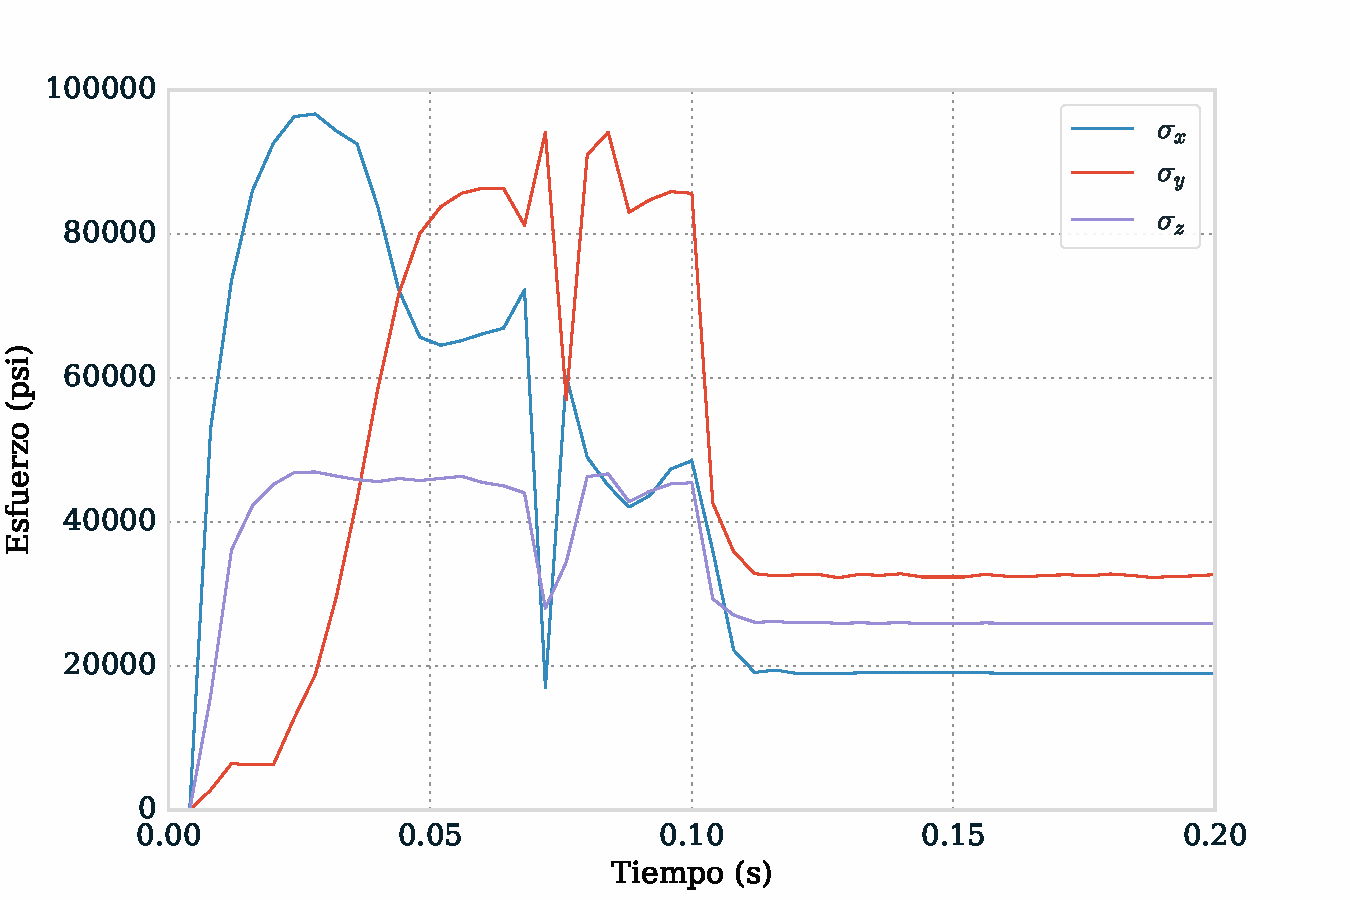
\includegraphics[width=0.75\textwidth]{src/ch4/xyz_stress_01.pdf}
\captionof{figure}{Variación de los esfuerzos máximos en dirección X,Y,Z}
\label{fig:xyz_stress_01}
\end{center}

\begin{center}
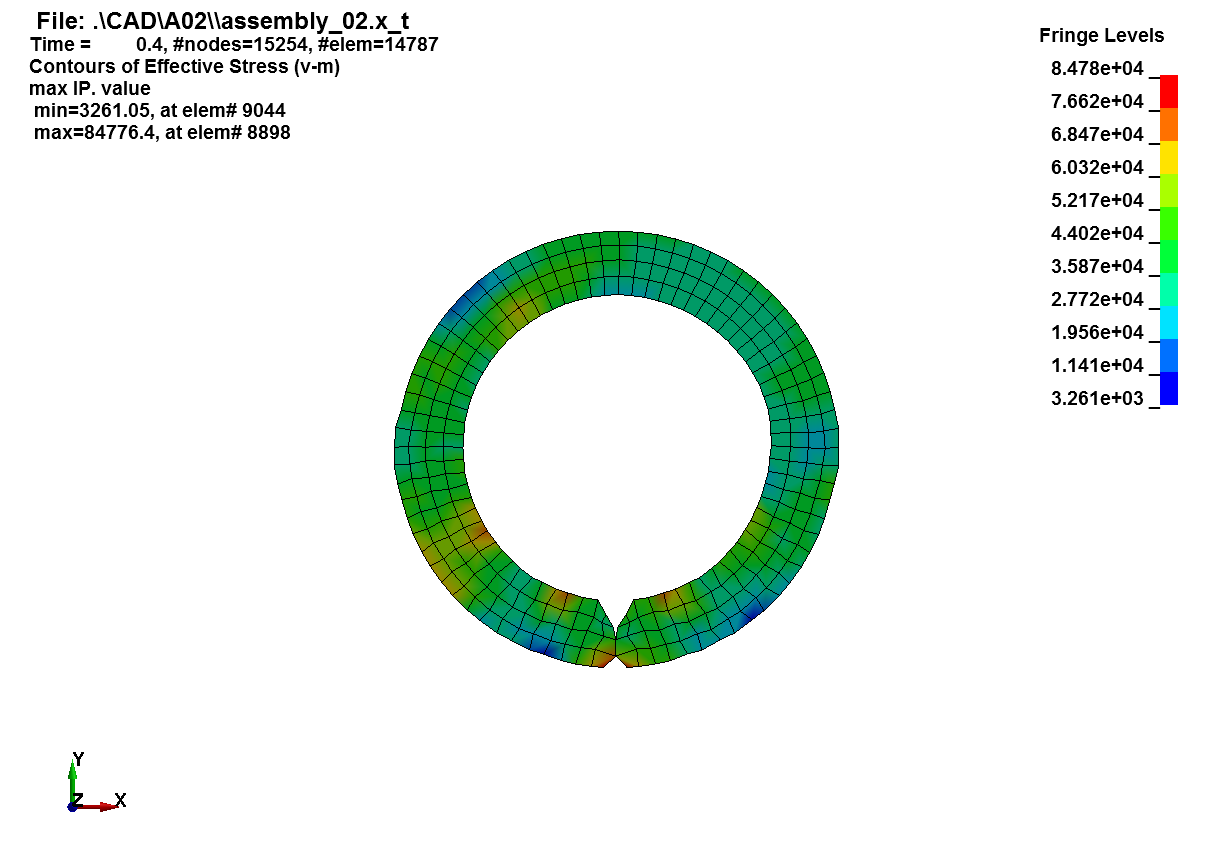
\includegraphics[width=0.75\textwidth]{src/ch4/von_mises_02.png}
\captionof{figure}{Distribución de esfuerzos de von Mises, final del segundo paso}
\label{fig:von_mises_02}
\end{center}


\subsubsection{Deformaciones}

En las figuras \ref{fig:efective_plastic_strain_01} y \ref{fig:efective_plastic_strain_02} se muestran 
las distribuciones de la deformación plástica efectiva, al final de ambas etapas del formado. 

\begin{center}
\includegraphics[width=0.75\textwidth]{src/ch4/efective_plastic_strain_01.png}
\captionof{figure}{Deformación plástica efectiva, final del primer paso}
\label{fig:efective_plastic_strain_01}
\end{center}

Tanto en \ref{fig:efective_plastic_strain_01} como en \ref{fig:efective_plastic_strain_02} se puede observar 
de manera clara una región intermedia que permanece con deformaciones muy pequeñas (región azul) o casi nulas, 
lo cual corresponde al eje neutro cuando se realiza una operación de doblado. Para una operación de doblado 
en donde el radio interior de doblado (0.285 in en este caso) es mayor al doble del espesor (0.12 in) se 
considera que el eje neutro se ubica alrededor de $0.42t$.

\begin{center}
\includegraphics[width=0.75\textwidth]{src/ch4/efective_plastic_strain_02.png}
\captionof{figure}{Deformación plástica efectiva, final del segundo paso}
\label{fig:efective_plastic_strain_02}
\end{center}

% \begin{center}
% \includegraphics[width=0.75\textwidth]{src/ch4/strain_x_02.png}
% \captionof{figure}{Deformación en dirección X, final del segundo paso}
% \label{fig:efective_plastic_strain}
% \end{center}

% \begin{center}
% \includegraphics[width=0.75\textwidth]{src/ch4/strain_y_02.png}
% \captionof{figure}{Deformación en dirección Y, final del segundo paso}
% \label{fig:efective_plastic_strain}
% \end{center}


\subsubsection{Fuerza de formado}

En la figura \ref{fig:nodal_force_01} se puede observar que la fuerza máxima de formado 
requerida para completar el primer paso es de 2500 lbf, de donde se debe considerar 
que el análisis de deformación plana se realiza en base a una pieza de trabajo de 
ancho unitario. Este resultado se puede extrapolar a la pieza real si multiplicamos el 
resultado por un factor de 3 que es lo correspondiente a la longitud del \textit{blank}, 
por tanto la fuerza requerida correspondería a 7500 lbf.\\

De la gráfica de \ref{fig:nodal_force_01} se puede observar también que existen dos máximos 
locales correspondientes a la fuerza requerida para la operación de los formadores superiores y 
de las levas formadoras, de manera respectiva.\\

El primer máximo local, que corresponde al doblado realizado por los formadores, se puede 
comparar con la fuerza calculada de manera analítica a partir de la ecuación \ref{eq:fuerza_doblado}, 
de la cual se tiene:

\begin{equation}\label{eq:fuerza_doblado}
F = \frac{K S_{t} w t^2}{D} = \frac{(1.33)(52000)(3)(0.12)^2}{0.93} = 3212 \text{lbf}
\end{equation}

\begin{center}
\includegraphics[width=0.75\textwidth]{src/ch4/nodal_force_01.pdf}
\captionof{figure}{Fuerza de formado requerida, primer paso}
\label{fig:nodal_force_01}
\end{center}


\subsubsection{Influencia del escalamiento de masa}\label{sec:mass-scaling-results}

En la sección \ref{sec:mass-scaling} se describió el proceso para utilizar el escalamiento de masa 
selectivo en un análisis de tipo dinámico explícito, cuyo objetivo es reducir el tiempo de 
solución de una simulación mediante la introducción controlada de \textit{masa artificial} que implica 
un aumento en la densidad del material y esto a su vez la reducción de los intervalos de tiempo.\\

En lo subsiguiente se presenta el análisis de cinco simulaciones realizadas con escalamientos de 
masa selectivo, en donde el tamaño mínimo del paso de tiempo se varía desde $1x10^{-7}$ hasta 
$5x10^{-7}$.\\

La figura \ref{fig:ms_sol_time} muestra la variación del tiempo de solución (CPU Time) comparado con 
el porcentaje de masa agregado. Se observa que la curva resultante muestra el comportamiento de 
una función exponencial decreciente y que con un 12\% de masa adicional se puede reducir el tiempo 
de solución hasta un 30\% respecto al tiempo de solución sin escalamiento de masa.

\begin{center}
\includegraphics[width=0.75\textwidth]{src/ch4/ms_sol_time.pdf}
\captionof{figure}{Tiempo de solución para diversos escalamientos de masa}
\label{fig:ms_sol_time}
\end{center}

En \ref{fig:ms_von_mises} se muestra la variación del esfuerzo equivalente máximo de von Mises, cuando 
se aplica el escalamiento de masa. Se puede observar que la variación entre cada uno de los casos 
es mínima en todo el hsitorial de tiempo, habiendo una diferencia significativa en el tiempo 
correspondiente a cuando los formadores superiores dejan de actuar y las levas aún no interactúan 
con la pieza de trabajo.

\begin{center}
\includegraphics[width=0.75\textwidth]{src/ch4/ms_von_mises.pdf}
\captionof{figure}{Variación del esfuerzo de von Mises utilizando escalamiento de masa}
\label{fig:ms_von_mises}
\end{center}

En \ref{fig:ms_force} se muestra la variación de la fuerza de formado, se observa que el 
comportamiento es prácticamente similar para todos los casos.

\begin{center}
\includegraphics[width=0.75\textwidth]{src/ch4/ms_force.pdf}
\captionof{figure}{Variación de la fuerza de formado usando escalamiento de masa}
\label{fig:ms_force}
\end{center}

Con lo observado, se puede asumir que la influencia del escalamiento de masa, agregando hasta alrededor 
de un 110\% de masa, no es significativa, y permite reducir hasta en un 90\% el tiempo de solución de 
un análisis dinámico-explícito, lo cual representa una enorme ventaja.\\

\textbf{Escalamiento de masa excesivo} \\

Un escalamiento de masa excesivo normalmente conlleva a un resultado alejado de la realidad, las formas 
geométricas deformadas tienden a no corresponder con lo esperado, debido a que los efectos de la inercia 
inducida por la introducción de masa artificial son muy exagerados. Por ejemplo, en la figura 
\ref{fig:ms_excessive} se muestra una simulación que resulta de utilizar un escalamiento de masa bastante 
exagerado (un ratio mayor a 400 de \textit{masa agregada}); se puede observar claramente que la geometría 
de la pieza de trabajo se deforma hasta una configuración improbable para un material rígido como el acero, 
aún cuando los formadores superiores no están en contacto directo en ese instante, esto debido a que la 
energía cinética (que aumenta con la masa) del modelo representa una fracción superior al 10\% de la 
energía interna.\\

\begin{center}
\includegraphics[width=0.85\textwidth]{src/ch4/ms_excessive.png}
\captionof{figure}{Algunos efectos del escalamiento excesivo de masa}
\label{fig:ms_excessive}
\end{center}

\subsubsection{Modelos de material}

En las figuras  \ref{fig:mdm_von_mises} y \ref{fig:mdm_force} se muestran las gráficas correspondientes 
al esfuerzo máximo de von Mises y la fuerza de formado, respectivamente, de la evaluación de los diversos 
modelos de material que ahí se listan.\\

Tanto la variación de los esfuerzos, como la de la fuerza de formado, es poco significativa, mostrando 
un comportamiento similar en ambos casos para todos los modelos de material utilizados. La 
diferencia más notoria ocurre en los esfuerzos residuales que quedan al finalizar el proceso 
de formado, en donde se observa una diferencia de alrededor de un 20\% del modelo multilineal 
respecto al bilineal cinemático.

\begin{center}
\includegraphics[width=0.75\textwidth]{src/ch4/mdm_von_mises.pdf}
\captionof{figure}{Variación de la fuerza de formado usando escalamiento de masa}
\label{fig:mdm_von_mises}
\end{center}

\begin{center}
\includegraphics[width=0.75\textwidth]{src/ch4/mdm_force.pdf}
\captionof{figure}{Variación de la fuerza de formado usando escalamiento de masa}
\label{fig:mdm_force}
\end{center}

\subsection{Análisis 3D}


% \subsubsection{Estatus global}

% \begin{center}
% \includegraphics[width=0.75\textwidth]{src/ch4/energy_status_3d.png}
% \captionof{figure}{Energía interna, cinética y total}
% \label{fig:von_mises_3D_01}
% \end{center}

\subsubsection{Esfuerzos}


\begin{center}
\includegraphics[width=0.75\textwidth]{src/ch4/von_mises_3D_01.png}
\captionof{figure}{Distribución del esfuerzo de von Mises}
\label{fig:von_mises_3D_01}
\end{center}

\begin{center}
\includegraphics[width=0.75\textwidth]{src/ch4/von_mises_3D_02.png}
\captionof{figure}{Distribución del esfuerzo de von Mises, segundo paso}
\label{fig:von_mises_3D_02}
\end{center}

\subsubsection{Deformaciones}

\begin{center}
\includegraphics[width=0.75\textwidth]{src/ch4/eqv_strain_01.png}
\captionof{figure}{Deformación plástica equivalente, primer paso}
\label{fig:eqv_strain_01}
\end{center}


\subsection{Comparación 2D vs 3D}

En esta sección se presenta un análisis comparativo entre el análisis bidimensional 
y el análisis en tres dimensiones.

\subsubsection{Tiempo de cómputo}

\subsubsection{Fuerza de formado}


\section{Del análisis experimental}



\chapter*{CONCLUSIONES}
\addcontentsline{toc}{chapter}{CONCLUSIONES}

% \mybox{CONCLUSIONES DEL TRABAJO DE TESIS}

En este proyecto se desarrolló la simulación por elementos finitos del proceso de formado 
de un tubo de acero AISI 1018, mediante un enfoque dinámico explícito. De acuerdo a lo 
planteado inicialmente se obtuvieron resultados aceptables, en términos de las geometrías 
resultantes y las fuerzas requeridas respecto a la capacidad de trabajo de la prensas 
disponibles en producción.\\

La simulación por elementos finitos es una herramienta auxiliar muy útil en el proceso de 
diseño y validación de herramentales, y proporciona una ventaja competitiva si se utiliza 
de forma adecuada, para lo cual hace falta caracterizar de manera correcta el fenónemo 
que se está simulando, tomando en cuenta todas las cuestiones que puedan influir 
en el proceso. Del análisis por elementos finitos realizado durante este proyecto 
se pudieron extraer algunas consideraciones y/o conclusiones que resultan válidas 
para la mayoría de los procesos de doblado mediante un análisis de tipo dinámico explícito, mismas 
que se describen enseguida.\\

Es importante identificar cuándo se tienen análisis que pueden tratarse como casos simplificados 
de esfuerzo plano o deformación plana, ya que esto puede representar una reducción significativa 
de tiempo y recursos computacionales. En el caso del modelo analizado en este proyecto, asumir 
una condición de deformación plana ha generado resultados bastante similares a los obtenidos 
mediante la simulación del modelo tridimensional, con un error relativo de 4\% para la fuerza 
de formado máxima en el cerrado del tubo, y menor al 1\% en la etapa del doblado en U. 
Respecto al tiempo de cómputo requerido, se pudo observar que un análisis bidimensional 
permite reducirlo hasta en un 97\% respecto a un modelo tridimensional.
Cuando se hace un análisis de tipo deformación plana es importante tomar en cuenta que este 
se realiza considerando un especimen de espesor unitario, y por tanto hay que hacer los ajustes 
o correcciones necesarias en caso de que el modelo completo difiera de esta característica. \\

El fenómeno de la fricción en un proceso de doblado no es tan significativo, puesto que no 
es necesario realizar una lubricación adicional o especial, como puede ocurrir en casos 
de embutición profunda, de modo que en análisis por elementos finitos se puede asumir 
un coeficiente friccional ordinario de interacción metal-metal de 0.2, el cual da resultados 
aceptables. De hecho, variando el coeficiente de fricción en el análisis realizado, se observó 
muy poca diferencia en las geometrías deformadas y los resultados obtenidos en un rango de 0.05-0.3, 
con valores menores o casi nulos de fricción la pieza tiende a deslizarse sobre el formador 
inferior y en consecuencia se obtiene una geometría resultante asimétrica.\\

El escalamiento de masa selectivo en un análisis de tipo dinámico explícito representa una 
opción bastante viable para cuando se tienen recursos computacionales limitados y se 
requiere ejecutar un análisis que no admite otro tipo de simplificaciones. Esto requiere 
obviamente de un criterio de selección del tamaño de los pasos de tiempo y/o del porcentaje 
de \textit{masa artificial} que se adiciona. De acuerdo al manual teórico del software 
utilizado, es posible, en la mayoría de los casos, disminuir en un 50\% el tiempo de CPU 
empleado agregando una cantidad alrededor de 0.001\% de masa adicional.\\

Para el análisis experimental se utilizaron galgas extensométricas, cuya lectura se redujo  
al doblado en U del primer paso, debido a las limitaciones inherentes a la instrumentación y las 
grandes deformaciones presentes en el proceso de formado. Comparando los resultados obtenidos 
de forma experimental con los de la simulación del modelo bidimensional, se observó un comportamiento 
bastante similar en la curva de la relación fuerza-deformación, con una correlación del 98\% , 
lo cual implica que el modelo del material utilizado y las propiedades establecidas en el análisis 
por elementos finitos proporcionan resultados adecuados para procesos de este tipo.  \\

Con lo realizado en este proyecto, la empresa tendrá un precedente y punto de partida para la 
implementación del uso de software de análisis por elementos finitos para la simulación de 
partes estampadas, desde el tipo de análisis a realizar sabiendo a priori las consideraciones aquí 
expuestas, los parámetros de interés para la simulación, modelos constitutivos, así como 
conocer los datos de salida que pueden obtenerse de una simulación de este tipo. Puesto que la 
mayoría de las partes estampadas fabricadas en la empresa, se realizan mediante operaciones de 
doblado con láminas de similar espesor, lo aquí estudiado es aplicable y adaptable para 
la simulación de desarrollos futuros.

% ==================================================== Referencias ====================================================
\bibliographystyle{unsrt}
\bibliography{bibs}

% ==================================================== Anexos =========================================================
\chapter*{Anexos}
\addcontentsline{toc}{chapter}{Anexos}
\renewcommand{\thesection}{\Alph{section}}

\section{APDL Scripts}

\subsection{Definición de materiales}\label{sec:definicion-materiales}

\begin{apdl}
! Para el formador inferior
MP,EX,2,29E6 ! psi
MP,NUXY,2,0.3 ! 
MP,DENS,2,0.00073 ! lbf s^2 / in^4
EDMP,rigid,2,7,7

! Formador superior izquierdo
MP,EX,3,29E6 ! psi
MP,NUXY,3,0.3 ! 
MP,DENS,3,0.00073 ! lbf s^2 / in^4
EDMP,rigid,3,6,7

! Formador superior derecho
MP,EX,4,29E6 ! psi
MP,NUXY,4,0.3 ! 
MP,DENS,4,0.00073 ! lbf s^2 / in^4
EDMP,rigid,4,6,7

! Leva izquierda
MP,EX,5,29E6 ! psi
MP,NUXY,5,0.3 ! 
MP,DENS,5,0.00073 ! lbf s^2 / in^4
EDMP,rigid,5,6,4

! Leva derecha
MP,EX,6,29E6 ! psi
MP,NUXY,6,0.3 ! 
MP,DENS,6,0.00073 ! lbf s^2 / in^4
EDMP,rigid,6,6,4

! Para el blank
! Propiedades elásticas
MP,EX,1,29E6 ! psi
MP,NUXY,1,0.3 ! 
MP,DENS,1,0.00073 ! lbf s^2 / in^4

! Definir un arreglo para la deformación plástica verdadera
*dim,strn,,6
! Definir un arreglo para el esfuerzo verdadero
*dim,strs,,6

! Deformación (in/in)
strn(1) = 0.0, 0.0293, 0.0772, 0.1562, 0.2356, 0.344943

! Esfuerzo (psi)
strs(1) = 52489.4,60585.8,70710,76809.3,80244.3,82574.1

! Curva #1: Abscisa=deformación & Ordenada=esfuerzo
edcurve,add,1,strn,strs 

! Especificar Power Law #8 para el material #1
TB,PLAW,1,,,8  ! Piecewise Linear Plasticity

! Usar curva #1 para la relación esfuerzo-deformación
TBDATA,1,52e3 ! Esfuerzo de fluencia (psi)
TBDATA,3,.75 ! Deformación de falla
TBDATA,4,40.0 ! C (Parámetro de tasa de deformación)
TBDATA,5,0.1 ! P (Parámetro de tasa de deformación)
TBDATA,6,1 ! ID de la curva
\end{apdl}


\subsection{Definición de los arrays tiempo-desplazamiento}\label{sec:tiempo-desplazamiento}

\begin{apdl}
*DIM,tiempo,ARRAY,400
*DIM,desplazamiento,ARRAY,400

*DO,ii,1,400
    tiempo(ii)=ii/2E3
*ENDDO

_k1 = 3.8E-7
_k2 = 1.15E-4
_k3 = -1.22

*DO,jj,1,200
    desplazamiento(jj)= _k3*(_k2*jj**2 - _k1*jj**3) - (_k3*(_k2 - _k1))
*ENDDO

*DO,kk,1,200
    desplazamiento(200+kk) = (-1)*_k3*(_k2*kk**2 - _k1*kk**3) + (_k3*(_k2*200**2 - _k1*200**3))
*ENDDO

*vplot,tiempo,desplazamiento
\end{apdl}


\end{document}

% chrome://settings/resetProfileSettings